 \documentclass[12pt, a4paper]{report}
 \usepackage[dvipdfmx]{graphicx}
 \usepackage{listings}
 \usepackage[pdftex]{hyperref}
 \usepackage{url}
 \usepackage{graphicx,color}
 \usepackage[font=scriptsize]{caption}
 \usepackage{subcaption}
 \usepackage{fullpage}
 \usepackage{footnote}
 \usepackage{pdfpages}
 \usepackage{amsmath}
 \usepackage{longtable}
 \usepackage{tcolorbox}
\usepackage{longtable}
\usepackage[brazil]{babel}
\usepackage{listings}
\usepackage{float}


 \newcommand\tab[1][0.5cm]{\hspace*{#1}}
 \newcommand{\command}[1]{\textcolor{blue}{#1}}
 \newcommand{\titulo}{{\bf Lab Book}\\{\it Cientific Iniciation - Coral Metagenomes}\\Letícia Costa Cavalcante}
 \newcommand{\autor}{Pedro Meirelles\\Institute of Biology - UFBA}


\title{\titulo}
\author{\autor}
\date{2018}

 \begin{document}
 \maketitle
 %\listoffigures - List the figures
 %\listoftables - List the tables
 \tableofcontents
 \newpage

%%%%%%%%%%%%%%%%%%%%%%%%%%%%%%%%%%%%%%%%%%%%%%%%%%%%%
%%%%%%%%%%%%%%%%%%%%%%%%%%%%%%%%%%%%%%%%%%%%%%%%%%%%%

 \chapter{May 2018}
 
 \section{13}
 \subsection{Learning \LaTeX}
 \hspace{0.2cm}
 \begin{tcolorbox}[width=6.3in]
 \scriptsize 
 - Working folder: \textit{path}
 \end{tcolorbox}
 \hspace{0.2cm}
 \normalsize  
 
  \LaTeX{} is a high-quality typesetting system, available as free software, which allows to produce scientific or technical documents latex-main. I am using \LaTeX{} to create a Bioinformatics Lab Book. To compile my Lab Book, I can use command lines (\command{pdflatex} and \command{bibtex}). Afterwards I can visualise the produced {\it .pdf} file with evince or another reader. Alternatevily, I can use a Latex editor, such as TexWorks (\url{https://www.tug.org/texworks/}), which allows me to write the code and control the {\it pdf} file in the same environment (Figure~\ref{texworks}).  \\
  
 % \newpage
  
  To compile the {\it .tex} file in the command line: \\
  
  \command{\$pdflatex lab-book}
  
  \command{\$bibtex lab-book}
  
  \command{\$pdflatex lab-book}
    
  \command{\$pdflatex lab-book} \\
  
   To visualise the {\it .pdf}: \\
  
  \command{\$evince lab-book.pdf \&}
  
    \begin{figure}
  \centering 
  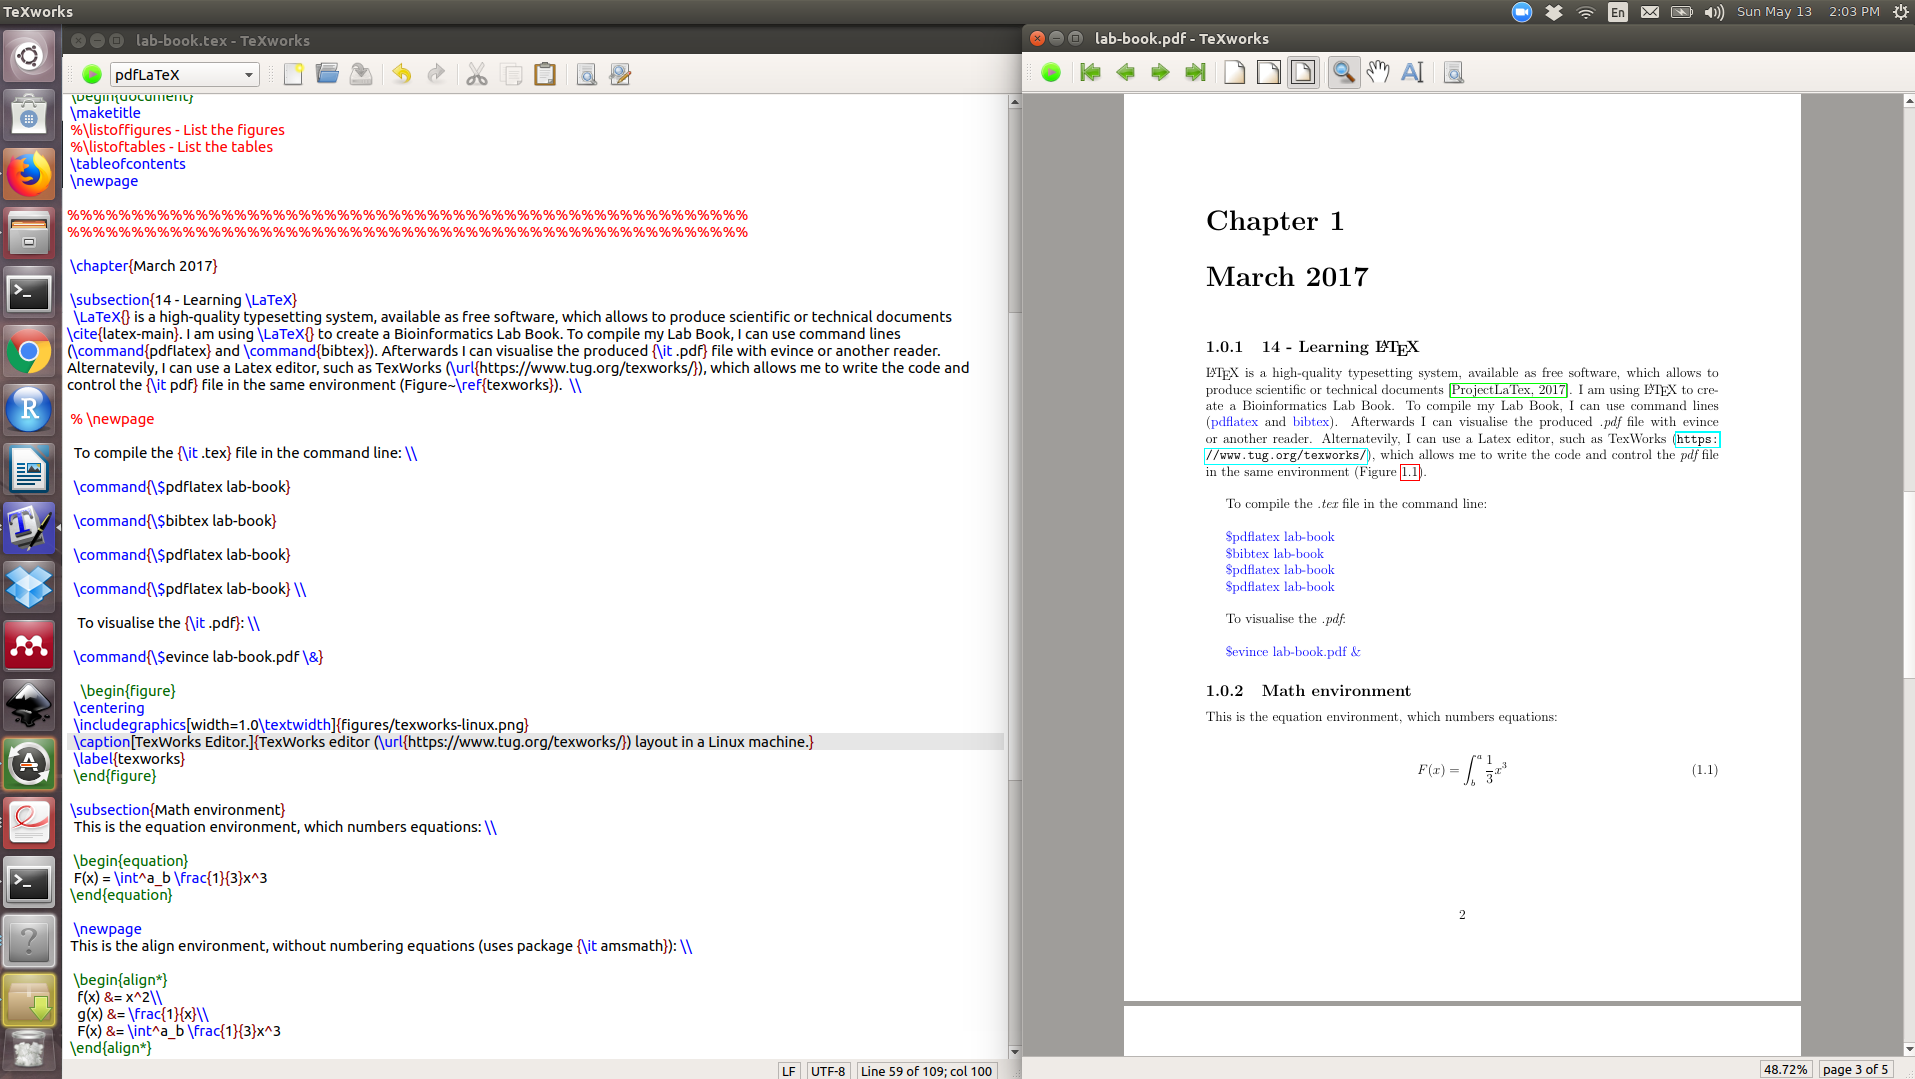
\includegraphics[width=1.0\textwidth]{figures/texworks-linux.png} 
  \caption[TexWorks Editor.]{TexWorks editor (\url{https://www.tug.org/texworks/}) layout in a Linux machine.}
  \label{texworks} 
  \end{figure}
  
 \subsection{Math environment}
  This is the equation environment, which numbers equations: \\
  
  \begin{equation}
  F(x) = \int^a_b \frac{1}{3}x^3
 \end{equation}
 
  \newpage
 This is the align environment, without numbering equations (uses package {\it amsmath}): \\
 
  \begin{align*}
   f(x) &= x^2\\
   g(x) &= \frac{1}{x}\\
   F(x) &= \int^a_b \frac{1}{3}x^3
 \end{align*}
 
  \subsection{15 - Short-term project proposal}
 Some text here. Incluing and referencing a table (table~\ref{table1}).
 
 \begin{itemize}
\item First numbered list item
\item Second numbered list item
\end{itemize}

\begin{table}[!htb]
  \caption{table0}
  \centering
  \begin{tabular}{ccc}
  \hline 
       species&changes&score \\
  \hline
       Macaque&4&0.0 \\
       Human&2&14.9 \\
       Orangutan&0&0.0 \\
       Pan&0&0.0 \\
       Gorilla&0&0.0 \\
  \hline
  \end{tabular}
  \label{table1}
 \end{table}

\chapter{Creation of data base of metagenomes and genomes}
\section{28}
\subsection{Bibliographic search for genomes}
Found a new possibility of phyla list. Because of this, there are four possibilities of list of microorganisms phyla, one of them, the SILVA database, is based in RNA sequences:
\begin{itemize}
\item The list of Prokariotic names with stading nomenclature \url{http://www.bacterio.net/-classifphyla.html}
\item SILVA database LSU(large subunit of ribosome) \url{https://www.arb-silva.de/browser/lsu/}
\item SILVA database SSU(small subunit of ribosome) \url{https://www.arb-silva.de/browser/ssu/}
\item PATRIC GENOMES \url{https://www.patricbrc.org/view/Taxonomy/2#view_tab=taxontree}
 \end{itemize}

The list of articles used until now is:
\begin{itemize}
\item 10.1038/nature14486
\item 10.1038/ismej.2013.111
\item 10.1038/ismej.2013.174
\item 10.1038/ismej.2016.43
\item 10.1038/nature12352
\item 10.1038/nature14486
\item 10.1038/nature21031
\item 10.1038/ismej.2015.233
\item 10.1038/ncomms13219
\item 10.1073/pnas.0801980105
\item 10.1111/1462-2920.13362
\item 10.1126/science.1132690
\item 10.1186/s40168-015-0077-6
\end{itemize}

\clearpage
\newpage
The list os correspondent phyla and articles is above\:

\begin{center}
\begin{longtable}{ccc}
\caption{table 1}\\
\hline
  DOI&Phylum\\
\hline
10.1038/nature14486	&	Candidatus Falkowbacteria	\\
10.1038/nature14486	&	Candidatus Kuenenbacteria	\\
10.1038/nature14486	&	Candidatus Magasanikbacteria	\\
10.1038/nature14486	&	Candidatus Uhrbacteria	\\
10.1038/nature14486	&	Candidatus Moranbacteria	\\
10.1038/nature14486	&	Candidatus Azambacteria	\\
10.1038/nature14486	&	Candidatus Yanofskybacteria	\\
10.1038/nature14486	&	Candidatus Jorgensenbacteria	\\
10.1038/nature14486	&	Candidatus Wolfebacteria	\\
10.1038/nature14486	&	Candidatus Giovannonibacteria	\\
10.1038/nature14486	&	Candidatus Nomurabacteria	\\
10.1038/nature14486	&	Candidatus Campbellbacteria	\\
10.1038/nature14486	&	Candidatus Adlerbacteria	\\
10.1038/nature14486	&	Candidatus Kaiserbacteria	\\
10.1038/nature14486	&	C. S. yataiensis	\\
10.1038/nature14486	&	Pacebacteria	\\
10.1038/nature14486	&	Candidatus Collierbacteria	\\
10.1038/nature14486	&	Candidatus Beckwithbacteria	\\
10.1038/nature14486	&	Candidatus Roizmanbacteria	\\
10.1038/nature14486	&	Candidatus Saphirobacteria	\\
10.1038/nature14486	&	Candidatus Amesbacteria	\\
10.1038/nature14486	&	Candidatus Woesebacteria	\\
10.1038/nature14486	&	Candidatus Gottesmanbacteria	\\
10.1038/nature14486	&	Candidatus Levybacteria	\\
10.1038/nature14486	&	Candidatus Daviesbacteria	\\
10.1038/nature14486	&	Candidatus Curtissbacteria	\\
10.1038/nature14486	&	WWE3	\\
10.1038/nature14486	&	CPR3	\\
10.1038/nature14486	&	WS6	\\
10.1038/nature14486	&	Candidatus Berkelbacteria	\\
10.1038/nature14486	&	Candidatus Peregrinibacteria	\\
10.1038/nature14486	&	Candidatus Gracilibacteria	\\
10.1038/nature14486	&	CPR2	\\
10.1038/nature14486	&	Kazan	\\
10.1038/nature14486	&	Saccharibacteria (TM7)	\\
10.1038/nature14486	&	SR1	\\
10.1038/ncomms13219	&	Candidatus Kerfeldbacteria 	\\
10.1038/ncomms13219	&	Candidatus Komeilibacteria	\\
10.1038/ncomms13219	&	Candidatus Andersenbacteria 	\\
10.1038/ncomms13219	&	Candidatus Ryanbacteria	\\
10.1038/ncomms13219	&	Candidatus Niyogibacteria 	\\
10.1038/ncomms13219	&	Candidatus Tagabacteria 	\\
10.1038/ncomms13219	&	Candidatus Terrybacteria 	\\
10.1038/ncomms13219	&	Candidatus Vogelbacteria	\\
10.1038/ncomms13219	&	Candidatus Zambryskibacteria 	\\
10.1038/ncomms13219	&	Candidatus Taylorbacteria	\\
10.1038/ncomms13219	&	Candidatus Sungbacteria	\\
10.1038/ncomms13219	&	Candidatus Brennerbacteria 	\\
10.1038/ncomms13219	&	Candidatus Spechtbacteria 	\\
10.1038/ncomms13219	&	Candidatus Staskawiczbacteria 	\\
10.1038/ncomms13219	&	Candidatus Wildermuthbacteria	\\
10.1038/ncomms13219	&	Candidatus Portnoybacteria 	\\
10.1038/ncomms13219	&	 Candidatus Woykebacteria 	\\
10.1038/ncomms13219	&	Candidatus Blackburnbacteria 	\\
10.1038/ncomms13219	&	Candidatus Chisholmbacteria 	\\
10.1038/ncomms13219	&	Candidatus Buchananbacteria	\\
10.1038/ncomms13219	&	Candidatus Jacksonbacteria 	\\
10.1038/ncomms13219	&	Candidatus Veblenbacteria	\\
10.1038/ncomms13219	&	Candidatus Nealsonbacteria 	\\
10.1038/ncomms13219	&	Candidatus Colwellbacteria 	\\
10.1038/ncomms13219	&	Candidatus Liptonbacteria 	\\
10.1038/ncomms13219	&	Candidatus Harrisonbacteria 	\\
10.1038/ncomms13219	&	Candidatus Yonathbacteria 	\\
10.1038/ncomms13219	&	Candidatus Lloydbacteria	\\
10.1038/ncomms13219	&	Candidatus Abawacabacteria	\\
10.1038/ncomms13219	&	Candidatus Doudnabacteria	\\
10.1038/ismej.2013.111	&	Candidatus Poribacteria	\\
10.1111/1462-2920.13362	&	Candidatus Desantisbacteria	\\
10.1038/nature12352	&	Candidatus Omnitrophica	\\
10.1038/nature12352	&	Candidatus Aminicenantes	\\
10.1126/science.1132690	&	Candidatus Micrarchaeota	\\
10.1038/nature14486	&	Candidatus Magasanikbacteria	\\
10.1073/pnas.0801980105	&	Candidatus Korarchaeota	\\
10.1038/nature12352	&	Candidatus Fervidibacteria	\\
10.1038/nature12352	&	Candidatus Aenigmarchaeota	\\
10.1038/ismej.2016.43	&	Candidatus Fermentibacteria	\\
10.1038/ismej.2013.174	&	Candidatus Bathyarchaeota	\\
10.1016/j.cub.2015.01.014	&	Candidatus Woesearchaeota	\\
10.1016/j.cub.2015.01.014	&	Candidatus Kryptonia	\\
10.1038/nature12352	&	Candidatus Diapherotrites	\\
10.1038/nature12352	&	Candidatus Latescibacteria	\\
10.1038/nature21031 10.1038/ismej.2015.233	&	Candidatus Thorarchaeota	\\
10.1038/ncomms13219	&	Candidatus Lindowbacteria	\\
10.1038/nature12352	&	Candidatus Parvarchaeota	\\
10.1038/nature12352	&	Candidatus Cloacimonetes	\\
10.1038/nature12352	&	Candidatus Hydrogenedentes	\\
10.1038/nature12352	&	Candidatus Acetothermia	\\
10.1038/nature12352	&	Candidatus Nanohaloarchaeota	\\
10.1038/ncomms13219	&	Candidatus Eisenbacteria	\\
10.1186/s40168-015-0077-6	&	candidate division WOR-3	\\
10.1038/nature21031 &  Lokiarchaeota \\
10.1038/nature21031 & Odinarchaeota \\
10.1038/nature21031 & Heimdallarchaeota \\

 \hline
  \end{longtable}
\end{center}

\section{28}

\subsection{Bibliographic search for metagenomes}
The reserarch for coral metagenomes started last year. The actual list is:

\begin{center}
\begin{longtable}{c}
\caption{table 1}\\
\hline
  IDs\\
\hline
mgm4440319.3\\
mgm4440370.3\\
mgm4440371.3\\
mgm4440372.3\\
mgm4440373.3\\
mgm4440374.3\\
mgm4440375.3\\
mgm4440376.3\\
mgm4440377.3\\
mgm4440378.3\\
mgm4440379.3\\
mgm4440380.3\\
mgm4440381.3\\
mgm4445755.3\\
mgm4445756.3\\
mgm4480739.3\\
mgm4480740.3\\
mgm4480741.3\\
mgm4480748.3\\
mgm4480750.3\\
mgm4487909.3\\
mgm4487910.3\\
mgm4487911.3\\
mgm4516541.3\\
mgm4516694.3\\
mgm4653307.3\\
mgm4694757.3\\
mgm4694758.3\\
mgm4694759.3\\
mgm4694760.3\\
SRR1275409\\
SRR1275449\\
SRR1283349\\
SRR1283371\\
SRR1283377\\
SRR1283433\\
SRR1283435\\
SRR1283437\\
SRR1286223\\
SRR1286225\\
SRR1286226\\
SRR1286227\\
SRR1286229\\
SRR1286232\\
SRR1822488\\
SRR1822516\\
SRR3499156\\
SRR3569370\\
SRR3694369\\
SRR3694370\\
SRR3694371\\
SRR3694372\\
SRR5215424\\
SRR5215454\\
SRR5215455\\
SRR5215456\\
SRR5215457\\
SRR5215458\\
SRR5215462\\
SRR5605611\\
 \end{longtable}
\end{center}


I found these metagenomes in the article: "Metagenomic analysis reveals a green sulfur bacterium as a potential coral symbiont"

\begin{center}
\begin{longtable}{c}
SRR2937345\\
SRR2937346\\
SRR2937347\\
SRR2937348\\
SRR2937349\\
SRR2937350\\
SRR2937351\\
SRR2937352\\
SRR2937353\\
SRR2937354\\
SRR2937355\\
SRR2937356\\
 \end{longtable}
\end{center}


Espécie: Platygyra carnosa
Healthy

I found other metagenomes of coral from article\: doi \"10.3389/fmars.2018.00101\"
I uptated the file pmc\_results\_1.txt in the repository Lab\_book. I continue to look the articles in results. 
Estou atualizando a lista pmc\_results\_2.txt
Na pesquisa bibliografica\, olhando o título ja me faz perceber se devo descartar e olhar. E olho aqueles que marquei para olhar. Ao olhar, leio o resumo procurando por metodos.  E vou para os metodos do artigo para checar.
Checking the sizes of metagenomes files. The mg-rast metagenomes base have 72 Gb. 

The pipeline of bioinformatic is different for MG\-RAST and NCBI.
The size of NCBI should be superestimated, because the ncbi says the file size of sra file, but most of them is paired-end metagenomes, so when we apply fastq-dump, its generate two files fastq. 

\subsection{Amostras do MG-RAST indicadas pelo professor e Miguel}
Na reuniao feita em 30 de outubro, o professor e Miguel indicaram amostras existentes de Madracis para serem analisadas. O artigo é entitulado: "Turbulence-driven shifts in holobionts and planktonic microbial assemblages in St. Peter and St. Paul Archipelago, Mid-Atlantic Ridge, Brazil". DOI: 10.3389/fmicb.2015.01038. Amostras inclusas: 
\begin{itemize}
\item mgm4486661.3
\item mgm4486662.3
\item mgm4486663.3
\item mgm4486664.3
\item mgm4486665.3
\item mgm4486666.3
\item mgm4486667.3
\item mgm4486668.3
\item mgm4486669.3
\end{itemize}
O estado de saude dessas amostras nao esta claramente indicado no MG-RAST, mas pelo nome da amostra. No artigo, as amostras de Madracis branqueadas estão nomeadas com madble.

O professor indicou procurar pelo laboratorio do professor Alexandre Rosado, para encontrar mais amostras de metagenomas de corais feitas no Brasil, especificamente nos trabalho de Raquel Peixoto (nao estava encontrando antes porque pensava que o nome era Raquel Rosado). Indo em seu perfil no google academico, utilizei o recurso de ctrl f, pesquisando por coral. Os trabalhos que continham 'coral' no título não são de metagenoma. 


\chapter{Download of metagenomes}
\section{Download of mg-rast files} 
Espaço no SDU
Disponível para o ebiodiv: 10Tb
Bia: 5Tb
Rilquer: 2T
Remanescente: 3Tb

\begin{tcolorbox}[width=6.3in]
 \scriptsize 
 - Working folder: \textit{scratch/ebiodiv/leticia.cavalcante/mg\_rast}
 \end{tcolorbox}

I insert the list of metagenomes in the files before using it. After this, I used the following command line:

\begin{tcolorbox}[width=6.3in]
 \scriptsize 
 - Command: \textit{nohup bash download\_curl\_mgrast\_corais.sh > download\_curl\_mgrast\_corais.nohupout \&}
 \end{tcolorbox}

\section{Download of NCBI metagenomes}
I use the script download\_sra\_wget\_corais.sh, libs folder. I used the wget, because the curl is getting some problem in SDU.
I noted that the size of the files is different:


\begin{table}[!htb]
  \caption{Comparing sizes of files}
  \centering
  \begin{tabular}{ccc}
  \hline 
       ID of metagenome&the size in NCBI site&size of file in SDU\\
  \hline
	SRR6785058&317.00 Mb&318M\\
	SRR6785057&364.00 Mb&365M\\
	SRR6785056&560.00 Mb&561M\\
	SRR6785055&624.00 Mb&625M\\
  \hline
  \end{tabular}
  \label{table2}
 \end{table}

So I checked the others files:

\begin{table}[H]
  \caption{Comparing sizes of files 2}
  \centering
  \begin{tabular}{cccc}
  \hline 
       ID of metagenome&the size in NCBI site&size of file in SDU&size of cleanned file\\
  \hline
	mgm4440319.3.299.1&30M&29.1 MB&28M\\
	mgm4440370.3.299.1&3,6M&3.5 MB&3,5M\\
	mgm4440371.3.299.1&5,0M&4.9 MB&4,8M\\
	mgm4440372.3.299.1&6,0M&6.0 MB&5,9M\\
	mgm4440373.3.299.1&6,2M&6.1 MB&6,0M\\
	mgm4440374.3.299.1&4,1M&4.1 MB&4,0M\\
	mgm4440375.3.299.1&3,8M&3.7 MB&3,7M\\
	mgm4440376.3.299.1&3,9M&3.9 MB&3,8M\\
	mgm4440377.3.299.1&3,5M&3.5 MB&3,4M\\
	mgm4440378.3.299.1&6,2M&6.2 MB&6,1M\\
	mgm4440379.3.299.1&7,0M&7.0 MB&6,9M\\
	mgm4440380.3.299.1&5,2M&5.2 MB&5,2M\\
	mgm4440381.3.299.1&6,4M&6.4 MB&6,4M\\
	mgm4445755.3.299.1&158M&157.0 MB&155M\\
	mgm4445756.3.299.1&150M&149.9 MB&147M\\
	mgm4480739.3.299.1&8,0M&7.9 MB&7,9M\\
	mgm4480740.3.299.1&12M&11.3 MB&12M\\
	mgm4480741.3.299.1&8,5M&8.5 MB&8,5M\\
	mgm4480742.3.299.1&10M&12.9 MB&10M\\
	mgm4480743.3.299.1&15M&10.0 MB&14M\\
	mgm4484839.3.299.1&13M&14.1 MB&13M\\
	mgm4487909.3.299.1&17M&16.5 MB&17M\\
	mgm4487910.3.299.1&36M&35.6 MB&36M\\
	mgm4487911.3.299.1&12M&11.4 MB&12M\\
	mgm4516541.3.299.1&161M&160.2 MB&163M\\
	mgm4516694.3.299.1&193M&192.9 MB&193M\\
	mgm4653307.3.299.1&17M&16.0 MB&17M\\
	mgm4694757.3.299.1&1,9G&1.8 GB&1,9G\\
	mgm4694758.3.299.1&2,2G&2.1 GB&2,2G\\
	mgm4694759.3.299.1&1,7G&1.7 GB&1,8G\\
	mgm4694760.3.299.1&592M&1.6 GB&597M\\
  \hline
  \end{tabular}
  \label{table3}
 \end{table}

A Bia me informou que o SDU arrendonda os valores de tamanho dos arquivos, entao até o momento nao
tive problemas com o download dos arquivos do mg\_rast

\subsection{Amostras indicadas por Miguel na reuniao de 30 de novembro}
Fiz um loop para baixar as amostras chamado: loop\_download\_6\_november.sh, funcionou no computador local, mas nao no servidor por algum motivo ligado a internet. Por isso, fiz o download das amostras no computador local e as transferi para o cluster Atlantico.


\chapter{Format Conversion of NCBI metagenomes}
 
Adaptei o script da Bia para fazer a conversao do dos arquivos .sra\\
Inicialmente submeti apenas um na cpu\_dev para testar:\\ 

\begin{tcolorbox}[width=5.3in]
 \scriptsize 
\normalsize  Script: \textit{teste\_slurm\_job\_fastq\_dump\_corais.sh}\\
\normalsize  Numero do job: \textit{220896}
 \end{tcolorbox}

Deu certo. \\
O Rilquer me ajudou a criar um script que cria jobs de anotacao com o kraken2 para cada dois metagenomas. \\
O nome do script é 'creatijobfile.sh', ele unirá dois scripts: 'header' e 'ending' \\
Adaptei para criar jobs do fastq-dump para cada 2 arquivos .sra, haja visto que não tenho uma boa ideia do quanto cada fastq-dump demorará. \\

Jobs submetidos dia 27/09/2018:
\begin{itemize}
\item job\_0.sh - job 221475
\item job\_100.sh - job 221476
\item job\_102.sh - job 221477
\item job\_104.sh - job 221478
\item job\_106.sh - job 221480
\item job\_108.sh - job 221481
\item job\_10.sh - job 221482
\item job\_110.sh - job 221483
\item job\_112.sh - job 221484
\item job\_114.sh - job 221485
\item job\_116.sh - job 221486
\item job\_118.sh - job 221487
\item job\_120.sh - job 221488
\item job\_122.sh - job 221489
\item job\_124.sh - job 221490
\item job\_126.sh - job 221493
\item job\_12.sh - job 221495
\end{itemize}

Jobs submetidos dia 09/10/2018:
\begin{itemize}
\item job\_14.sh - slurm 226902
\item job\_16.sh - slurm 226903
\item job\_18.sh - slurm 226904
\item job\_20.sh - slurm 226905
\item job\_22.sh - slurm 226906
\item job\_24.sh - slurm 226907
\item job\_26.sh - slurm 226908
\item job\_28.sh - slurm 226909
\item job\_2.sh - slurm 226910
\item job\_30.sh - slurm 226911
\item job\_32.sh - slurm 226912
\end{itemize}

Jobs submetidos dia 19/10/2018:
\begin{itemize}
\item job\_34.sh - slurm 231744
\item job\_36.sh - slurm 231745
\item job\_38.sh - slurm 231746
\item job\_40.sh - slurm 231747
\item job\_42.sh - slurm 231748
\item job\_44.sh - slurm 231749
\item job\_46.sh - slurm 231750
\item job\_48.sh - slurm 231751
\item job\_4.sh - slurm 231752
\item job\_50.sh - slurm 231753
\item job\_52.sh - slurm 231754
\item job\_54.sh - slurm 231755
\end{itemize}

\subsection{Taxonprofiling}
Essa subsecao foi escrita apos o Rilquer construir um script que unifica as etapas de bioinformatica em um script unico.
Com script do Rilquer chamando Taxonprofiling, todas as etapas de bioinformatica estão unidas em um so script. Os jobs acimas estão guardados, mas com a utilizacao do script que o Rilquer construiu, as amostras estao sendo analisadas no Atlantico, cluster da UFBA

\chapter{Adaptacao dos identificadores}

Esse passo fez-se necessário nas análises anteriores, pois quando eu fazia a limpeza, os arquivos de outputs que saiam eram apenas os singletons. 
The output files were named as SRAXXX\_good\_singletons\_1 and SRAXXX\_good\_singletons\_2 and there aren’t any other output files beyond these and the files with bad sequences. 
O Pablo fez a seguinte sugestão:

%cat SRR1275409\_pass\_1.fastq | sed -r 's/(SRR1275409.[0-9]+).([0-9]+)/\1\_left/\' > SRR1275409\_pass\_1.corr.fastq

%cat SRR1275409\_pass\_2.fastq | sed -r 's/(SRR1275409.[0-9]+).([0-9]+)/\1\_right/\' > SRR1275409\_pass\_2.corr.fastq

\begin{lstlisting}[breaklines]
cat SRR1275409_pass_1.fastq | sed -r 's/(SRR1275409.[0-9]+).([0-9]+)/\1_left/' > SRR1275409_pass_1.corr.fastq

cat SRR1275409_pass_2.fastq | sed -r 's/(SRR1275409.[0-9]+).([0-9]+)/\1_right/' > SRR1275409_pass_2.corr.fastq
\end{lstlisting}

\chapter{Quality filter}
This step is only required for NCBI metagenomes. The command line was proposed by Bia:
\begin{itemize}
\item trim\_qual\_left 25
\item trim\_qual\_right 25
\end{itemize}

\subsection{Taxonprofiling}
Essa subsecao foi escrita apos o Rilquer construir um script que unifica as etapas de bioinformatica em um script unico.
A etapa do quality filter foi modificada pelo Rilquer, apos ele insistir com o professor sobre qual seriam os melhores parametros de qualidade. 

Segue criterios de qualidade:
\begin{itemize}
\item min\_qual\_score 13
\item trim\_qual\_left 13
\item trim\_qual\_right 13
\end{itemize}

Linha parcial abaixo: 

\begin{lstlisting}[breaklines]
-min_qual_score 13 -trim_qual_left 13 -trim_qual_right 13 -ns_max_n 2
\end{lstlisting}


\chapter{Uniformity filter (size and N bases)}
\section{Command line}
Parameters:
\begin{itemize}
\item min\_len 80 
\item ns\_max\_p 2 
\item out\_format 1
\end{itemize}

\begin{tcolorbox}[width=6.3in]
 - Command: \textit{nohup bash slurm\_job\_prinseq\_single\_corais\_FASTA.bash \&> slurm\_prinseq\_corais.out \&}
 \end{tcolorbox}

Deu erro o job\:
nohup: ignorando entrada

\begin{tcolorbox}[width=6.3in]
 \scriptsize 
Location of PRINSEQ dir and scripts: /scratch/app/prinseq/0.20.4/bin
srun\: Warning: can't run 1 processes on 21 nodes, setting nnodes to 1
srun\: Requested partition configuration not available now
srun\: job 212425 queued and waiting for resources
srun\: Force Terminated job 212425
srun\: Job has been cancelled
srun\: error: Unable to allocate resources: No error
srun\: Warning: can't run 1 processes on 21 nodes, setting nnodes to 1
srun\: Requested partition configuration not available now
srun\: job 212428 queued and waiting for resources
srun\: Force Terminated job 212428
srun\: Job has been cancelled
\end{tcolorbox}


 \begin{figure}[H]
  \centering 
  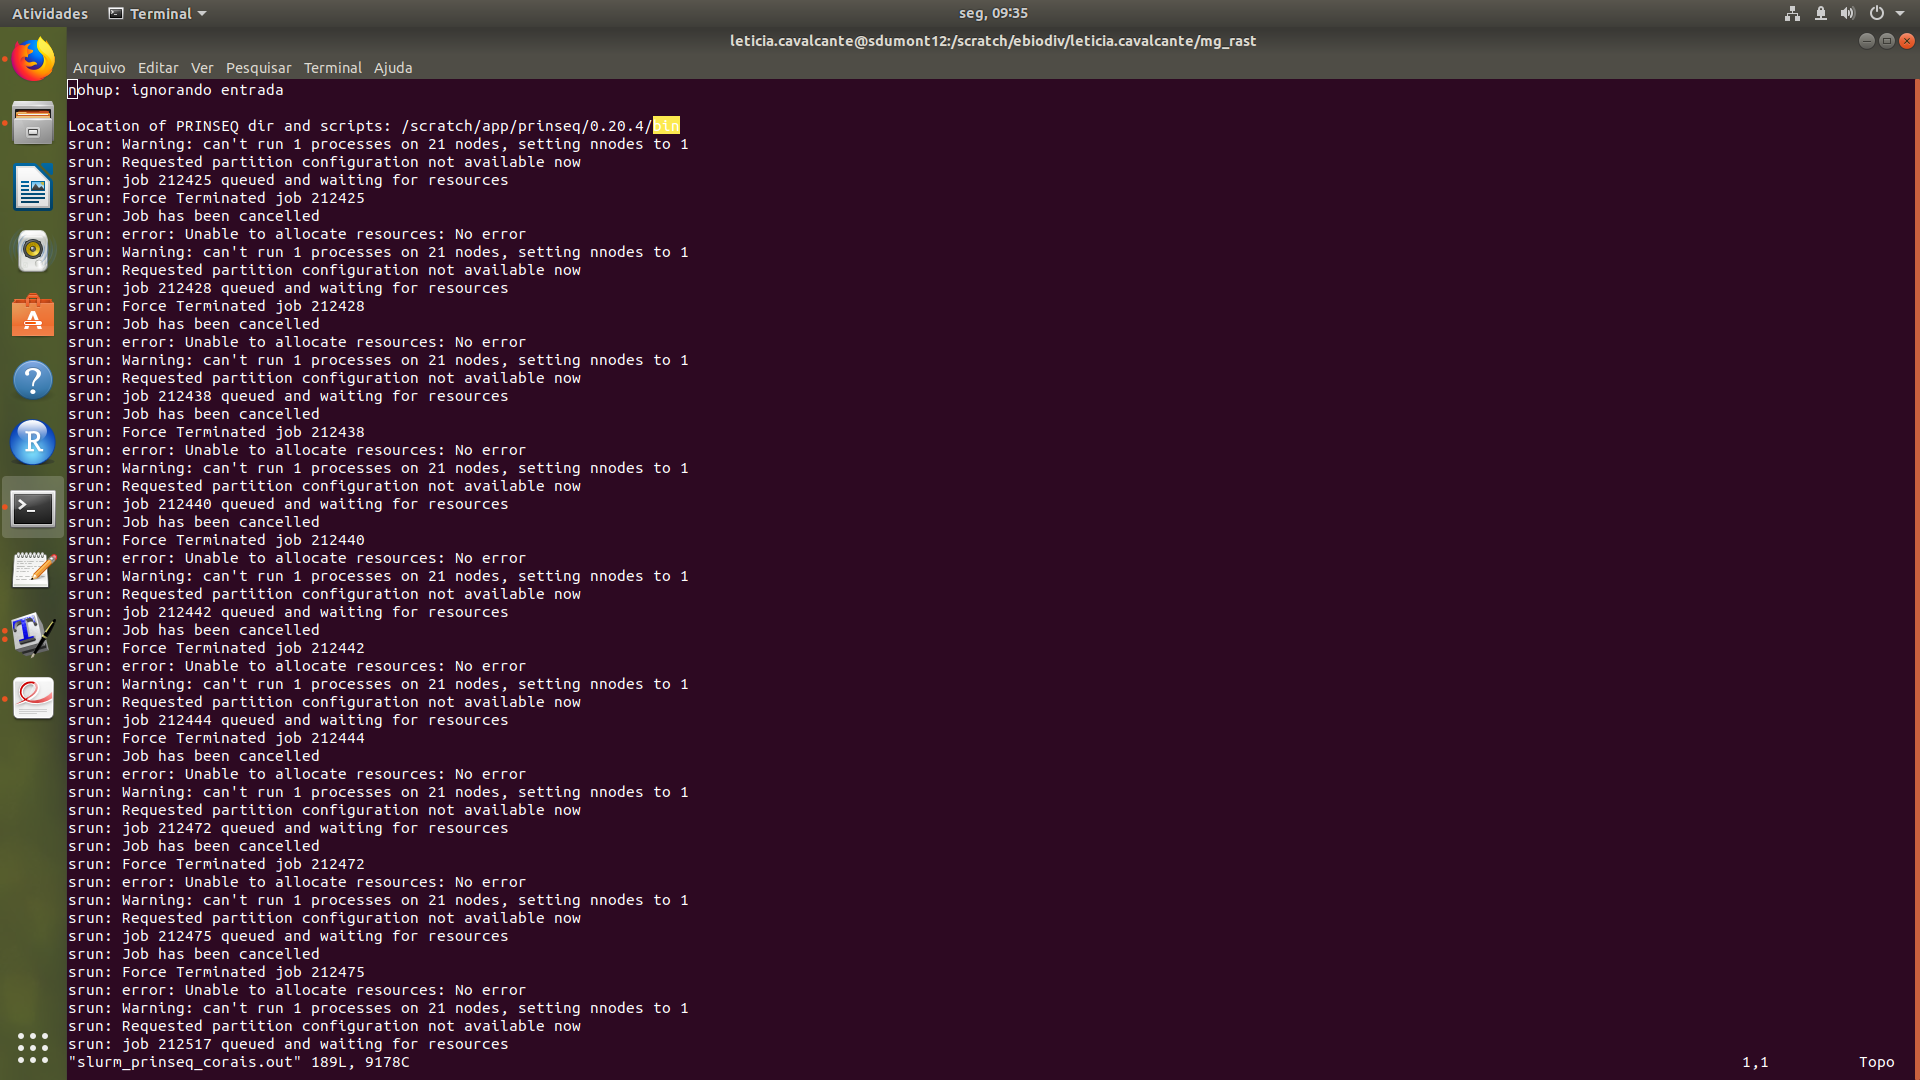
\includegraphics[width=1.0\textwidth]{figures/Captura-2018-09-10 09-35-27.png}
  \caption{Erro no job no SDU}
 \end{figure}

Ressubmeti o job com:

\begin{tcolorbox}[width=6.3in]
- Command: \textit{sbatch slurm\_job\_prinseq\_single\_corais\_FASTA.bash}
\end{tcolorbox}

\subsection{Utilizacao do Taxonprofiling}
Essa subsecao foi escrita apos o Rilquer construir um script que unifica as etapas de bioinformatica em um script unico.
Os criterios foram modificados para:
\begin{itemize}
\item -min\_len 50
\item -ns\_max\_n 2
\end{itemize}

\textbf{Linha total}:
\begin{lstlisting}[breaklines]
prinseq-lite -verbose -fastq ${OUTDIR}/fastqdump_output/${id}_pass_1.fastq -fastq2 ${OUTDIR}/fastqdump_output/${id}_pass_2.fastq -min_len 50 -min_qual_score 13 -trim_qual_left 13 -trim_qual_right 13 -ns_max_n 2 -out_format 1

\end{lstlisting}
 

\chapter{Profilling metagenomes}
\section{Mg-Rast metagenomes}
I used the following script in the following folder:

\begin{tcolorbox}[width=6.3in]
- Folder: \textit{scratch/ebiodiv/leticia.cavalcante/mg\_rast/filtered\_prinseq\_good}\\
- Command: \textit{sbatch slurm\_job\_kraken2\_corais.sh}
\end{tcolorbox}

The job doesn't work, o erro aparece na proxima figura

Ressubmeti o job, modificando a localizacao da DB do Kraken para a home do Rilquer. Numero do job: 216410
 \begin{figure}
  \centering 
  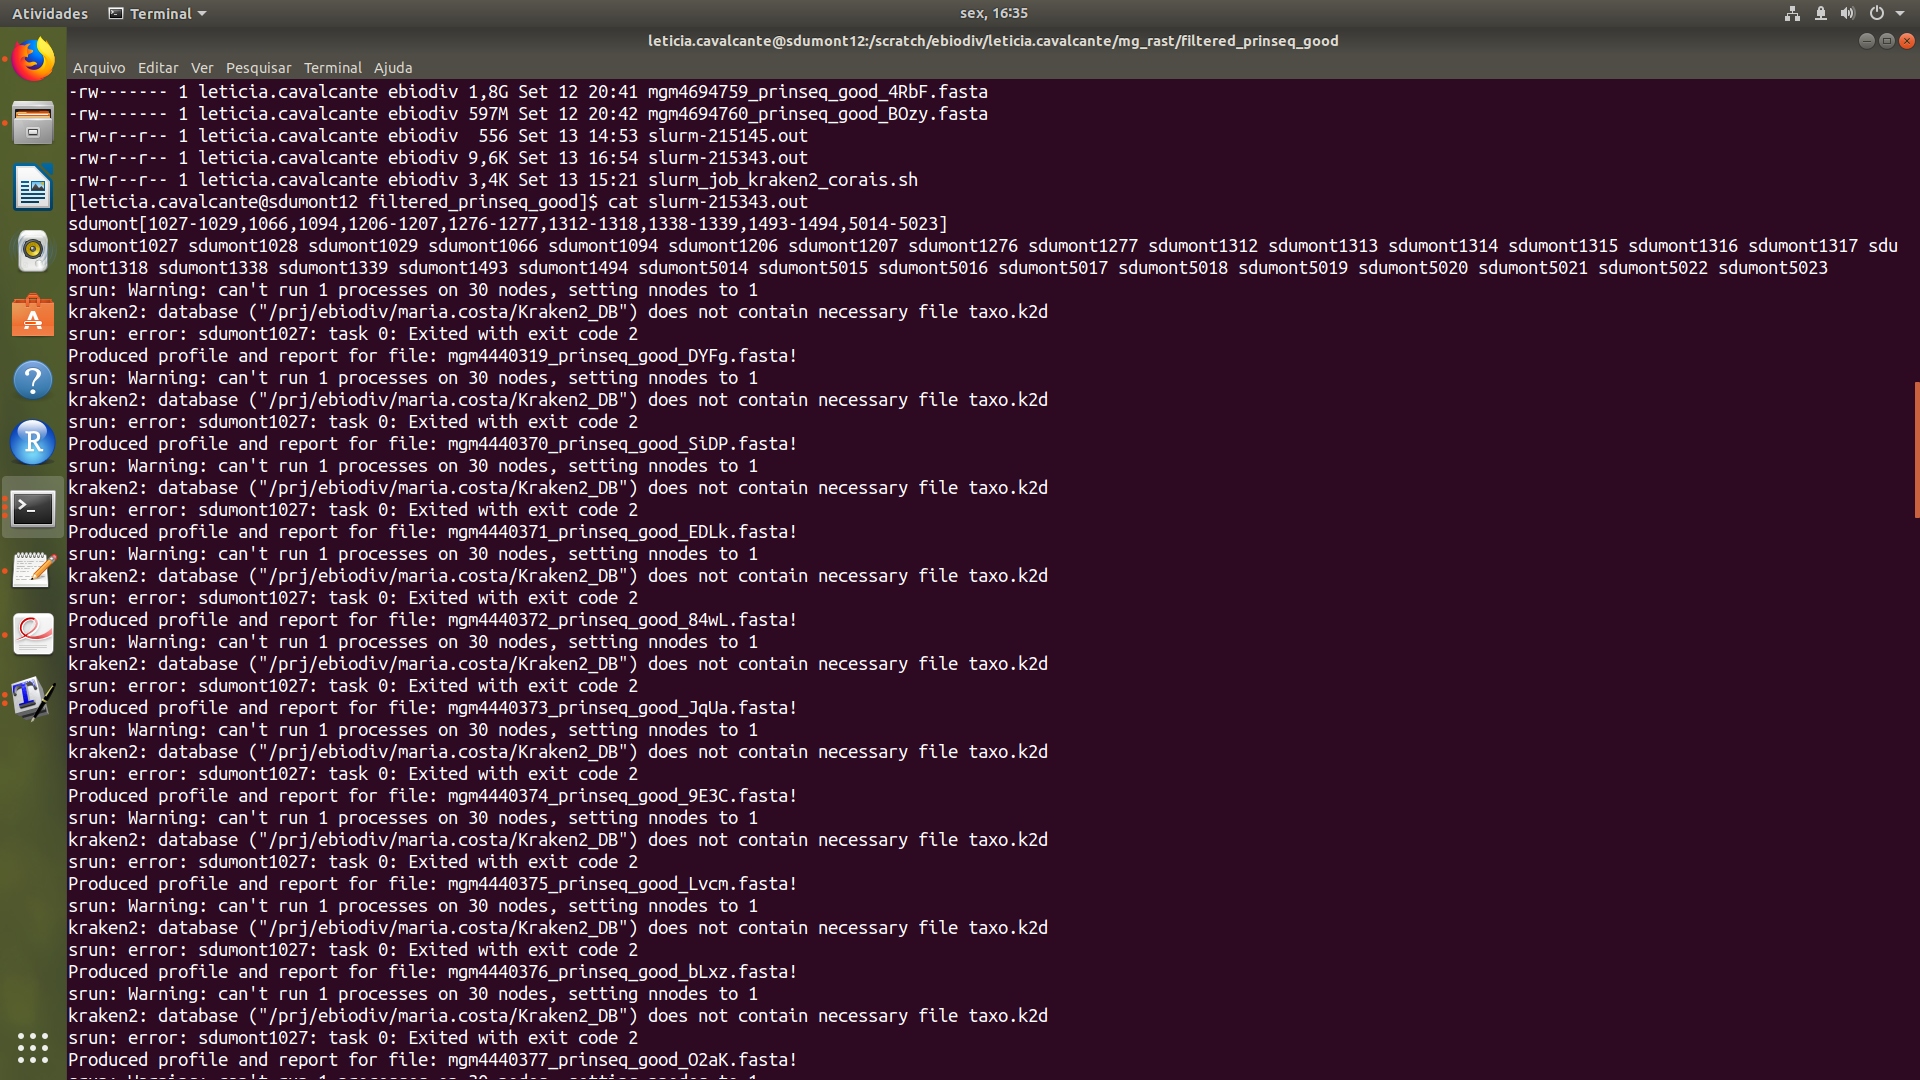
\includegraphics[width=1.0\textwidth]{figures/Captura2.png}
  \caption{2o erro no job no SDU}
 \end{figure} 

Esse problema foi resolvido modificando o endereco da base para o scratch do Rilquer.

\begin{figure}
  \centering 
  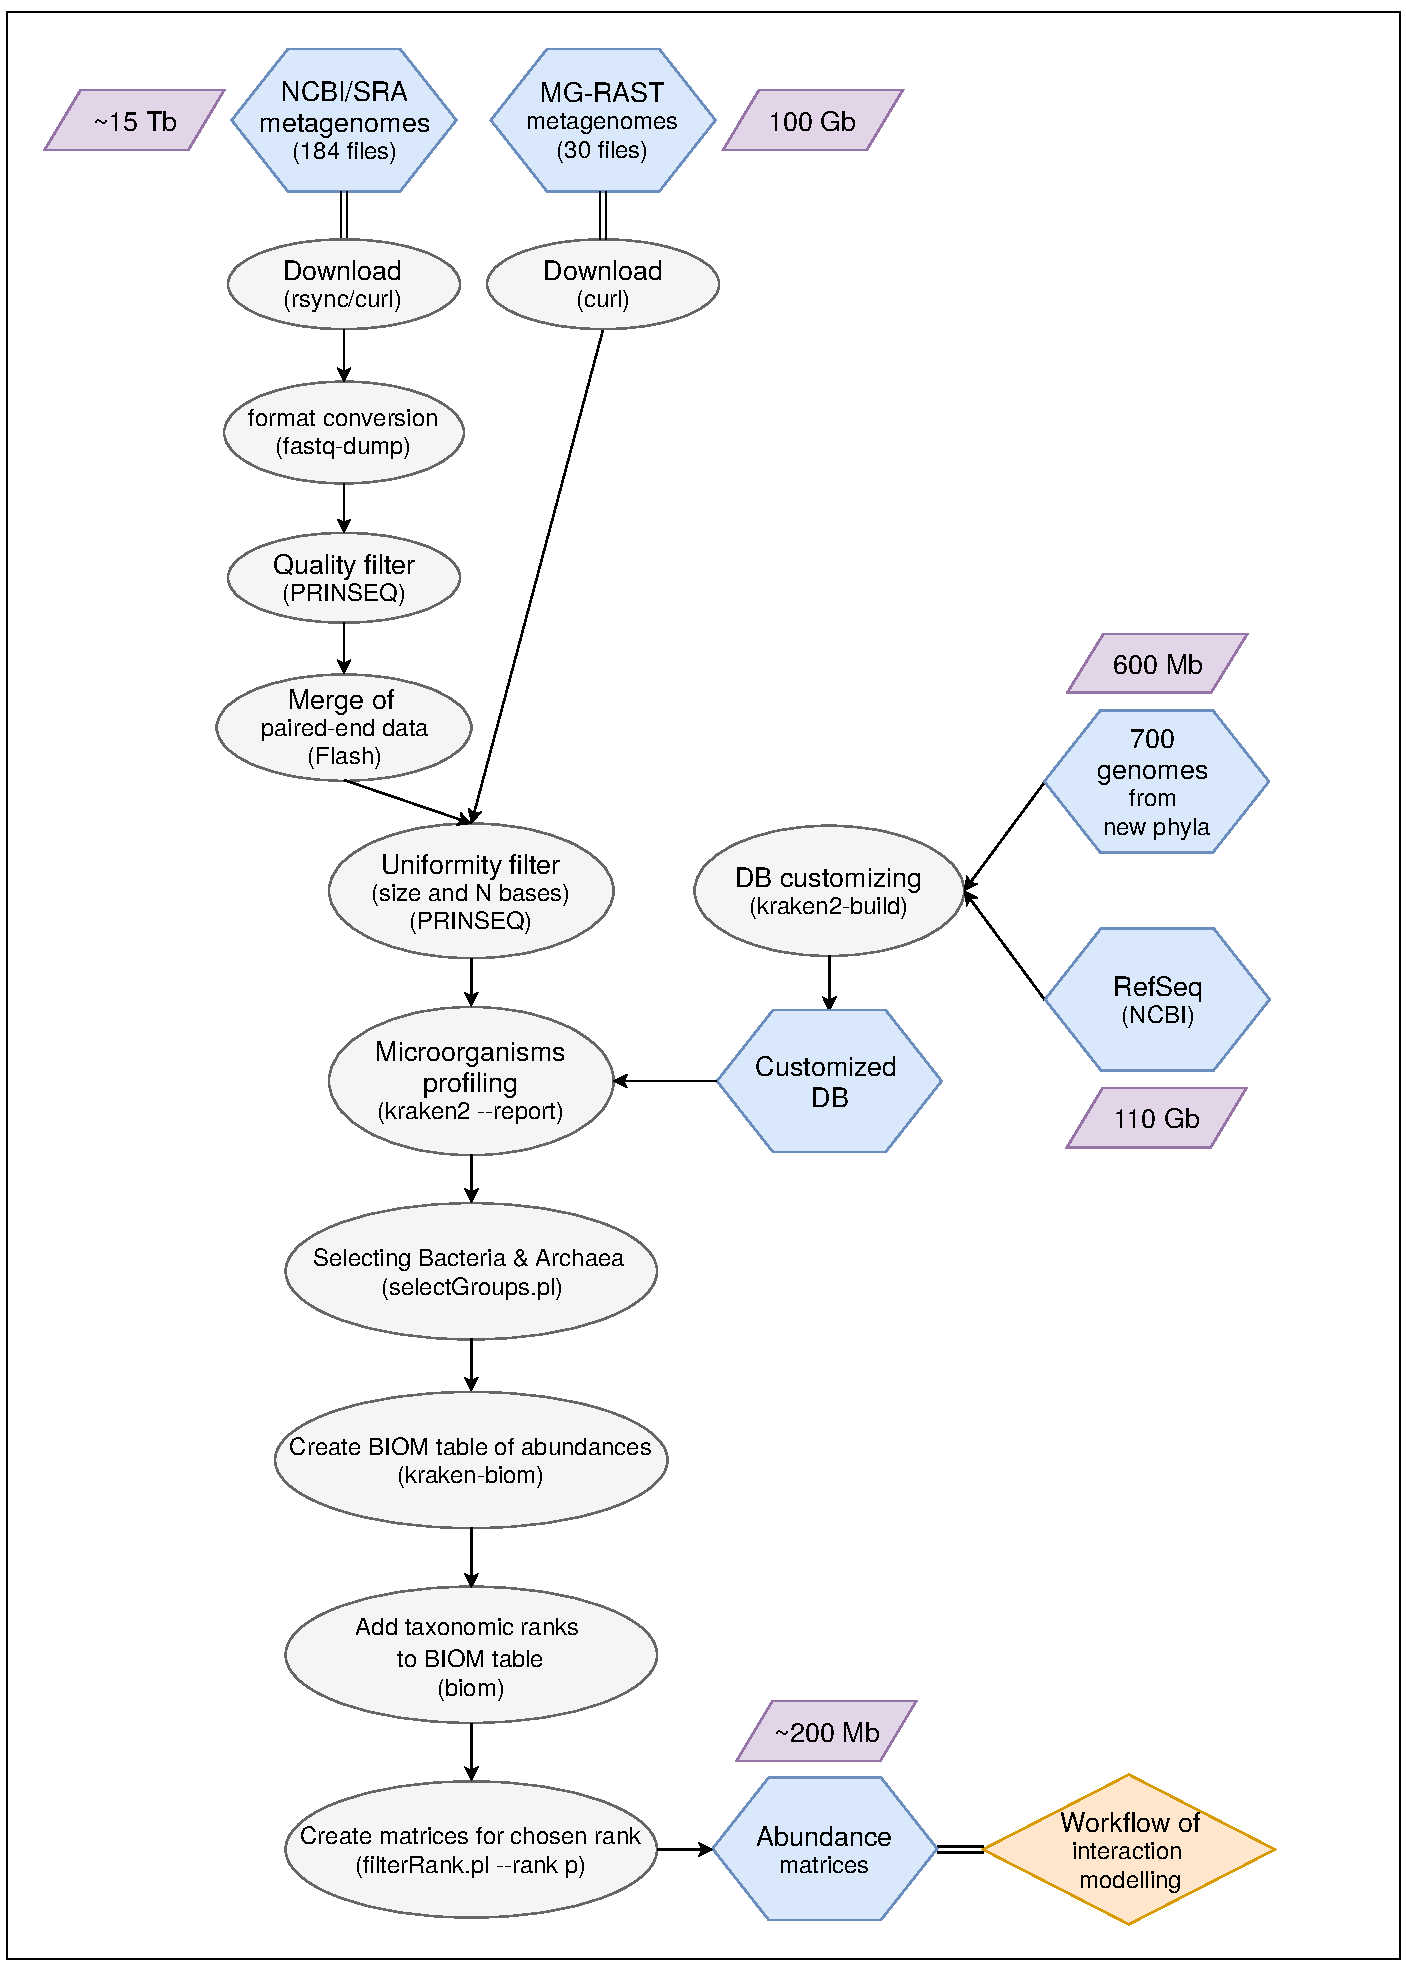
\includegraphics[width=0.9\textwidth]{figures/workflow-aquifers-reviewed_03-09-18.pdf}
  \caption{Pipeline of taxonomic annotation} 
  \end{figure}

\section{Kraken-biom}
Pasta onde está instalado kraken-biom: \\
/home/leticia/.local/bin

Para executar:
python2.7 .\/kraken-biom \\

Executar o help do kraken-biom: \\
kraken-biom -h \\

Abrir no vim o arquivo .bashrc e inserir: \\
export PATH=\$PATH:/home/leticia/.local/bin/kraken-biom \\

Executar o help do kraken-biom: \\
kraken-biom -h \\

 
Eu fiz um teste da etapa "Creation of BIOM table of abundances" da pipeline da bia com os seguintes passos:
Na pasta\: 
 /home/leticia/Documentos/libs/leticia\_profiling\_metagenomes: 

\begin{itemize}
\item kraken-biom selected\_file -o table.biom --max D --min P 
\item biom convert -i table.biom -o table.from\_biom\_with\_taxonomy.txt --to-tsv --header-key taxonomy 
\item perl filterRank.pl \-\-input table.from\_biom\_with\_taxonomy.txt --rank p > abundance.matrix 
\end{itemize}

\section{Teste com o kraken no scratch}
Linha de teste: \\
perl selectGroups.pl \-\-input mgm4440370\_prinseq\_good\_SiDP.fasta\_kraken.report --file\_groups groups.txt > selected\_file


\begin{tcolorbox}[width=6.3in]
- First Command: \textit{sbatch slurm\_job\_kraken2\_corais.sh}\\
- Second Command: \textit{\\
kraken2 --db /prj/ebiodiv/rilquer.silva/Serrapilheira \\
/Kraken2\_custom\_DB/ mgm4440370\_prinseq\_good\_SiDP.fasta \\
--output mgm4440370\_prinseq\_good\_SiDP.fasta\_kraken.profiled \\
--use-names --report mgm4440370\_prinseq\_good\_SiDP.fasta\_kraken.report}
\end{tcolorbox}

Ja testei o comando acima na home do SDU e agora no scratch

\newpage
\section{Profiling no Atlantico com a ajuda do Rilquer}
\subsection{MG RAST metagenomes}
O Rilquer fez um script que automatiza o processo, em que a limpeza e anotacao ocorrem simultanetamente. Fiz um teste com esse script para um metagenoma com a seguinte linha:

\begin{tcolorbox}[width=6.3in]
- Comand: \textit{taxonprofiling -s mgm4440378.3.299.1 -f MGRAST -k /home/pedro/Kraken2\_custom\_DB}\\
- Script: taxonprofiling\\
- Folder: /fsprofpedro/holobionts/mgrast\\
- Para chamar o script: taxonprofiling
\end{tcolorbox}

Sairam 4 outputs:
\begin{itemize}
\item mgm4440378\_kraken\_class
\item mgm4440378\_kraken\_output
\item mgm4440378\_kraken\_report
\item mgm4440378\_kraken\_unclass
\end{itemize}

De acordo com a pipeline da Bia, o arquivo a ser usado e o report. Teste a seguir com a pasta com os metagenomas do mg-rast inteiro:

\begin{tcolorbox}[width=6.3in]
-Comand: \textit{taxonprofiling -d /fsprofpedro/holobionts/mgrast -f MGRAST -k /home/pedro/Kraken2\_custom\_DB}\\
- Folder: /fsprofpedro/holobionts
\end{tcolorbox}

No email do Rilquer, vi que tenho que submeter o job para uma fila que não tem acesso ao fsprofpedro. Então criei uma pasta temporaria chamada mgrast\_temp, no home/pedro

\begin{tcolorbox}
- Job: \textit{profiling\_metagenomes\_corais\_mgrast.sh}\\
- Folder temporario em que as amostras foram copiadas: /home/pedro/mgrast\_temp \\
-Folder de submissao:  /home/pedro/
\end{tcolorbox}

Na pasta /fsprofpedro/holobionts, tem um exemplo de job chamado jobexample. Submissao:
\begin{tcolorbox}
-Folder de submissao: /home/pedro/mgrast\_temp \\
- Numero: 122296.atlantico\\
- Command: qsub profiling\_metagenomes\_corais\_mgrast.sh
\end{tcolorbox}

I have noticed that the files of abundance matrix is empty, I need to warn Rilquer. I had transferred the report files to this computer, to the following folder: /home/leticia/Documentos/dados/report\_atualizado\_23\_10\_2018.

Sequence of command lines:


\begin{tcolorbox}[width=6.7in]
- Folder: /home/leticia/Documentos/libs/leticia\_profiling\_metagenomes \\
Command 1: nohup  bash select\_groups\_perl\_corais.sh > select\_groups\_corais\_perl.nohupout \&

Command 2: biom convert -i table\_corais\_mg\_rast.biom -o table\_corais\_mg\_rast.from\_biom\_with\_taxonomy.txt --to-tsv --header-key taxonomy

Comman 3: perl filterRank.pl --input table\_corais\_mg\_rast.from\_biom\_with\_taxonomy.txt --rank p > abundance\_corais\_mgrast\_2.matrix
\end{tcolorbox}

Output gerado: \textbf{abundance\_corais\_mgrast\_2.matrix} . O output gerado foi modificado no R, transposto, colocado em porcentagem e com os detalhes de genero, especie e estado de saude e retirei a linha gerada quando transformei em data frame, com X1, X2 e etc. 

Coloquei para rodar novamente as amostras do MG-RAST para as matrizes de família serem geradas. Job: 123190.atlantico

\subsection{SRA metagenomes}
Originalmente, os arquivos estão no folder:\textbf {/fsprofpedro/holobionts/SRA}. O total de arquivos é 158764768. Para fazer o trabalho de fastq dump, limpeza e anotacao, os arquivos devem estar no seguinte folder:

\begin{tcolorbox}[width=6.3in]
- Folder: \textit{/home/pedro/holobionts\_temp/SRA} \\
- Command: \textit{qsub profiling\_metagenomes\_corais\_SRA.sh}\\
- Linha: \textit{taxonprofiling -d /home/pedro/holobionts\_temp/SRA -f SRA -t /home/pedro/sratoolkit.2.9.2-ubuntu64 -k /home/pedro/DB -o /home/pedro/holobionts\_temp/SRA/ -r p,f}
\end{tcolorbox}

Submeti o job para amostras do SRA no Atlantico, job 123186.atlantico.  Notei que o job gerou os arquivos limpos, mas não encontro as matrizes de abundancias. Pedi ajuda do Rilquer. Testei uma linha isoladamente. 

\begin{lstlisting}[breaklines]
taxonprofiling -s /home/pedro/holobionts_temp/SRA/SRR6793730.sra -f SRA -t /home/pedro/sratoolkit.2.9.2-ubuntu64 -k /home/pedro/DB -o /home/pedro/holobionts_temp/SRA/ -r p,c,o,f,g
\end{lstlisting}[breaklines]

\begin{figure}[H]
\centering
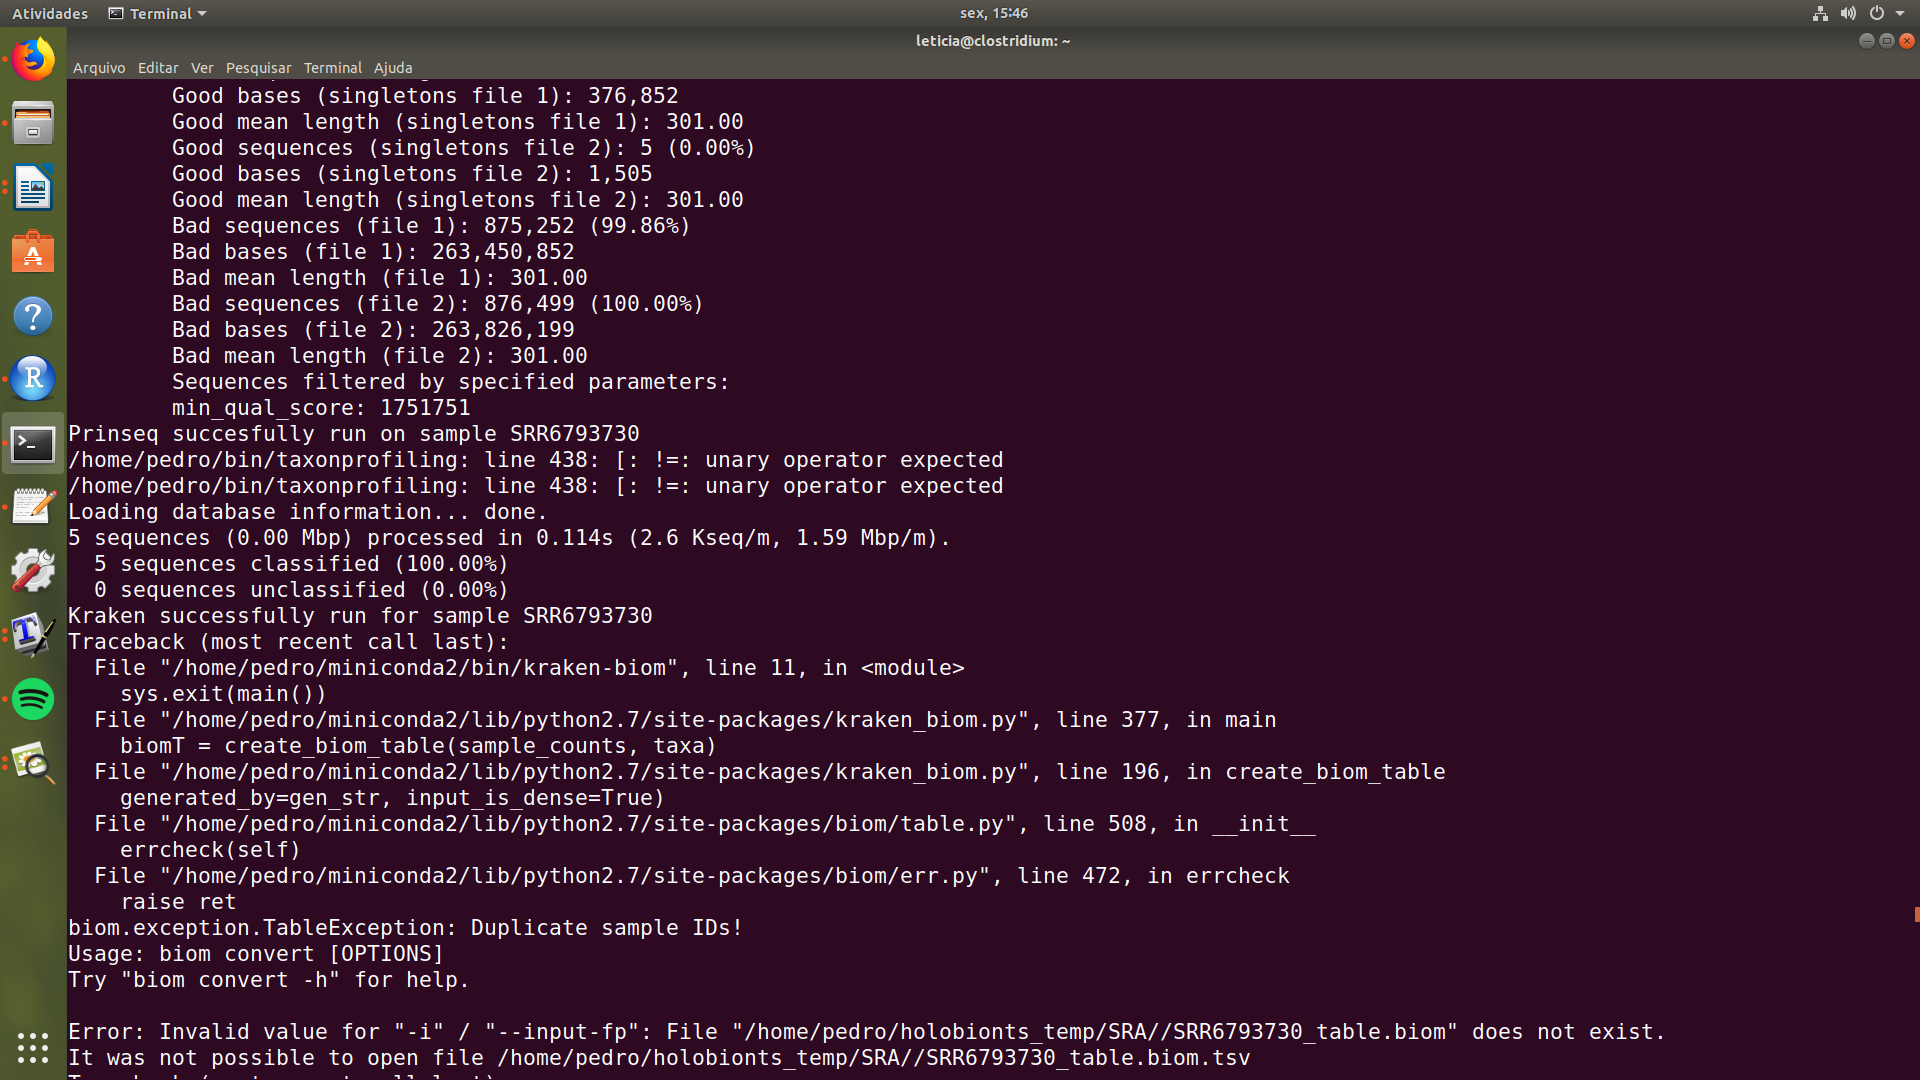
\includegraphics[scale=0.3]{figures/erro_26_10.png}
\caption{Erro com o script taxon profiling se manifestando ao não gerar as matrizes de abundância}
\end{figure}


\newpage
\section{Analises e obtencao de figuras}
Apliquei o tutorial do professor para obtenção de figuras no R para visualização dos resultados. \\
\begin{tcolorbox}[width=6.3in]
- Script: \textit{analisys.R}\\
- Folder: \textit{/home/leticia/Documentos/libs/R}
\end{tcolorbox}

Figuras obtidas:

\begin{figure}[!h]
  \centering 
  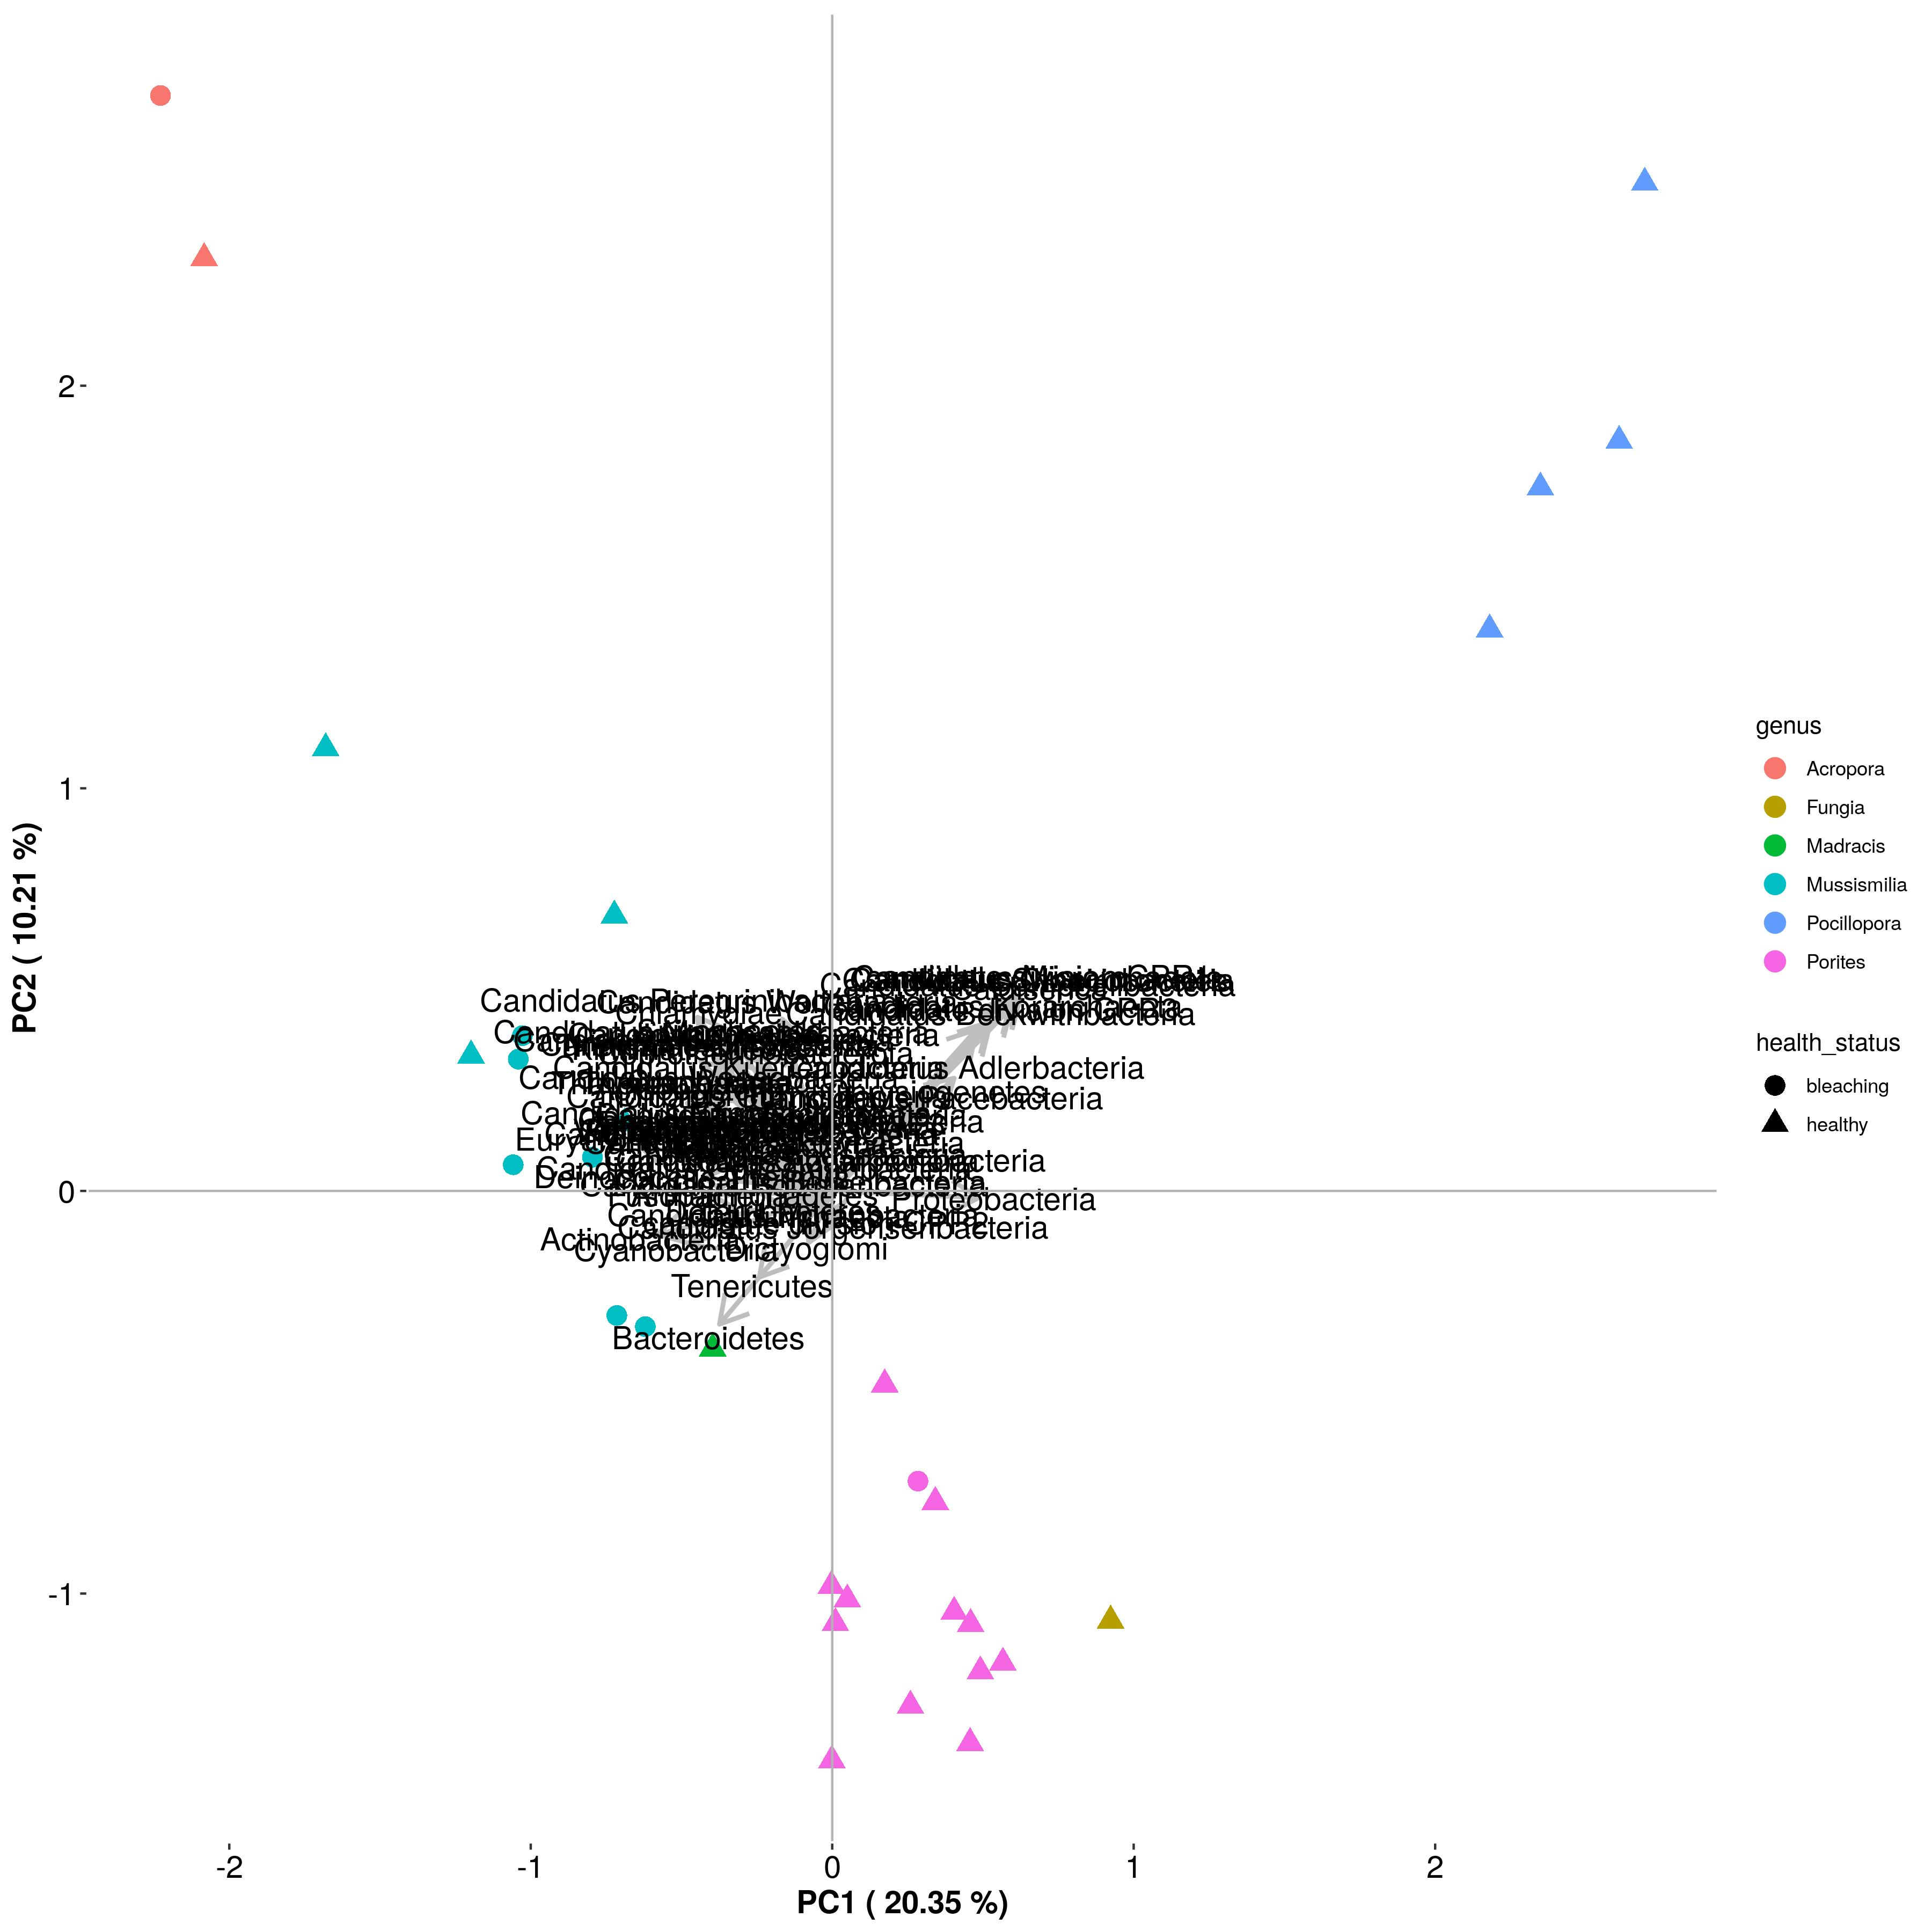
\includegraphics[width=0.9\textwidth]{figures/output_PCA_corais_2018_10_01.jpg}
  \caption{Análise de componentes principais com todos os filos como variaveis}
  \end{figure}

Na analise acima, as variaveis são muitas e ficam muito sobrepostas, fazendo com que haja grande poluicao visual. O professor recomendou em marco a utilizar uma analise de Random Forest, para que as variaveis mais importantes para os metagenomas que trabalho sejam ranqueadas. O random forest é um algoritmo de machine learning que, a partir das duas categorias de saúde (categorias de supervisao), elencará as variáveis mais importantes para classificar as amostras nesses dois estados. o random forest abaixo é supervisionado por estado de saúde \\

\begin{figure}[!h]
  \centering 
  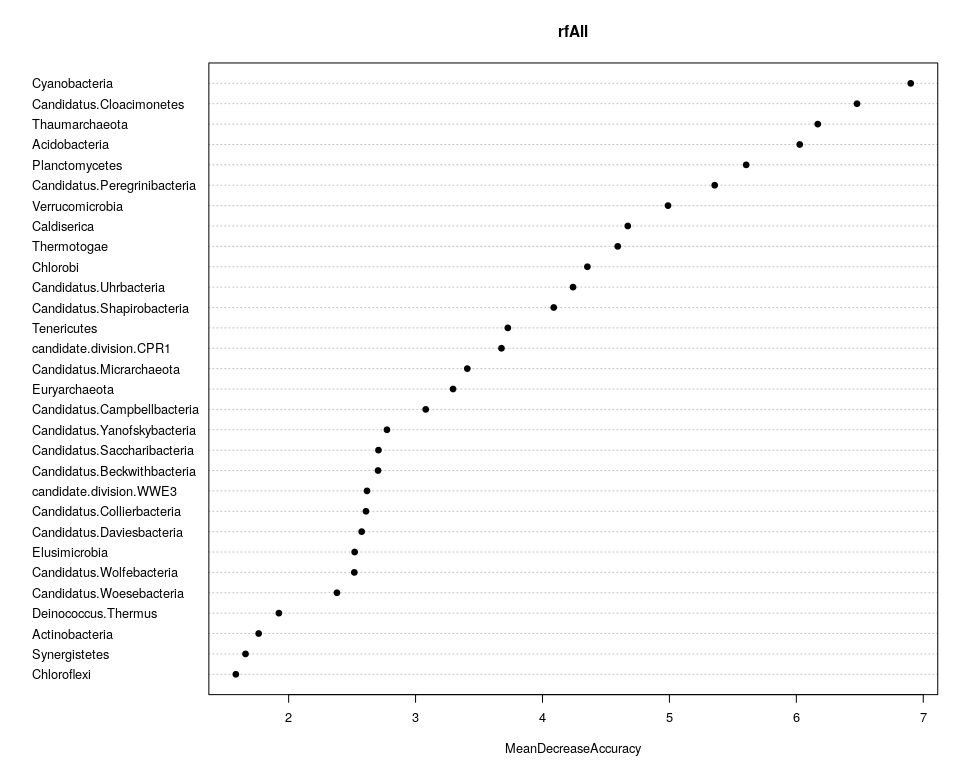
\includegraphics[width=0.7\textwidth]{figures/randomforest_taxonomic_corais_2018_10_01.jpeg}
  \caption{Random Forest ranqueando filos}
  \end{figure}

Eu utilizei os 20 primeiros filos ranqueados para fazer o PCA. Segue esse PCA abaixo:

\begin{figure}[!h]
  \centering 
  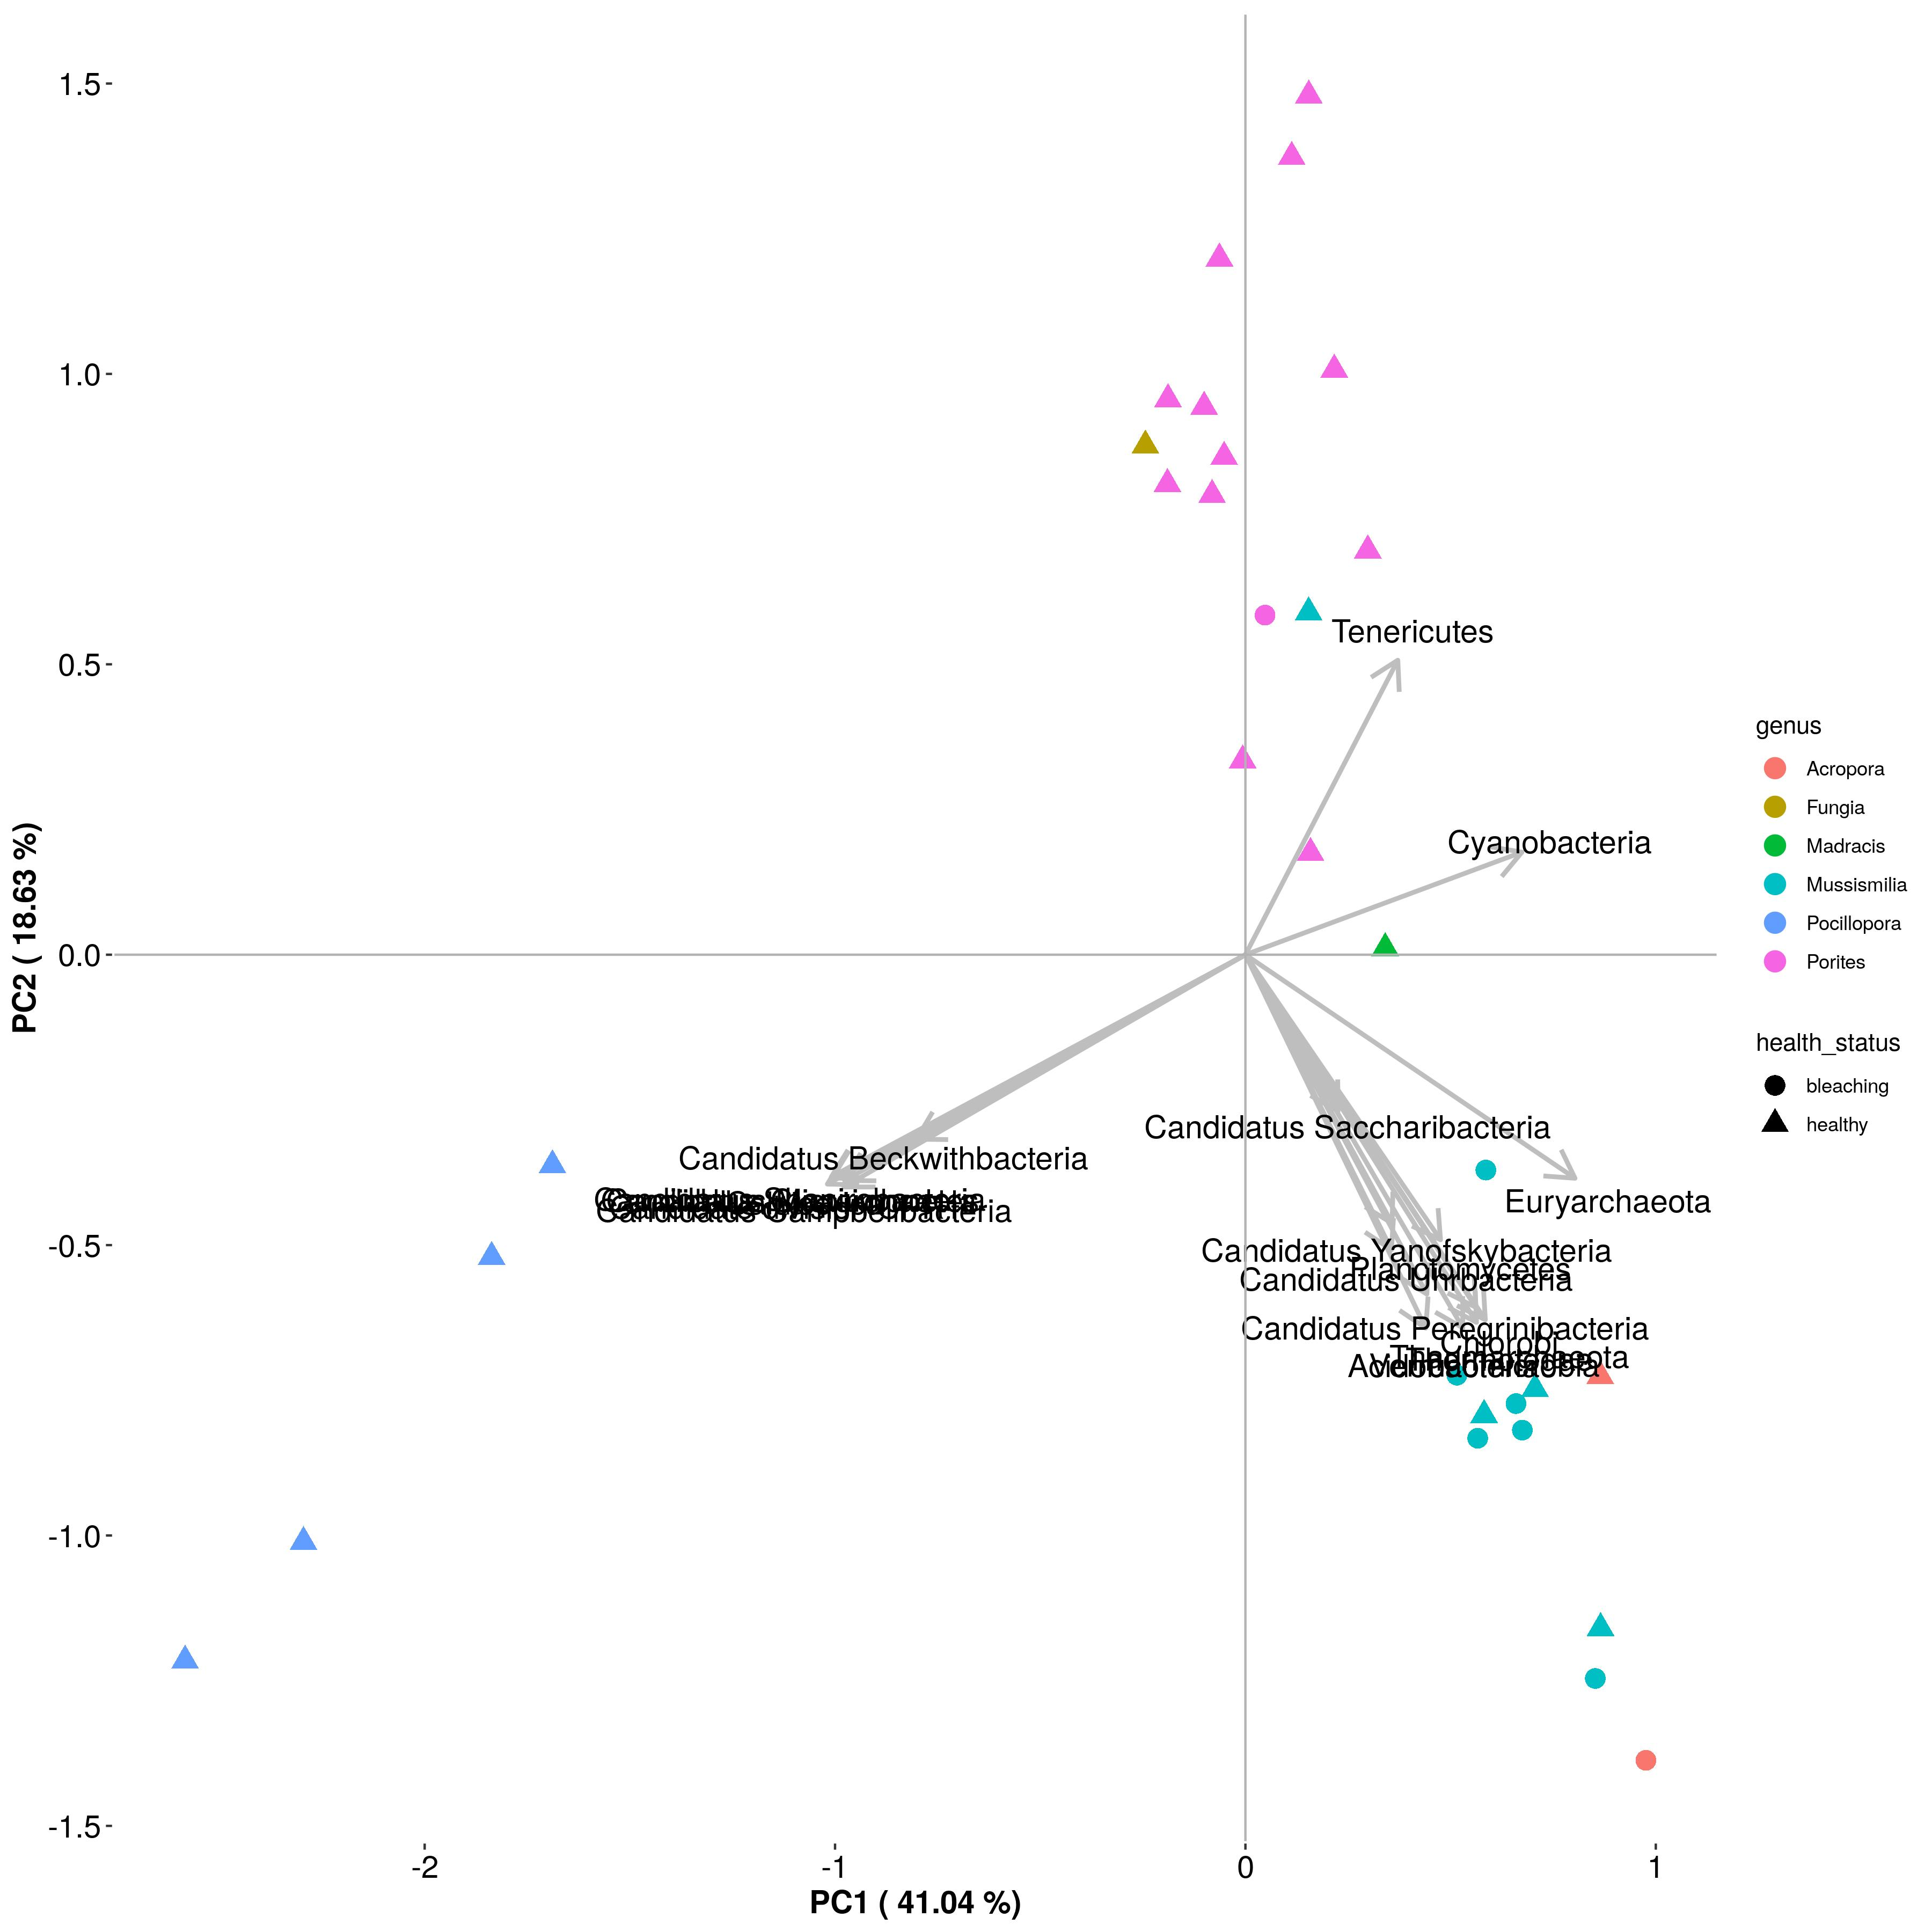
\includegraphics[width=0.6\textwidth]{figures/output_rf_20_PCA_corais_2018_10_01.jpg}
  \caption{PCA com 20 filos utilizados no PCA}
  \end{figure}
\newpage
Uma tendencia se manteve: foi a separação das amostras por genero.  Mas a poluicao visual ainda continuou, por isso fiz um random forest com os 15 primeiros filos indicados pelo random forest. Segue abaixo: 
\begin{figure}[!h]
  \centering 
  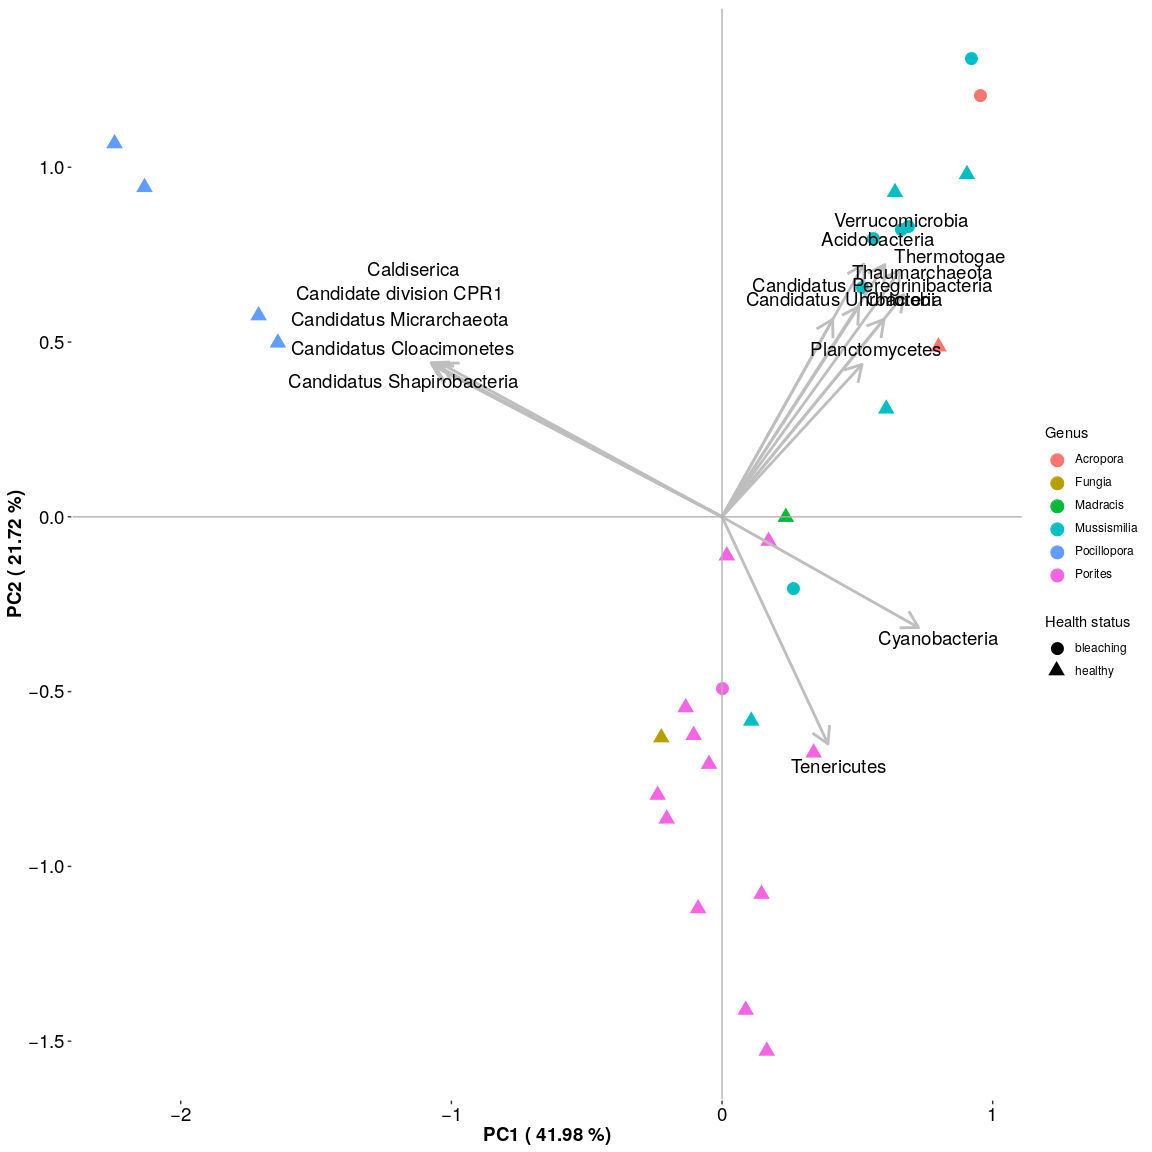
\includegraphics[width=0.9\textwidth]{figures/output_rf_15_PCA_corais_2018_10_01_edited_3.png}
  \caption{PCA com 15 filos como variaveis}
  \end{figure}

Algumas tendencias tambem se mantiveram e a explicação dos eixos melhorou levemente. As amostras agrupadas no quadrante direito superior são mais diferentes das que estão no quadrante esquerdo do que das que estão no quadrante inferior direito. Na reuniao feita no dia 03/10/2018, o Amaro, o professor e Miguel me sinalizaram que existe uma separacao forte entre generos, indicando que os grupos candidatos podem ser genero - específicos. Surgiu a sugestão de leitura de textos em core microbiome e especificidade de filos entre generos e o professor sugeriu fazer um random forest nao supervisionado que segue abaixo. O professor Garcia no congresso sugeriu utilizar os auto valores do PCA para ver quais podem ser mais relevantes (?).

\begin{figure}[H]
\centering
  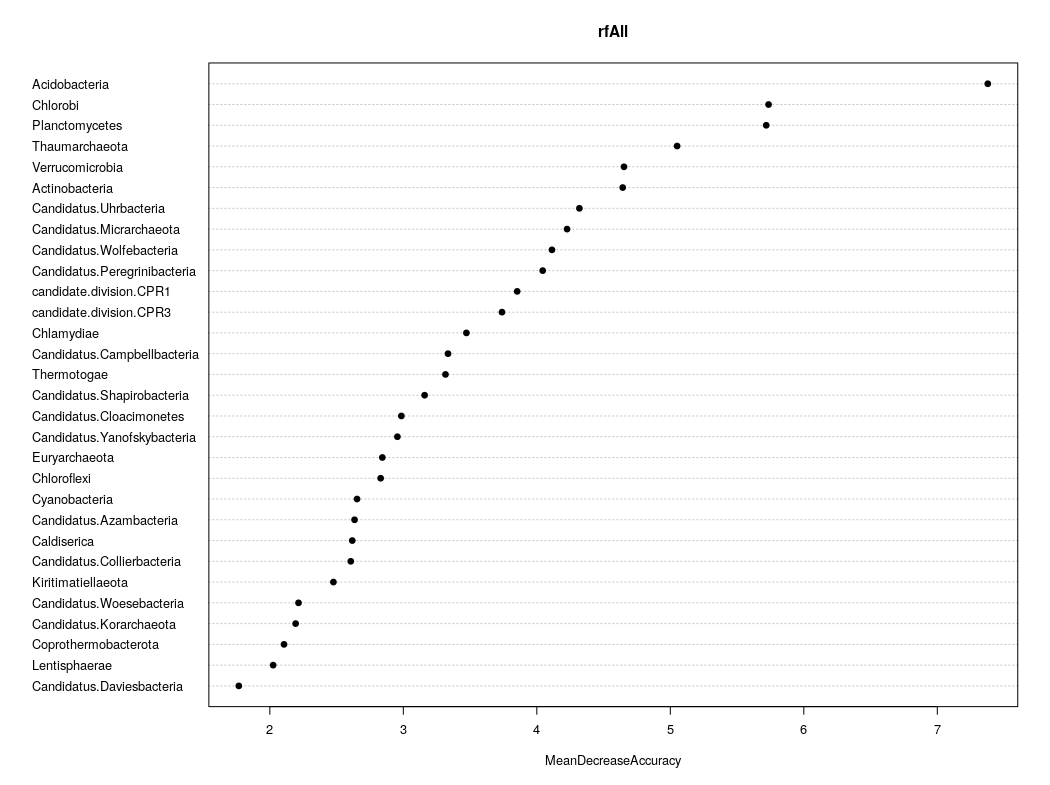
\includegraphics[scale=0.5]{figures/randomforest_nao_supervisionado_corais_leticia_2018_10_18.jpeg}
  \caption{Random Forest nao supervisionado}
  \end{figure}

Fiz um pca (libs/R/analisys.R) a partir dos primeiros 15 filos indicados no Random Forest  nao supervisionado acima. Segue abaixo:

\begin{figure}[H]
  \centering 
  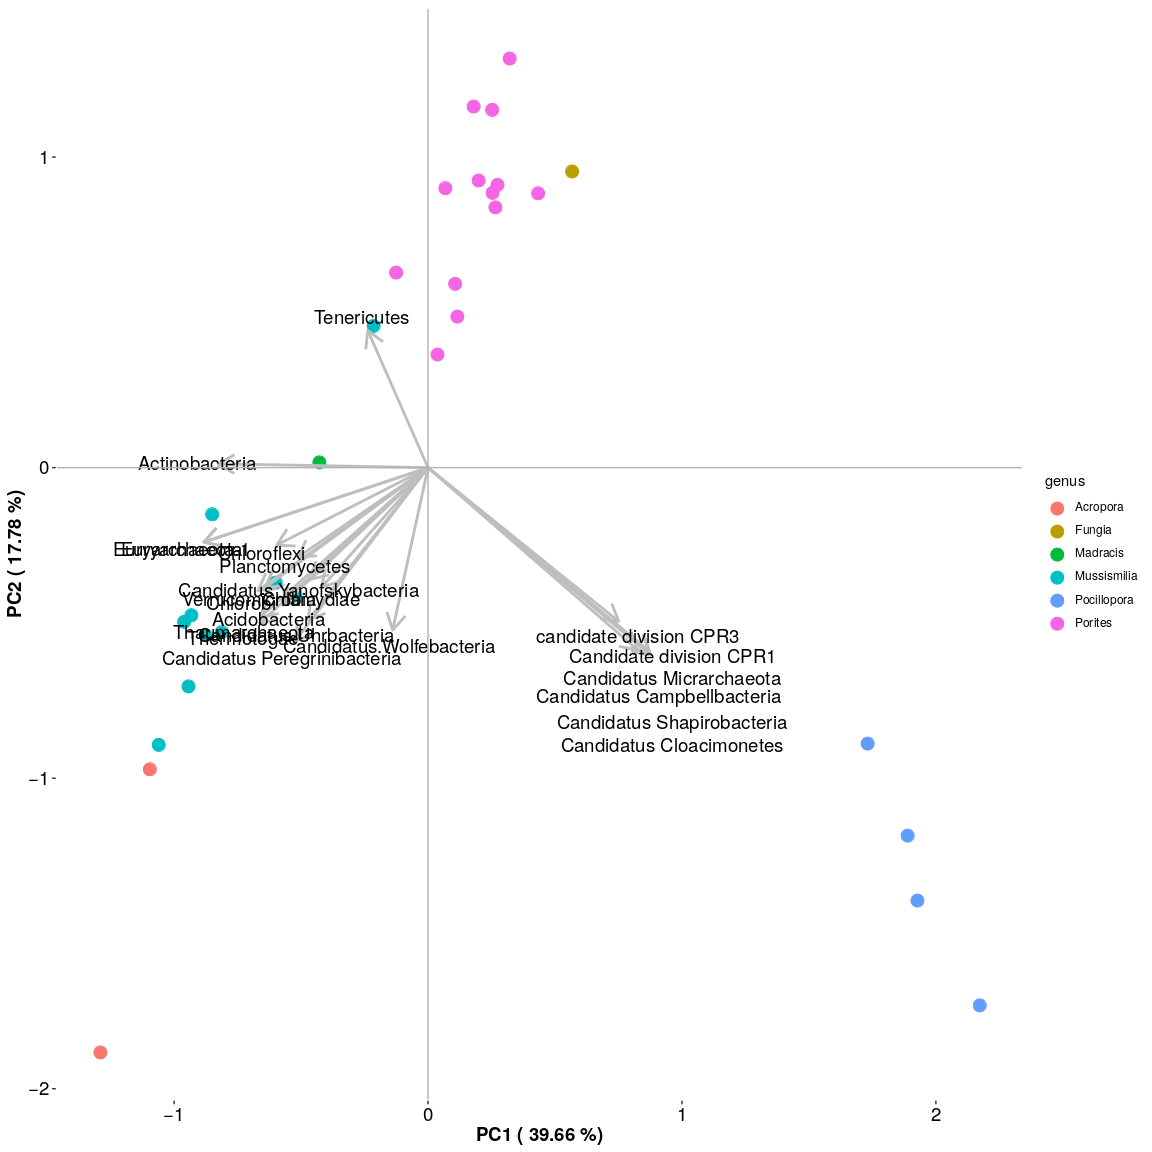
\includegraphics[width=0.6\textwidth]{figures/rf_nao_supervisionado_pca_corais_20_filos_15_10_2018_edited.png}
  \caption{PCA a partir dos 20 filos primeiros filos que aparecem acima no random forest}
  \end{figure}

\begin{figure}[H]
  \centering 
  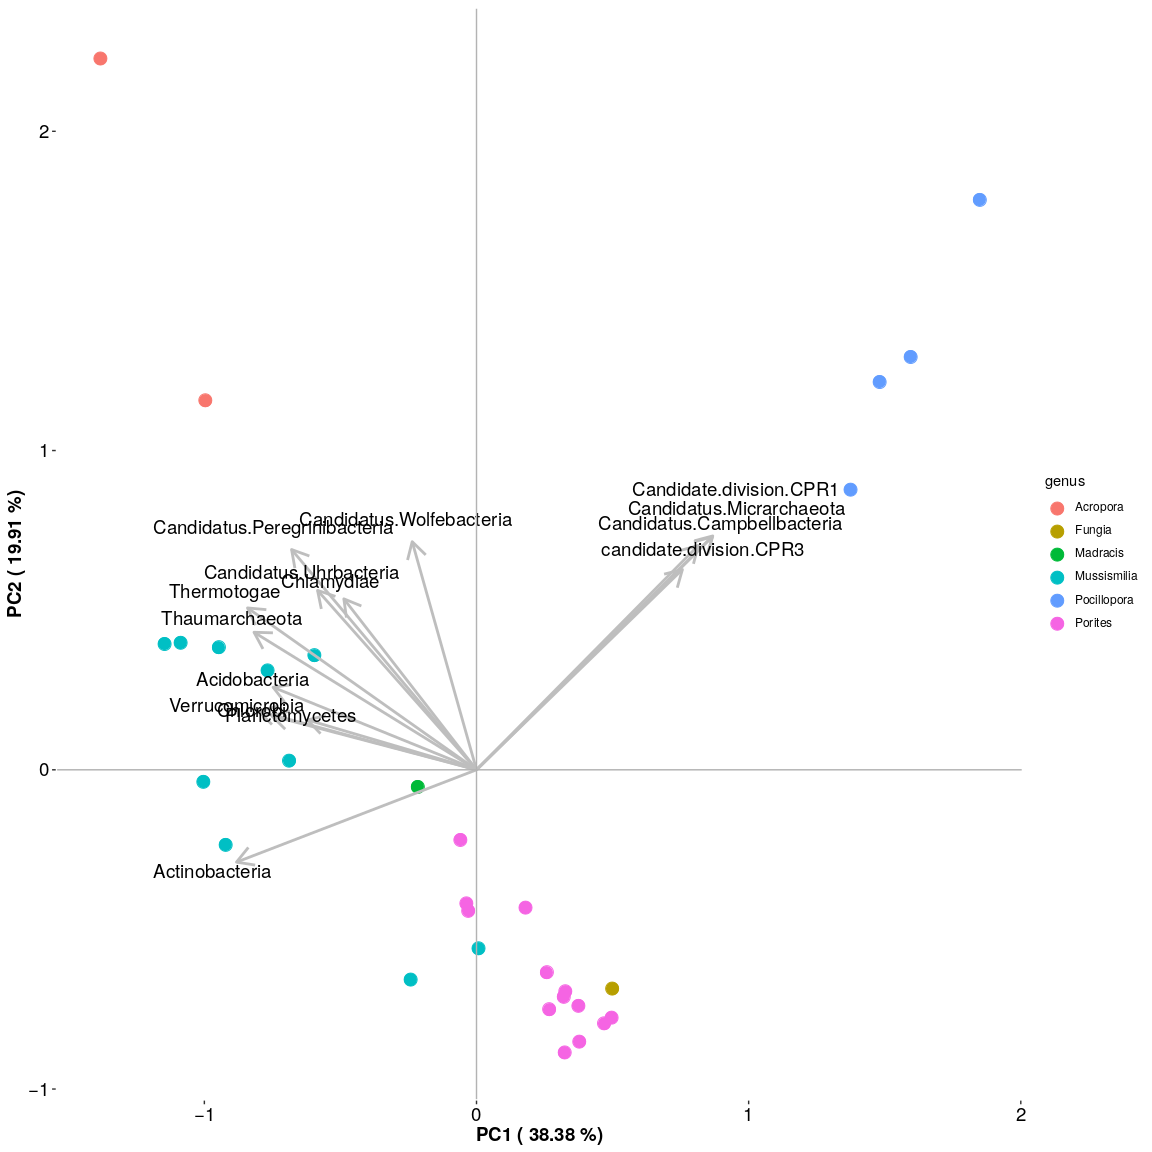
\includegraphics[width=0.9\textwidth]{figures/rf_nao_supervisionado_pca_corais_15_filos_15_10_2018_edited.png}
  \caption{PCA a partir dos 15 filos primeiros filos que aparecem acima no random forest nao supervisionado}
  \end{figure}

\newpage
\section{Obtencao de figuras com o segundo profiling feito com a ajuda do Rilquer - 23/10/2018}  
As figuras a seguir foram feitas com dados de abundancia gerados com a ajuda do Rilquer. As primeiras serao com abundancia dos metagenomas do MG-RAST.

\begin{figure}[!h]
  \centering
  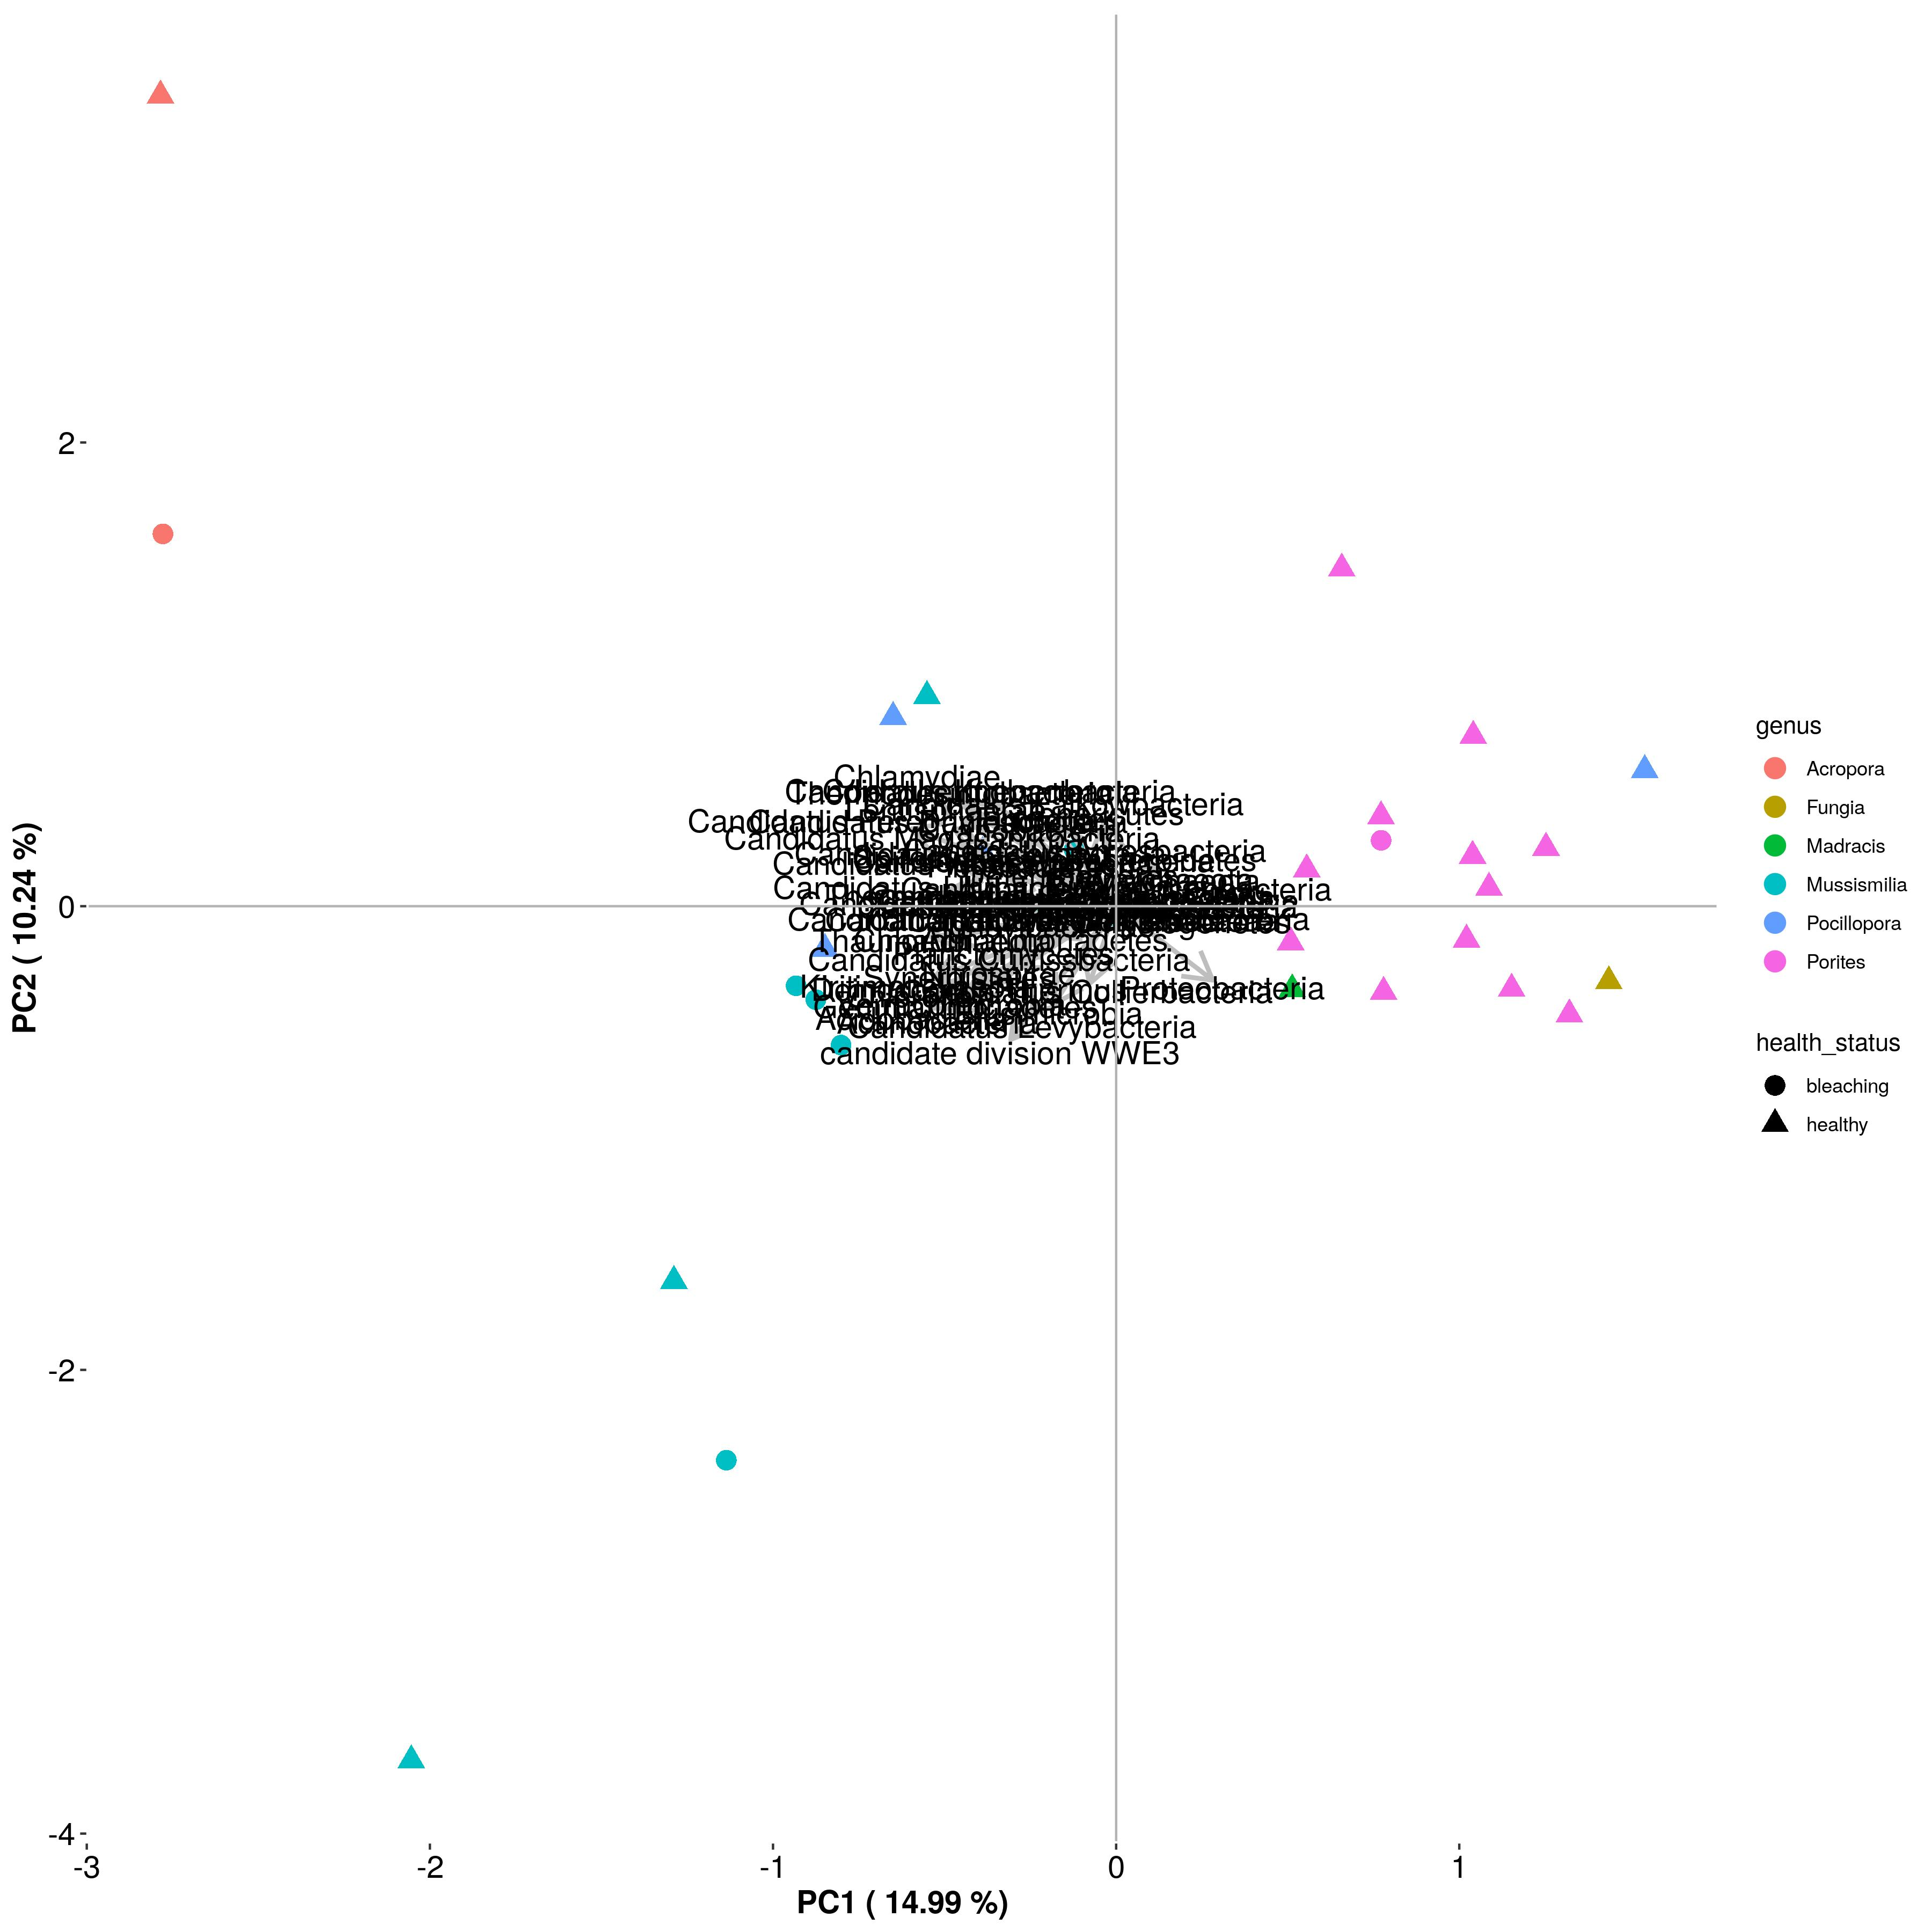
\includegraphics[scale=0.5]{figures/output_PCA_corais_mg_rast_2018_10_23.jpg}
  \caption{PCA das amostras de metagenomas do mg rast com todos os filos}
\end{figure}

\begin{figure}[H]
\centering
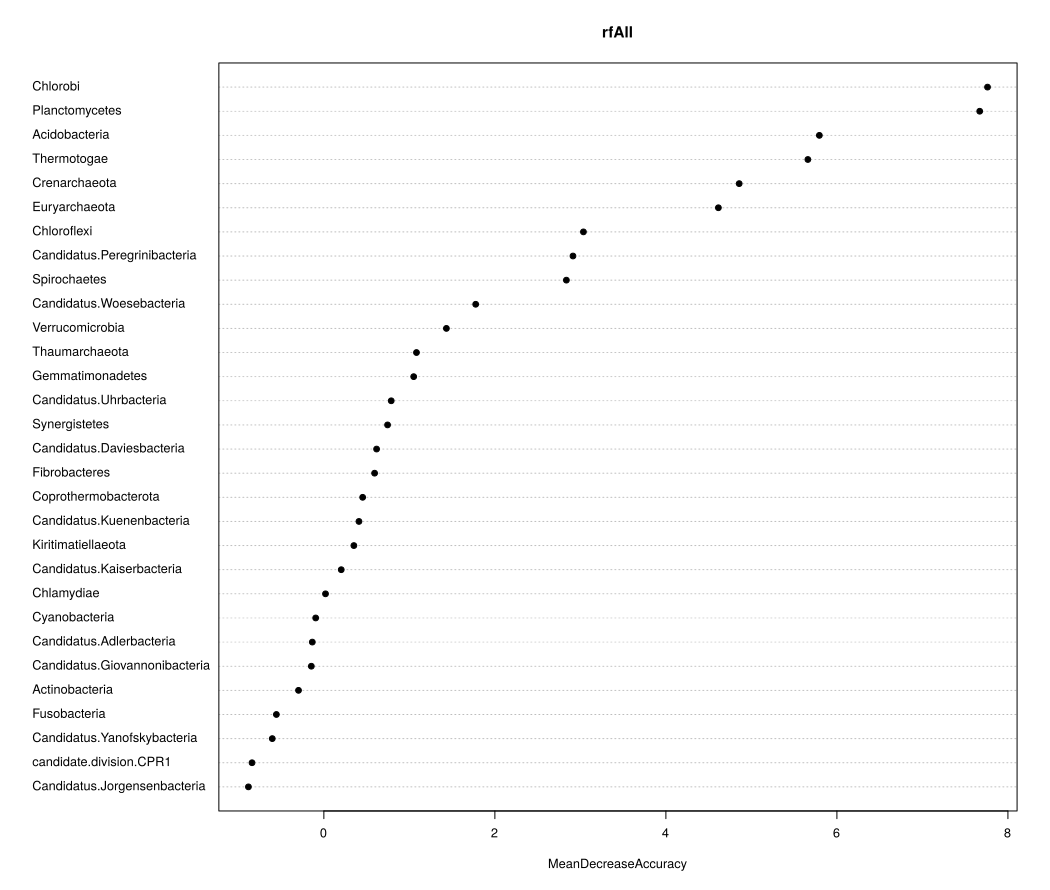
\includegraphics[scale=0.5]{figures/randomforest_nao_supervisionado_corais_mg_rast_leticia_2018_10_23.png}
\caption{Random Forest não supervisionado dos metagenomas de corais do MG-RAST analisadas com a base definitiva}
\end{figure}

\begin{figure}[H]
\centering
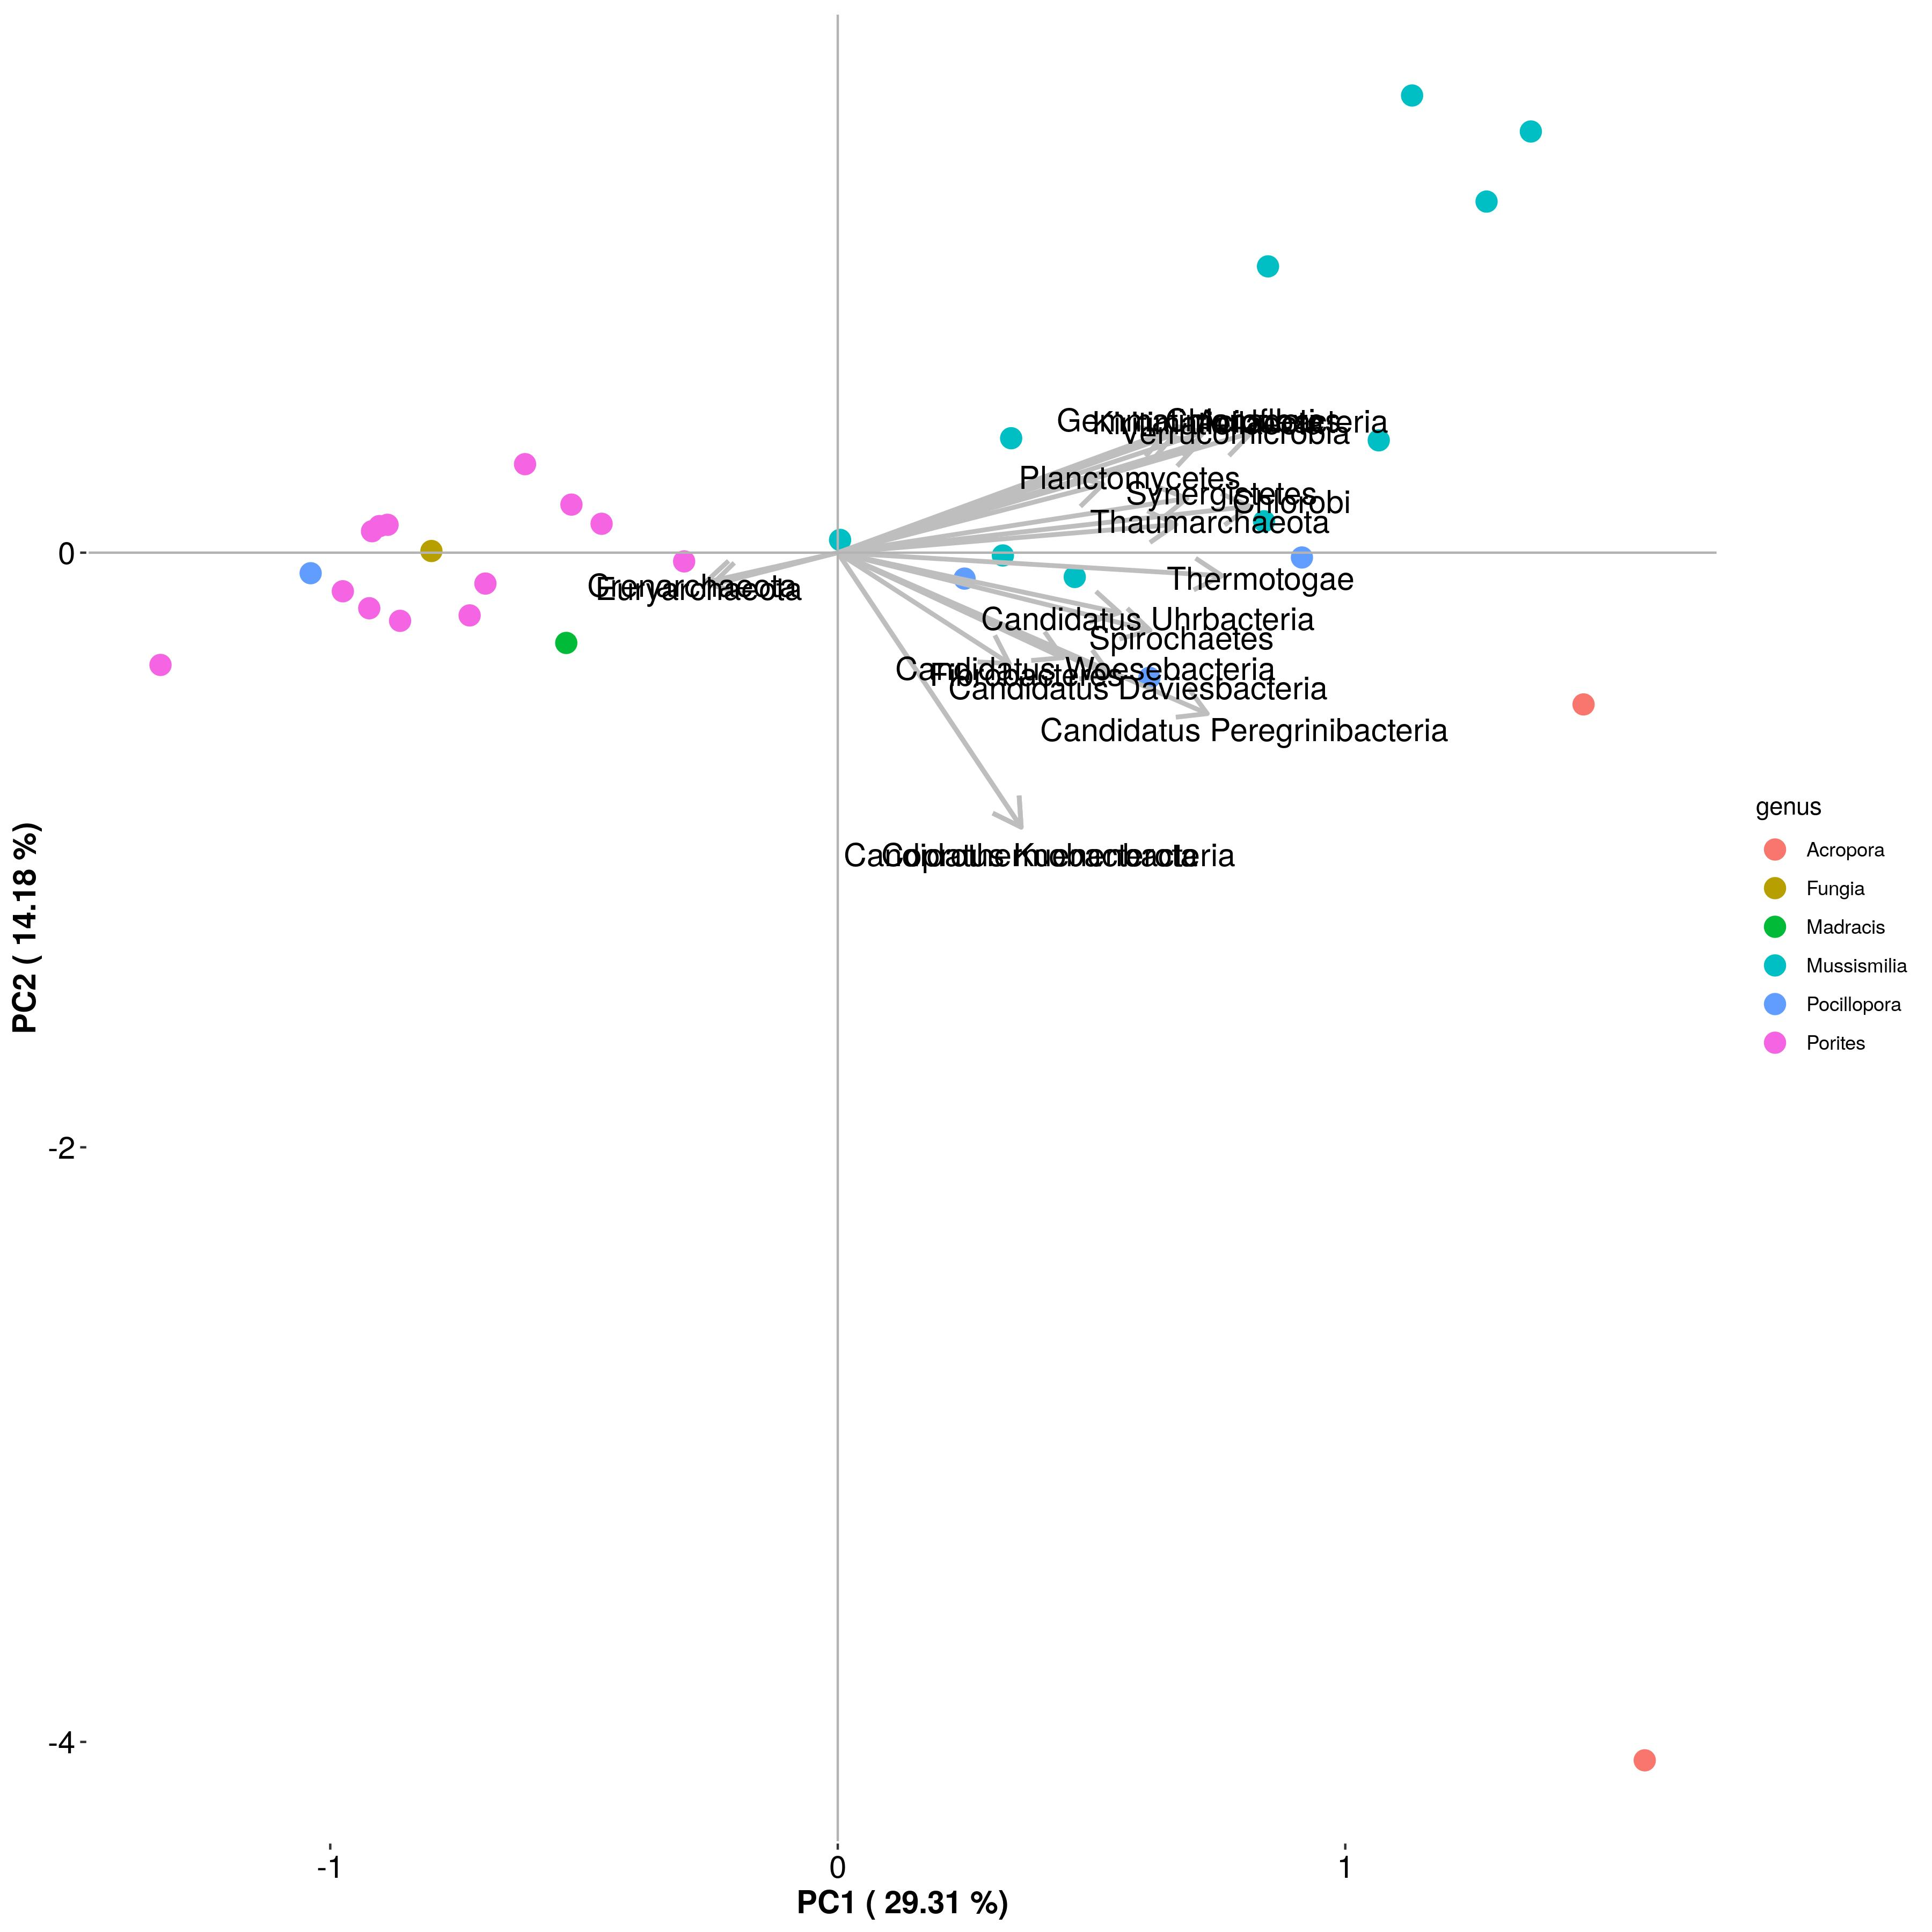
\includegraphics[scale=0.4]{figures/pca_corais_rf_nao_supervisionado_20_filos_23_10_2018.jpg}
\caption{PCA GERADO COM OS PRIMEIROS 20 FILOS DO RANDOM FOREST NAO SUPERVISIONADO ACIMA}
\end{figure}

\begin{figure}[H]
\centering
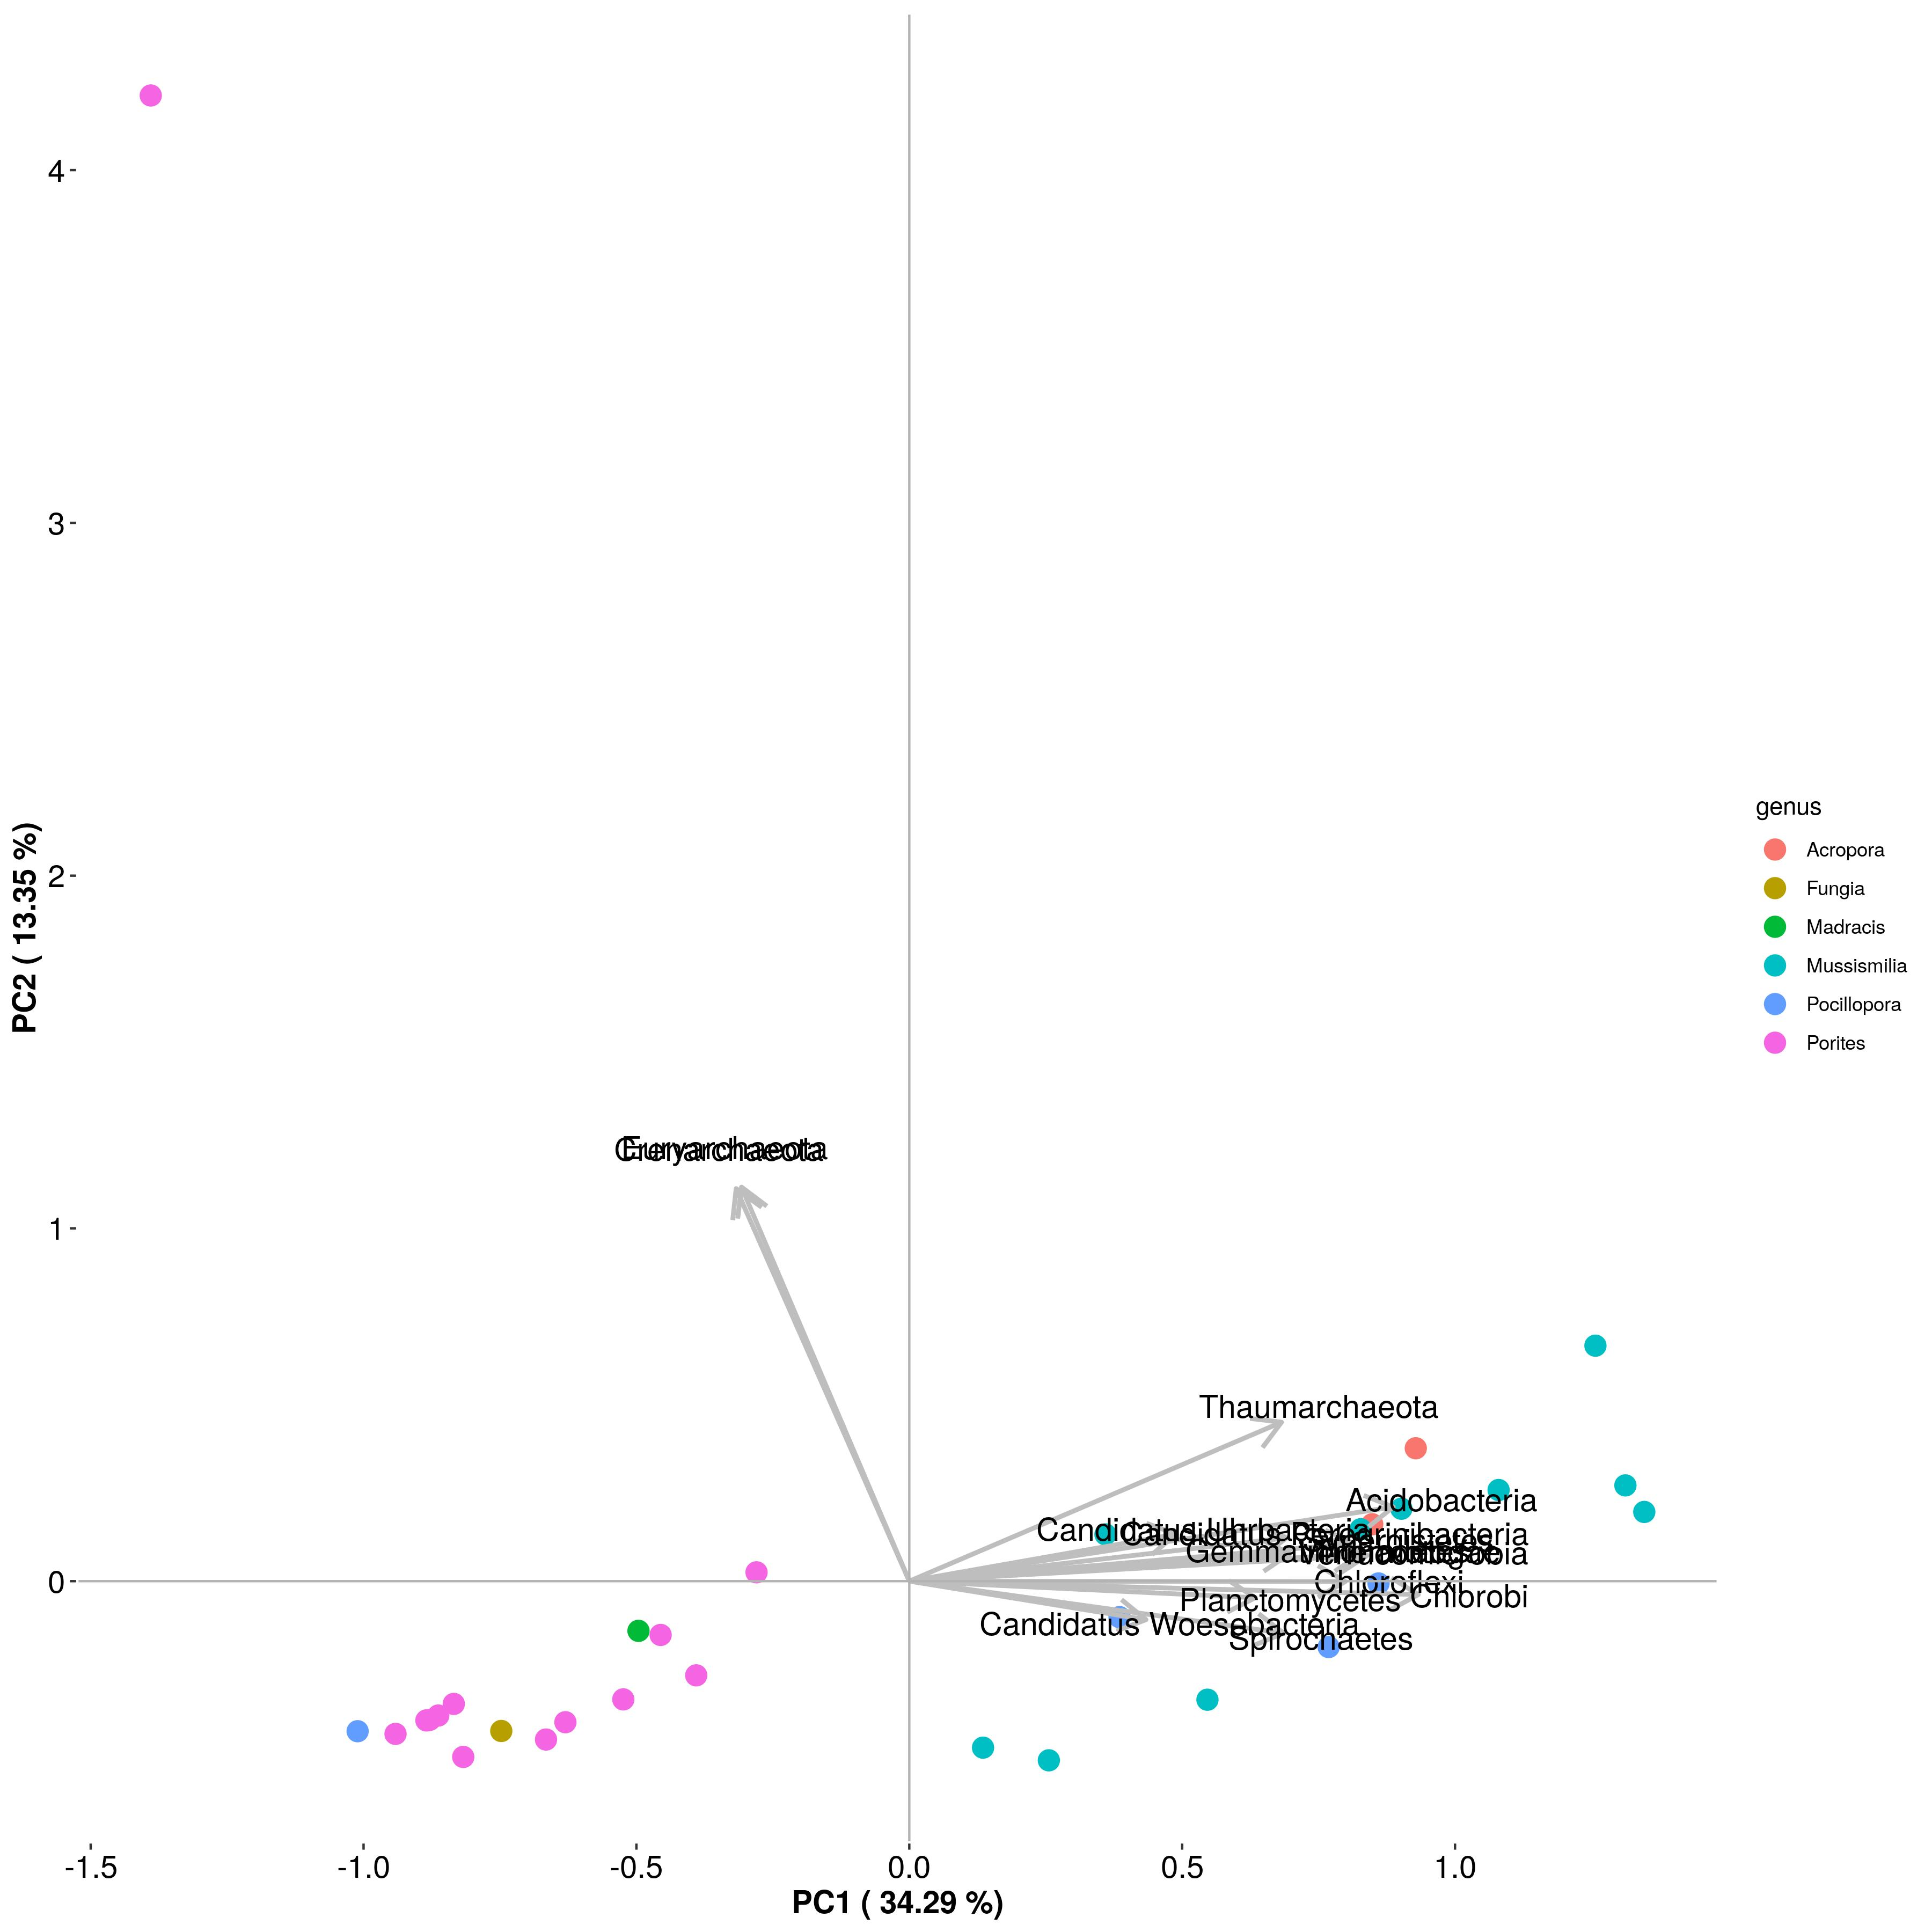
\includegraphics[scale=0.4]{figures/pca_corais_rf_nao_supervisionado_15_filos_23_10_2018.jpg}
\caption{PCA GERADO COM OS PRIMEIROS 15 FILOS DO RANDOM FOREST NAO SUPERVISIONADO}
\end{figure}

\begin{figure}[H]
\centering
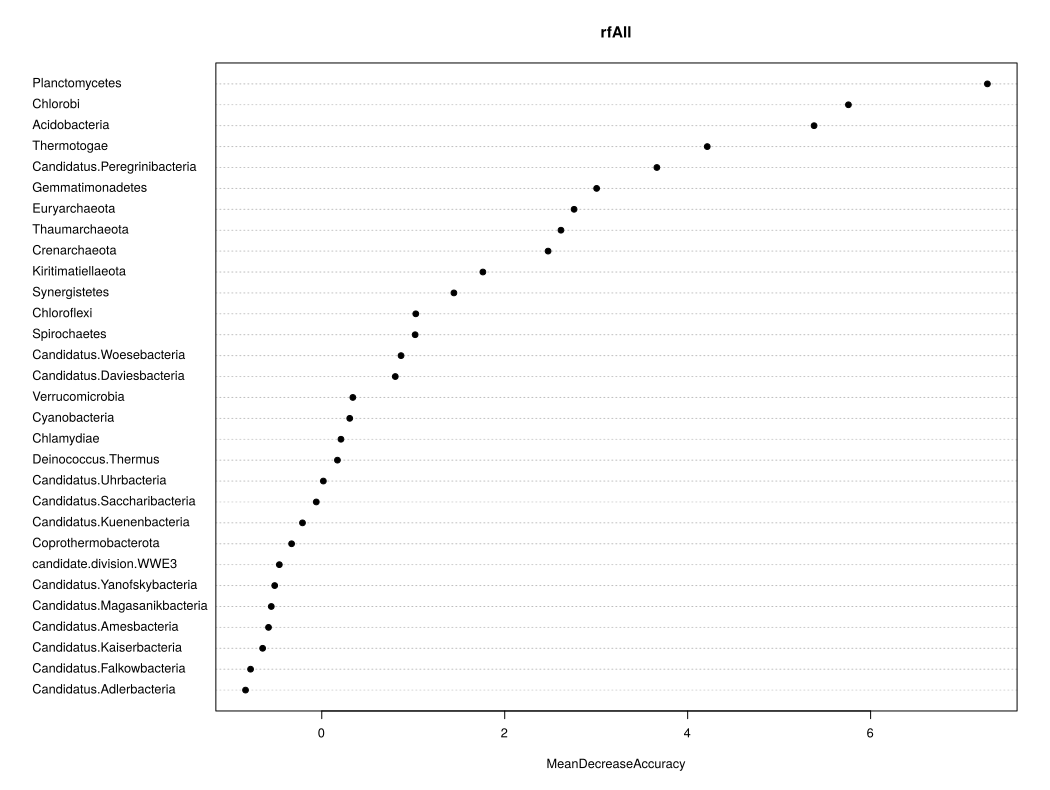
\includegraphics[scale=0.4]{figures/randomforest_supervisionado_genero_corais_leticia_2018_10_23.png}
\caption{RANDOM FOREST SUPERVISIONADO POR GENERO DOS METAGENOMAS DE CORAIS DO MG RAST ANALISADOS COM A BASE DEFINITIVA}
\end{figure}

\begin{figure}[H]
\centering
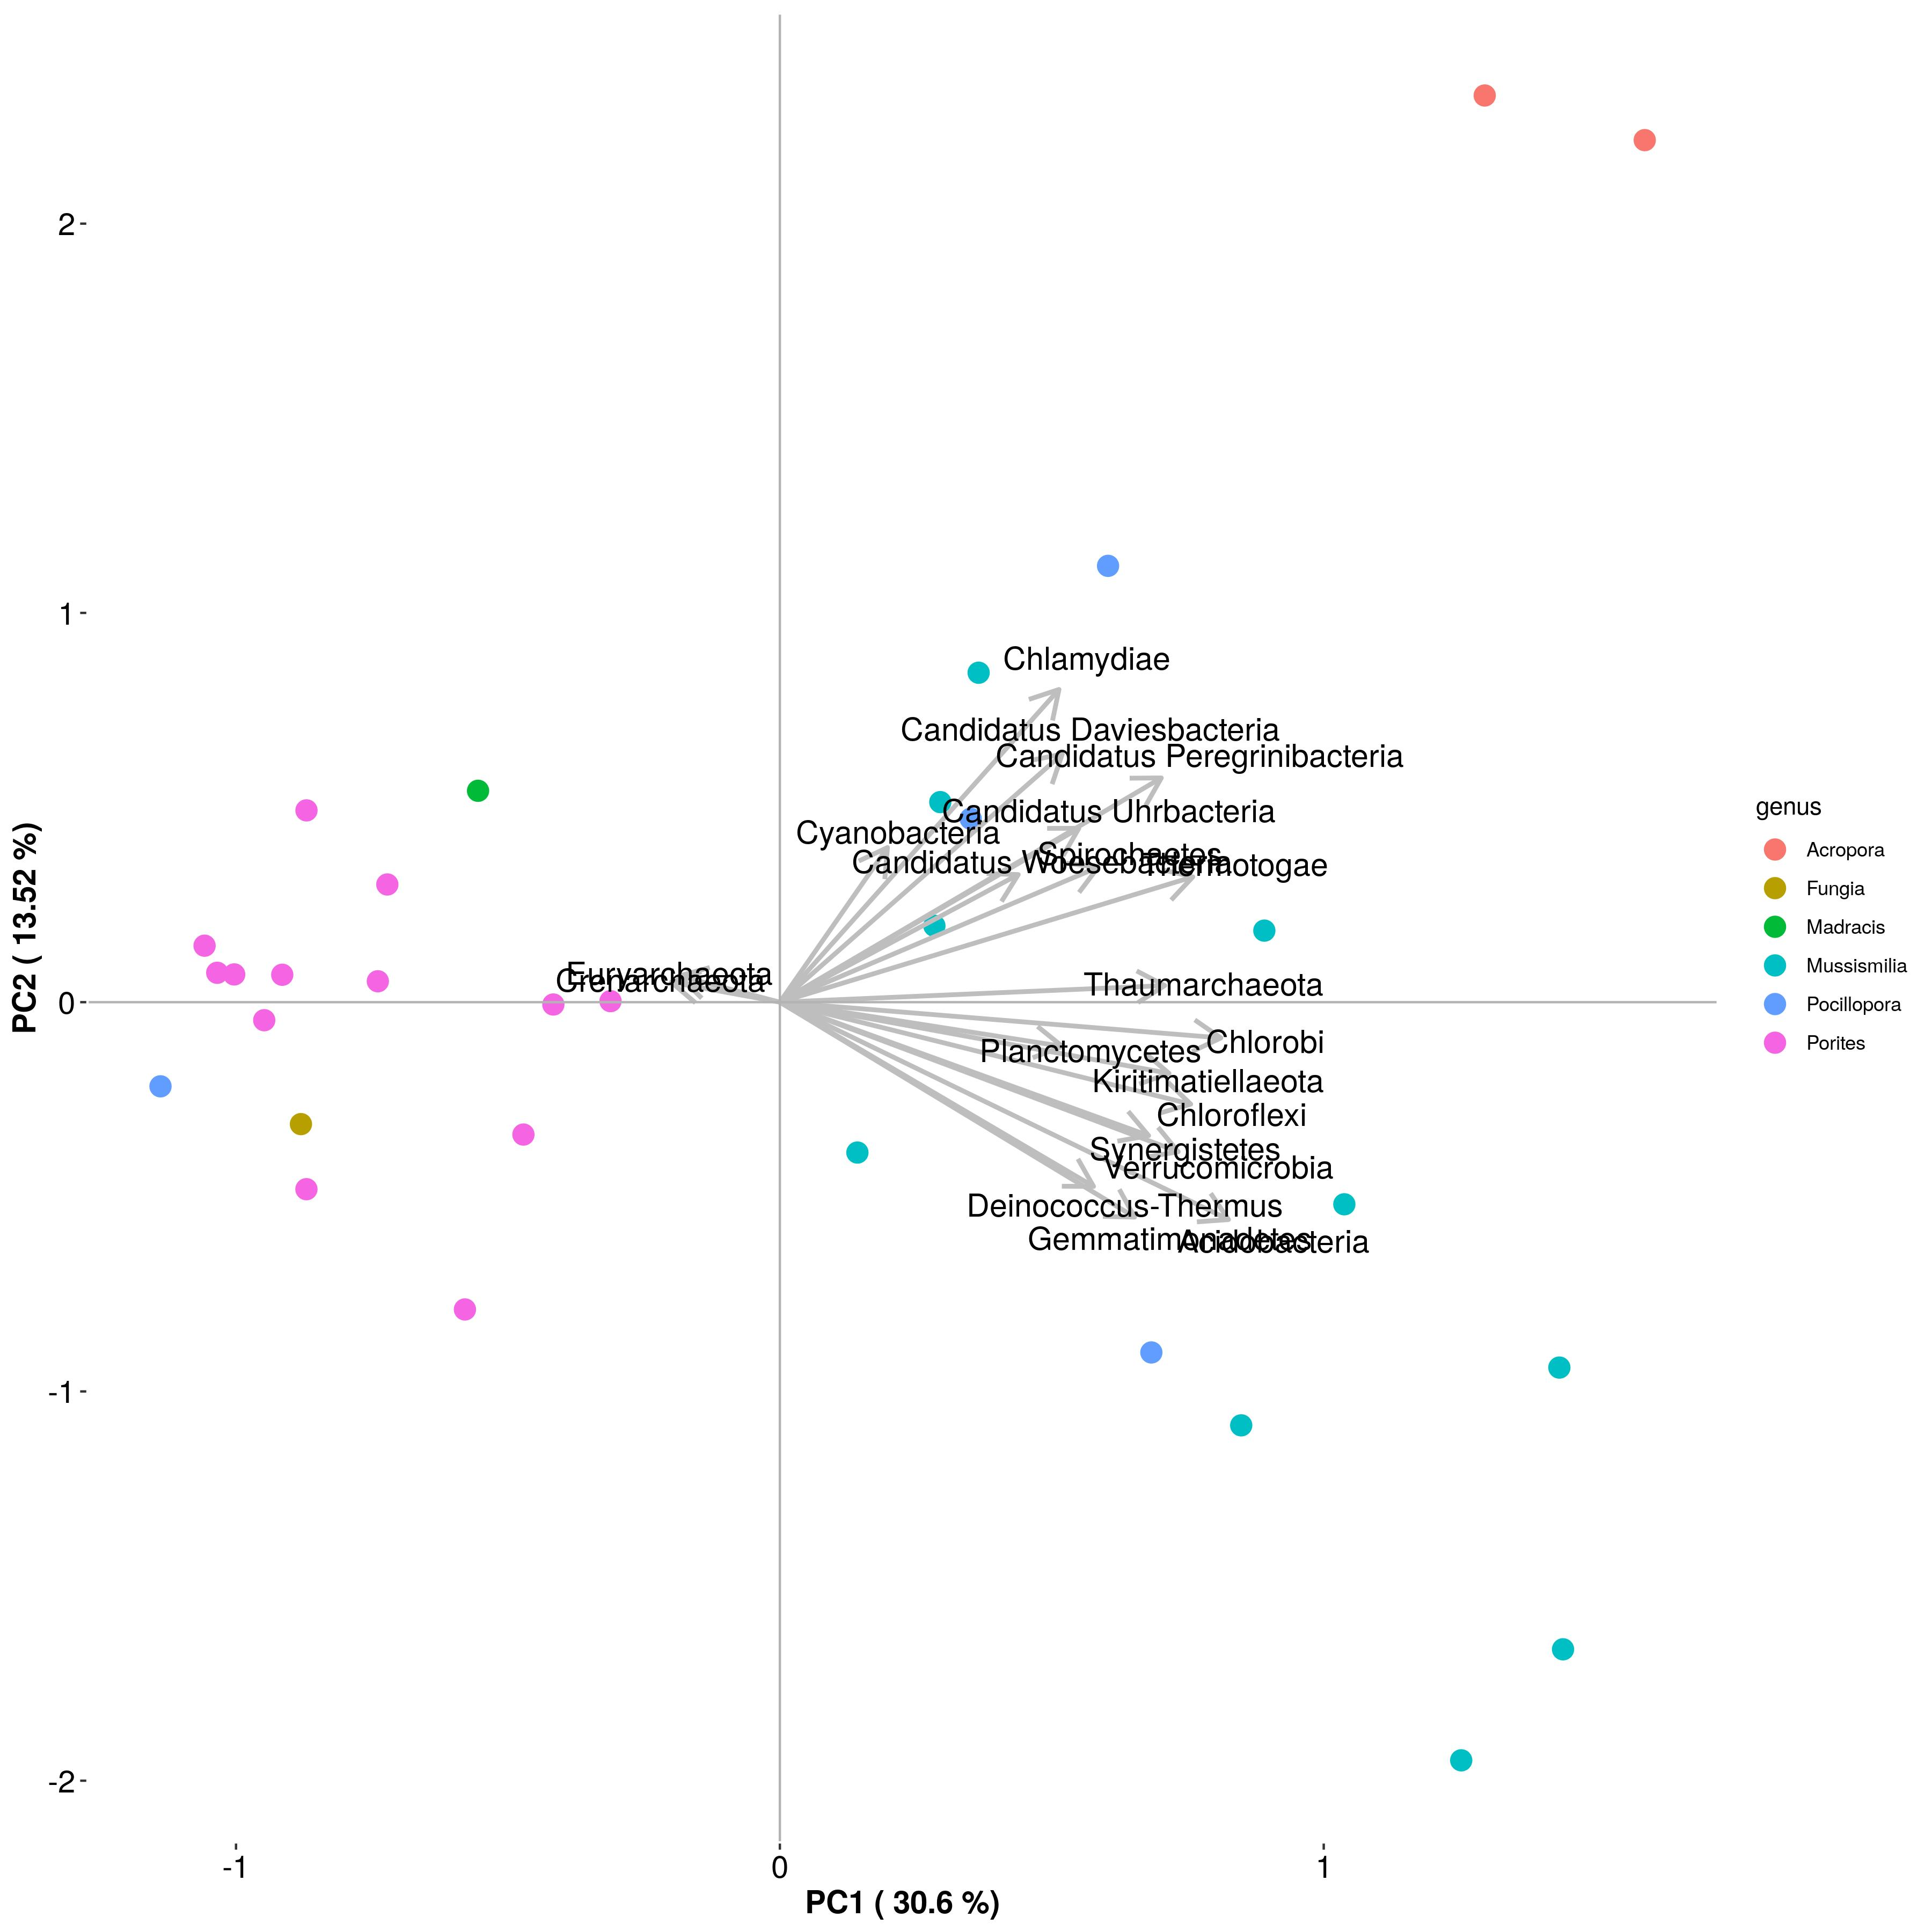
\includegraphics[scale=0.4]{figures/pca_corais_mg_rast_rf_supervisionado_genus_20_filos_23_10_2018.jpg}
\caption{PCA GERADO COM OS PRIMEIROS 20 FILOS DO RANDOM FOREST SUPERVISIONADO POR GENERO}
\end{figure}

\begin{figure}[H]
\centering
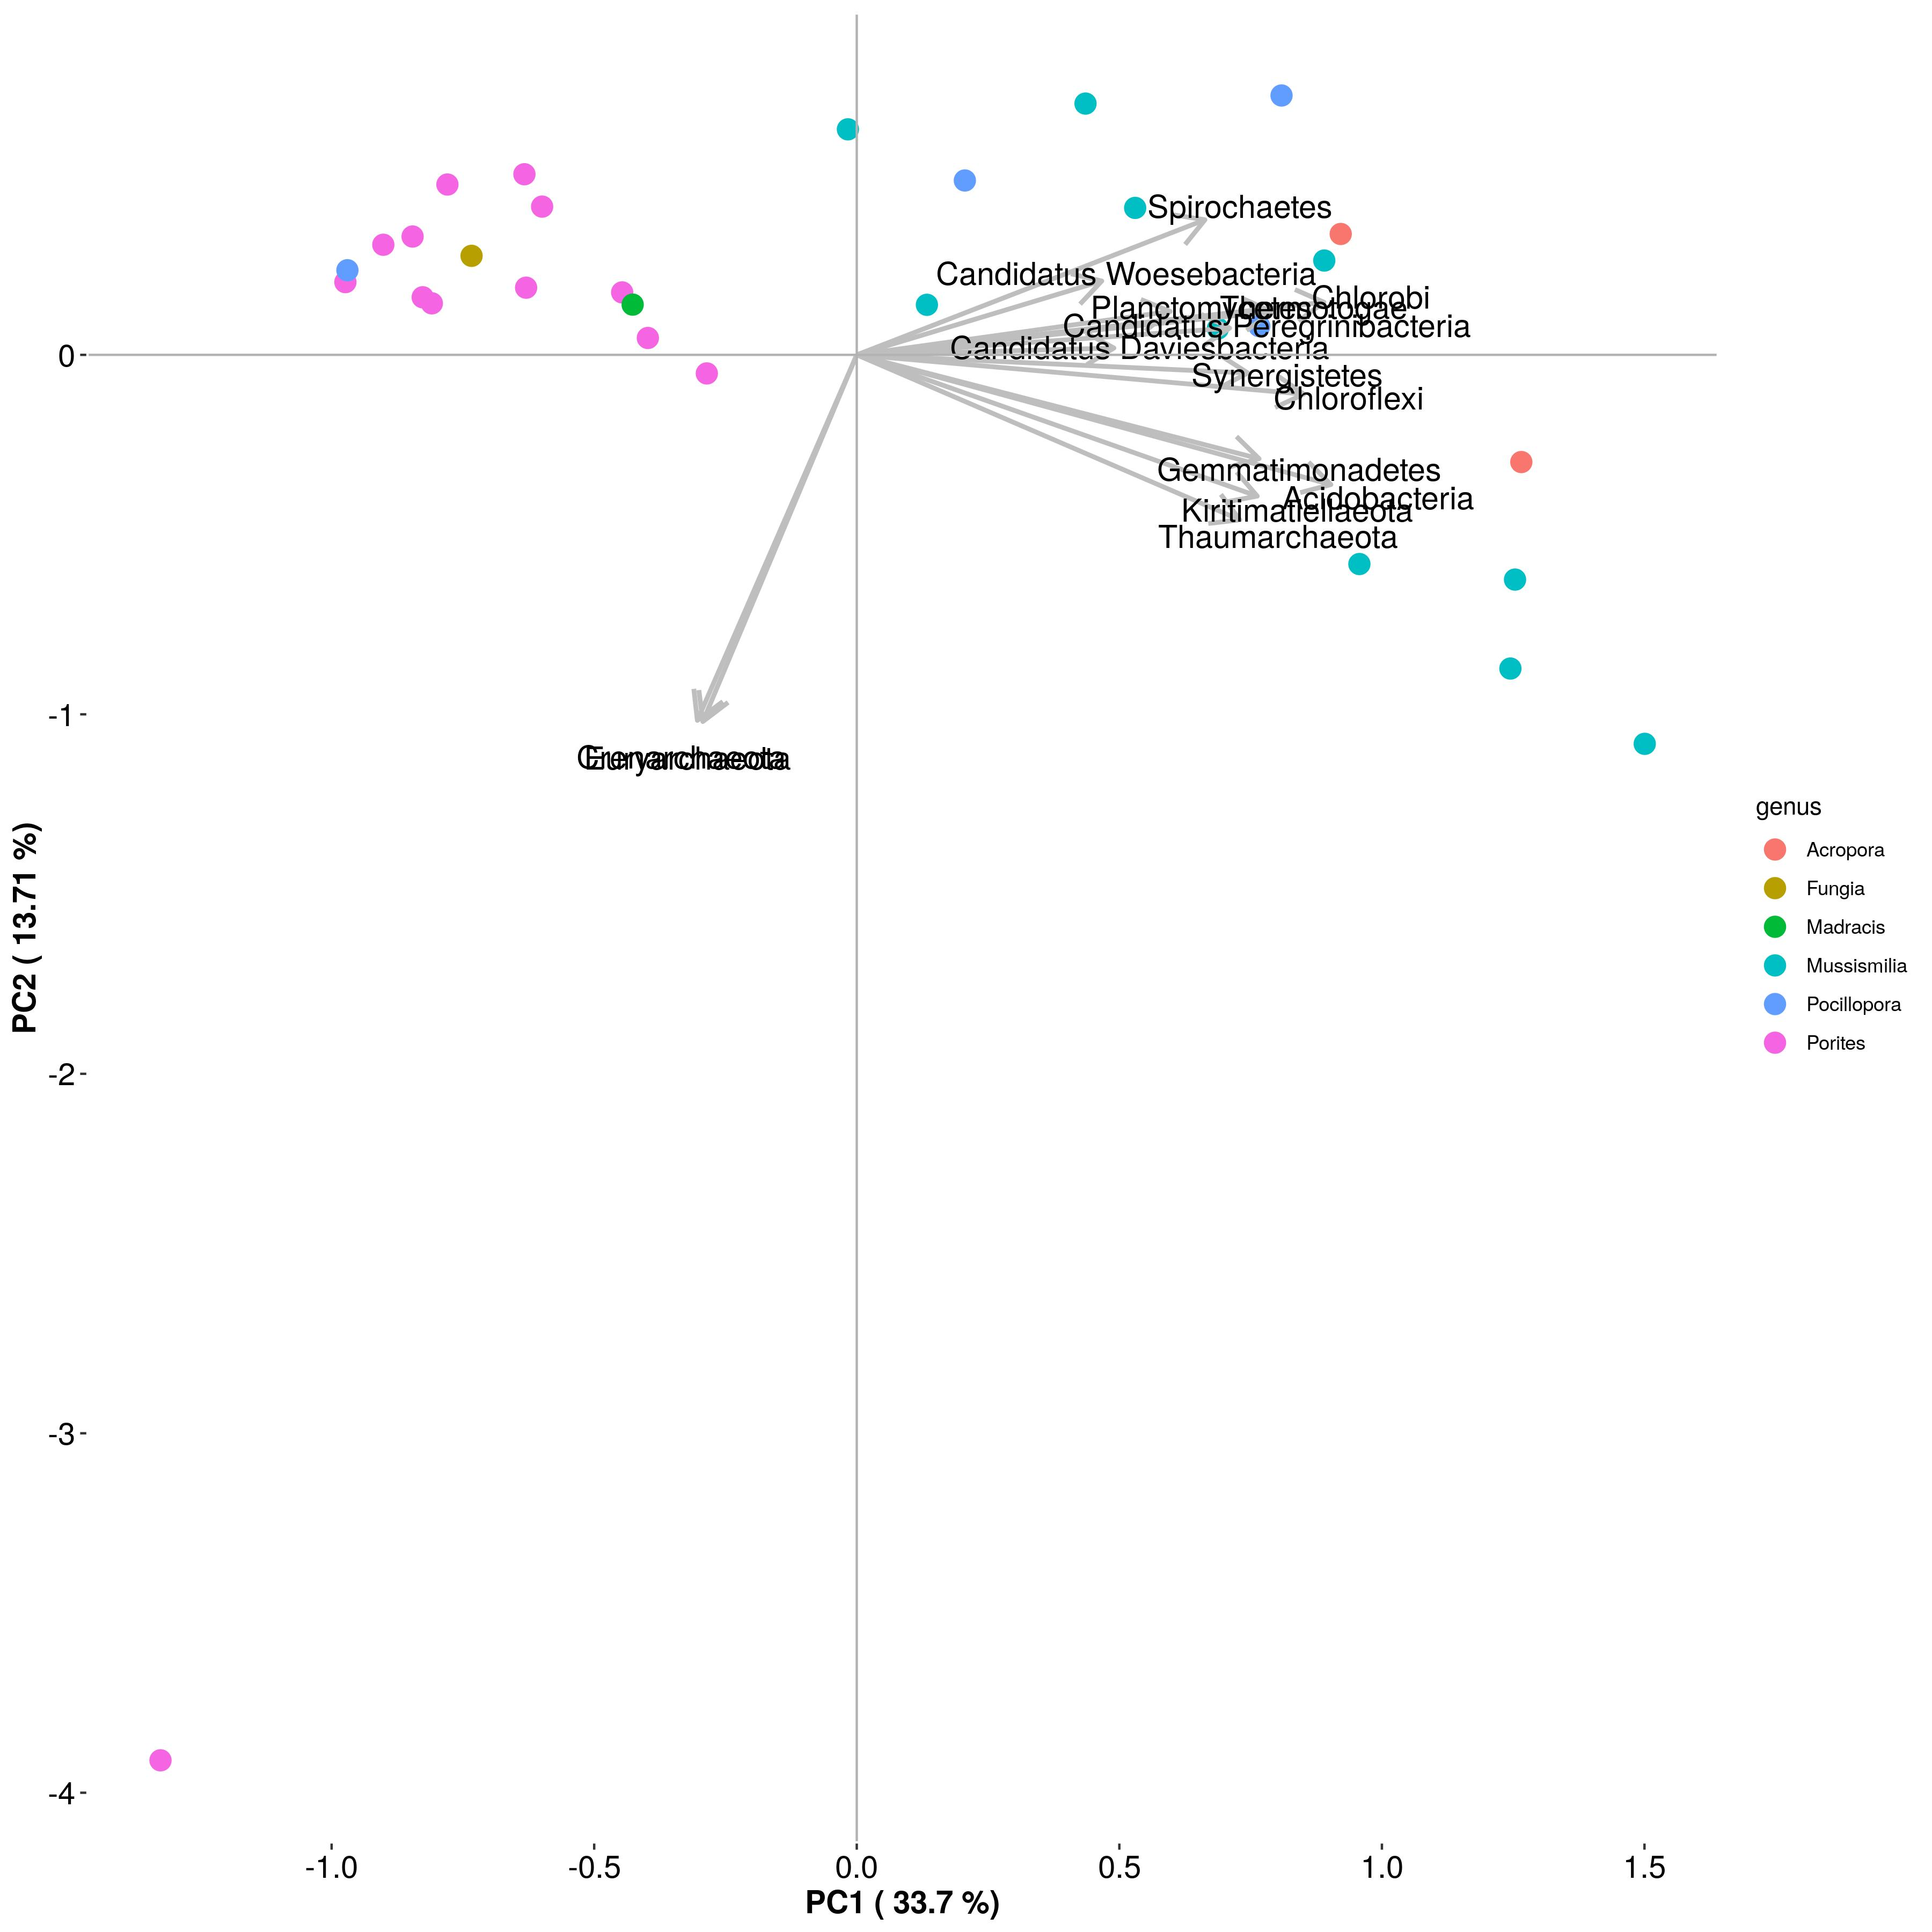
\includegraphics[scale=0.4]{figures/pca_corais_mg_rast_rf_supervisionado_genus_15_filos_23_10_2018.jpg}
\caption{PCA GERADO COM OS PRIMEIROS 15 FILOS DO RANDOM FOREST SUPERVISIONADO POR GENERO}
\end{figure}

\section{Obtencao de figuras 30/10/2018}
O Rilquer sinalizou que a base de dados ainda tinha alguns problemas, entao tive de refazer as analises. Fiz análises para familia e filo. Ordem: \\
\textbf{FILO:}
\begin{itemize}
\item nMDS 
\item PCA geral
\item Random Forest nao supervisionado
\item PCA com os 20 primeiros filos indicados pelo RF nao supervisionado
\item PCA com os 15 primeiros filos  indicados pelo RF nao supervisionado
\item PCA com 10 primeiros filos  indicados pelo RF nao supervisionado
\item Random Forest supervisionado por genero de coral
\item PCA com os 20 primeiros filos  indicados pelo RF supervisionado por genero
\item PCA com os 15 primeiros filos  indicados pelo RF supervisionado por genero
\item PCA com 10 primeiros filos  indicados pelo RF supervisionado por genero
\item Random Forest supervisionado por saude de coral
\item PCA com os 20 primeiros filos  indicados pelo RF supervisionado por saude de coral
\item PCA com os 15 primeiros filos  indicados pelo RF supervisionado por saude de coral
\item PCA com 10 primeiros filos  indicados pelo RF supervisionado por saude de coral
\end{itemize}

\textbf{FAMILIA:}
\begin{itemize}
\item nMDS 
\item PCA geral
\item \textbf{Random Forest nao supervisionado}
\item PCA com os 20 primeiras familias indicados pelo RF nao supervisionado
\item PCA com os 15 primeiras familias  indicados pelo RF nao supervisionado
\item PCA com 10 primeiros familias indicados pelo RF nao supervisionado
\item \textbf{Random Forest supervisionado por genero de coral}
\item PCA com os 20 primeiros familias  indicados pelo RF supervisionado por genero
\item PCA com os 15 primeiros familias  indicados pelo RF supervisionado por genero
\item PCA com 10 primeiros familias  indicados pelo RF supervisionado por genero
\item \textbf{Random Forest supervisionado por saude de coral}
\item PCA com os 20 primeiros familias  indicados pelo RF supervisionado por saude de coral
\item PCA com os 15 primeiros familias  indicados pelo RF supervisionado por saude de coral
\item PCA com 10 primeiros familias  indicados pelo RF supervisionado por saude de coral
\end{itemize}

\subsection{FILO}
\begin{figure}[H]
\centering
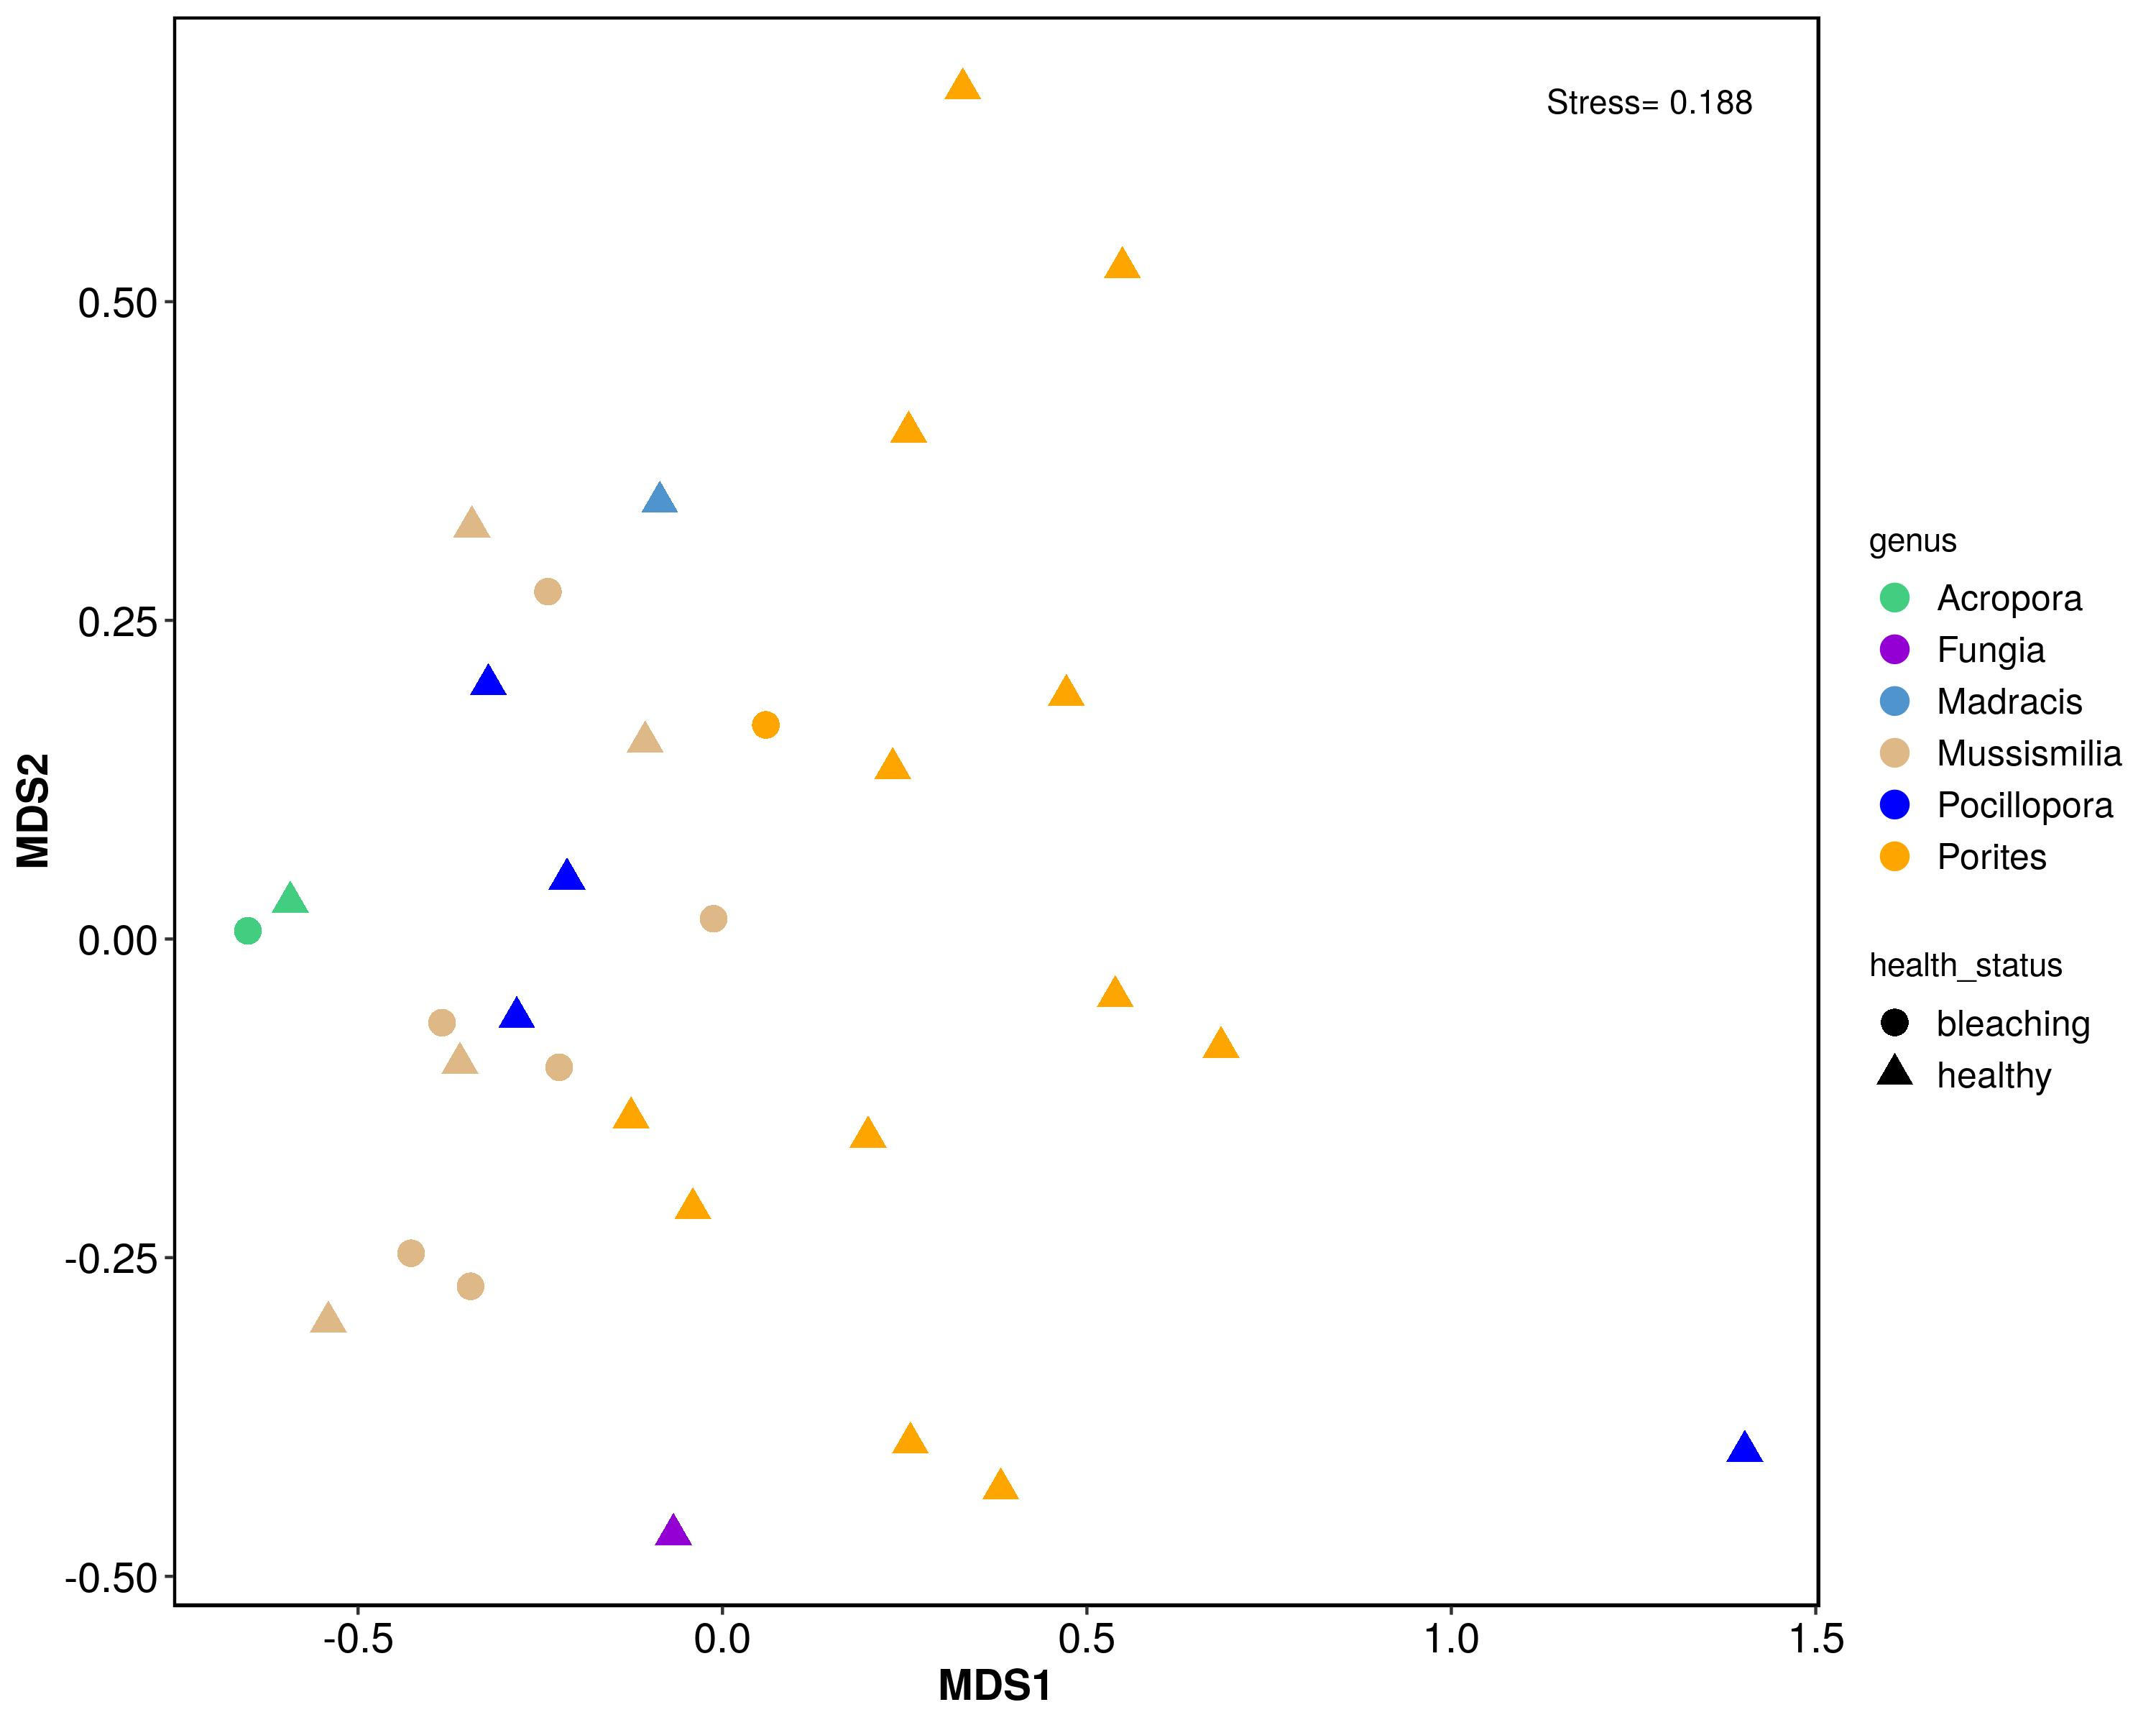
\includegraphics[scale=0.4]{figures/filos/nMDS_filos_corais_2018_10_30.jpg}
\caption{nMDS feito com matriz de abundancia de filos}
\label{fig:nMDSfeito30deoutubro}
\end{figure}

\begin{figure}[H]
\centering
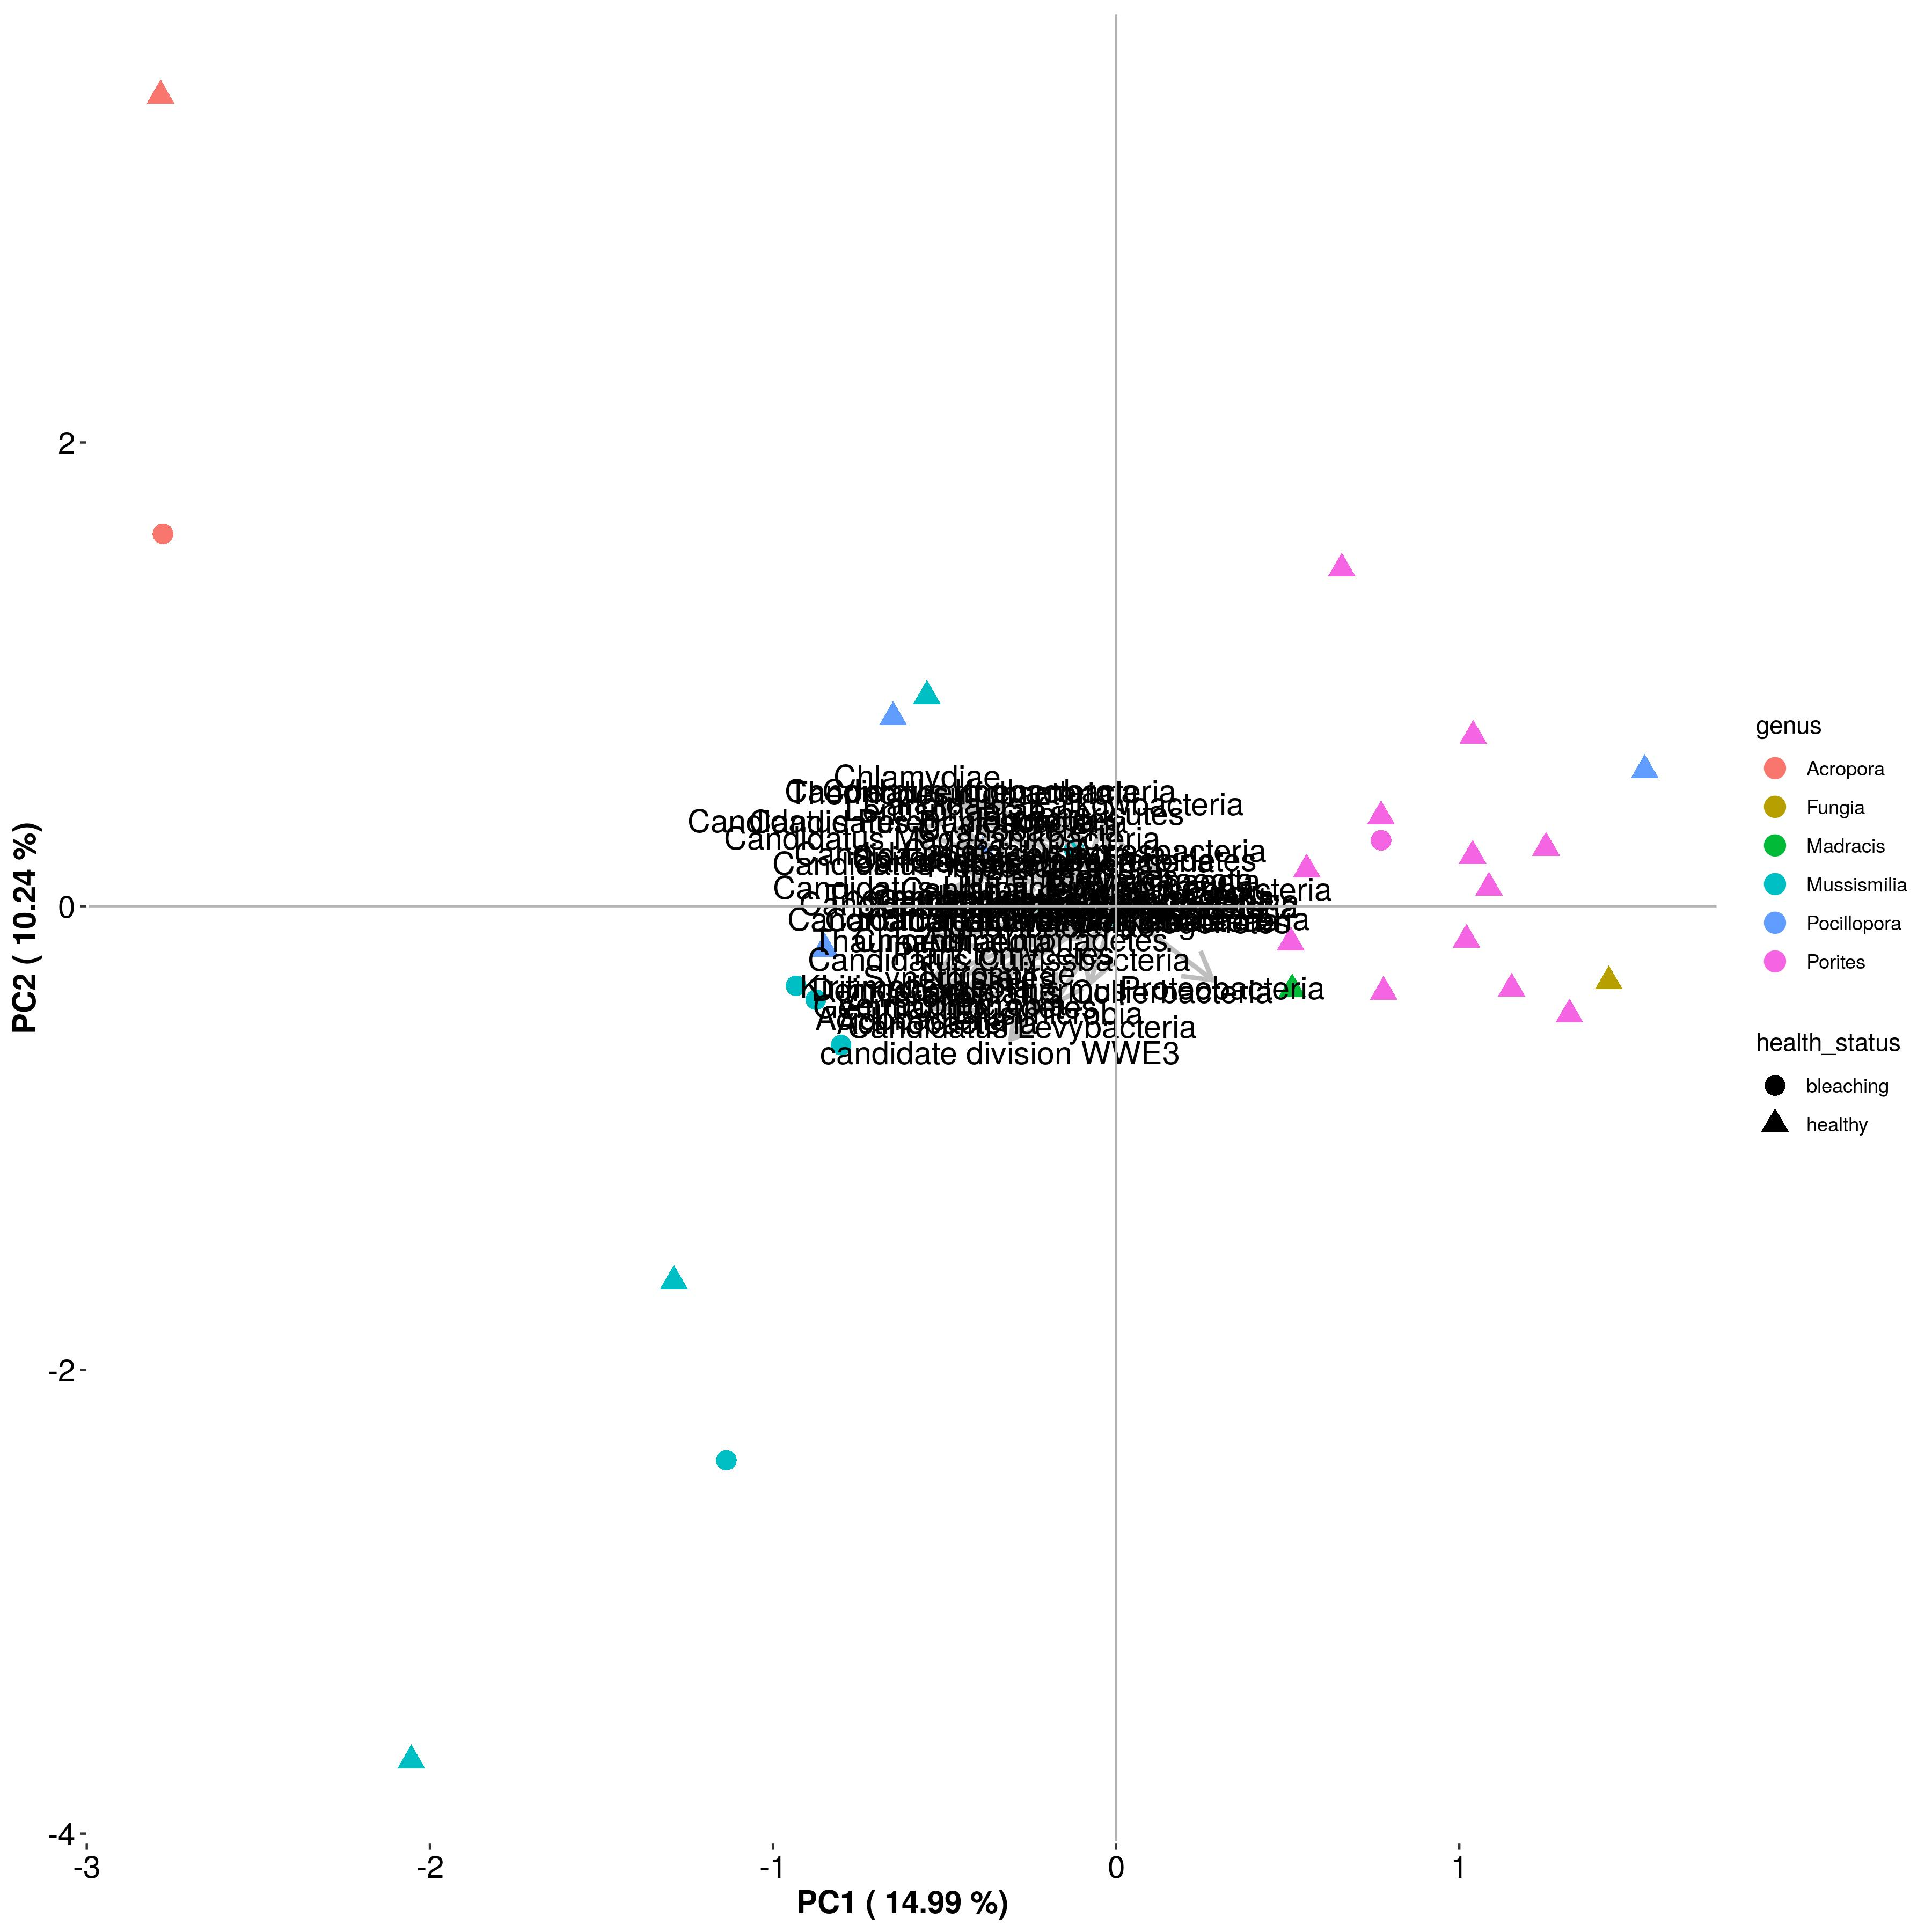
\includegraphics[scale=0.4]{figures/filos/output_PCA_corais_filos_mg_rast_2018_10_30.jpg}
\caption{PCA geral feito com matriz de abundancia de filos}
\label{fig:PCAfeito30deoutubro}
\end{figure}

\begin{figure}[H]
\centering
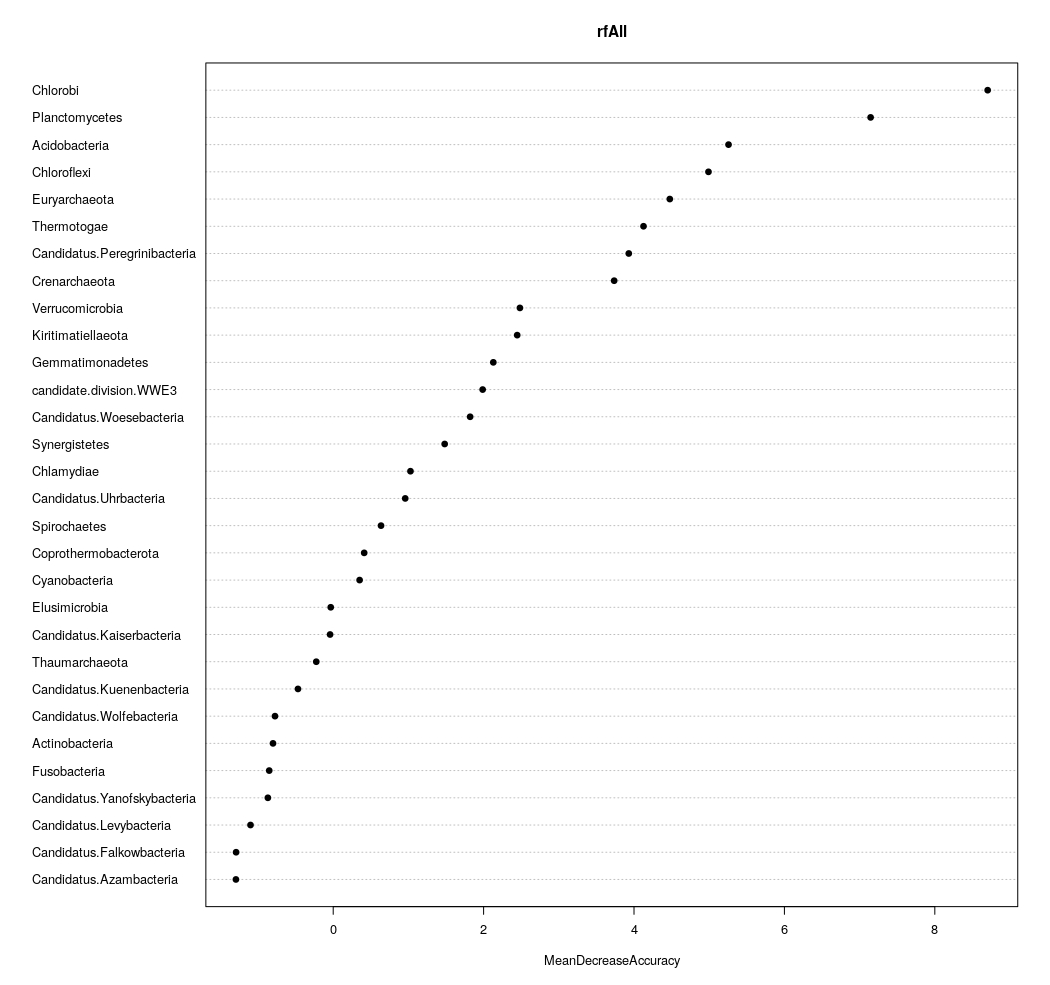
\includegraphics[scale=0.4]{figures/filos/randomforest_nao_supervisionado_corais_mgrast_filos_leticia_2018_10_30.jpeg}
\caption{RANDOM FOREST NÃO SUPERVISIONADO DAS AMOSTRAS DE CORAIS DO MG RAST FEITO DIA 30 DE OUTUBRO}
\label{fig:Rfnaosupervisionadofeito30deoutubro}
\end{figure}

\begin{figure}[H]
\centering
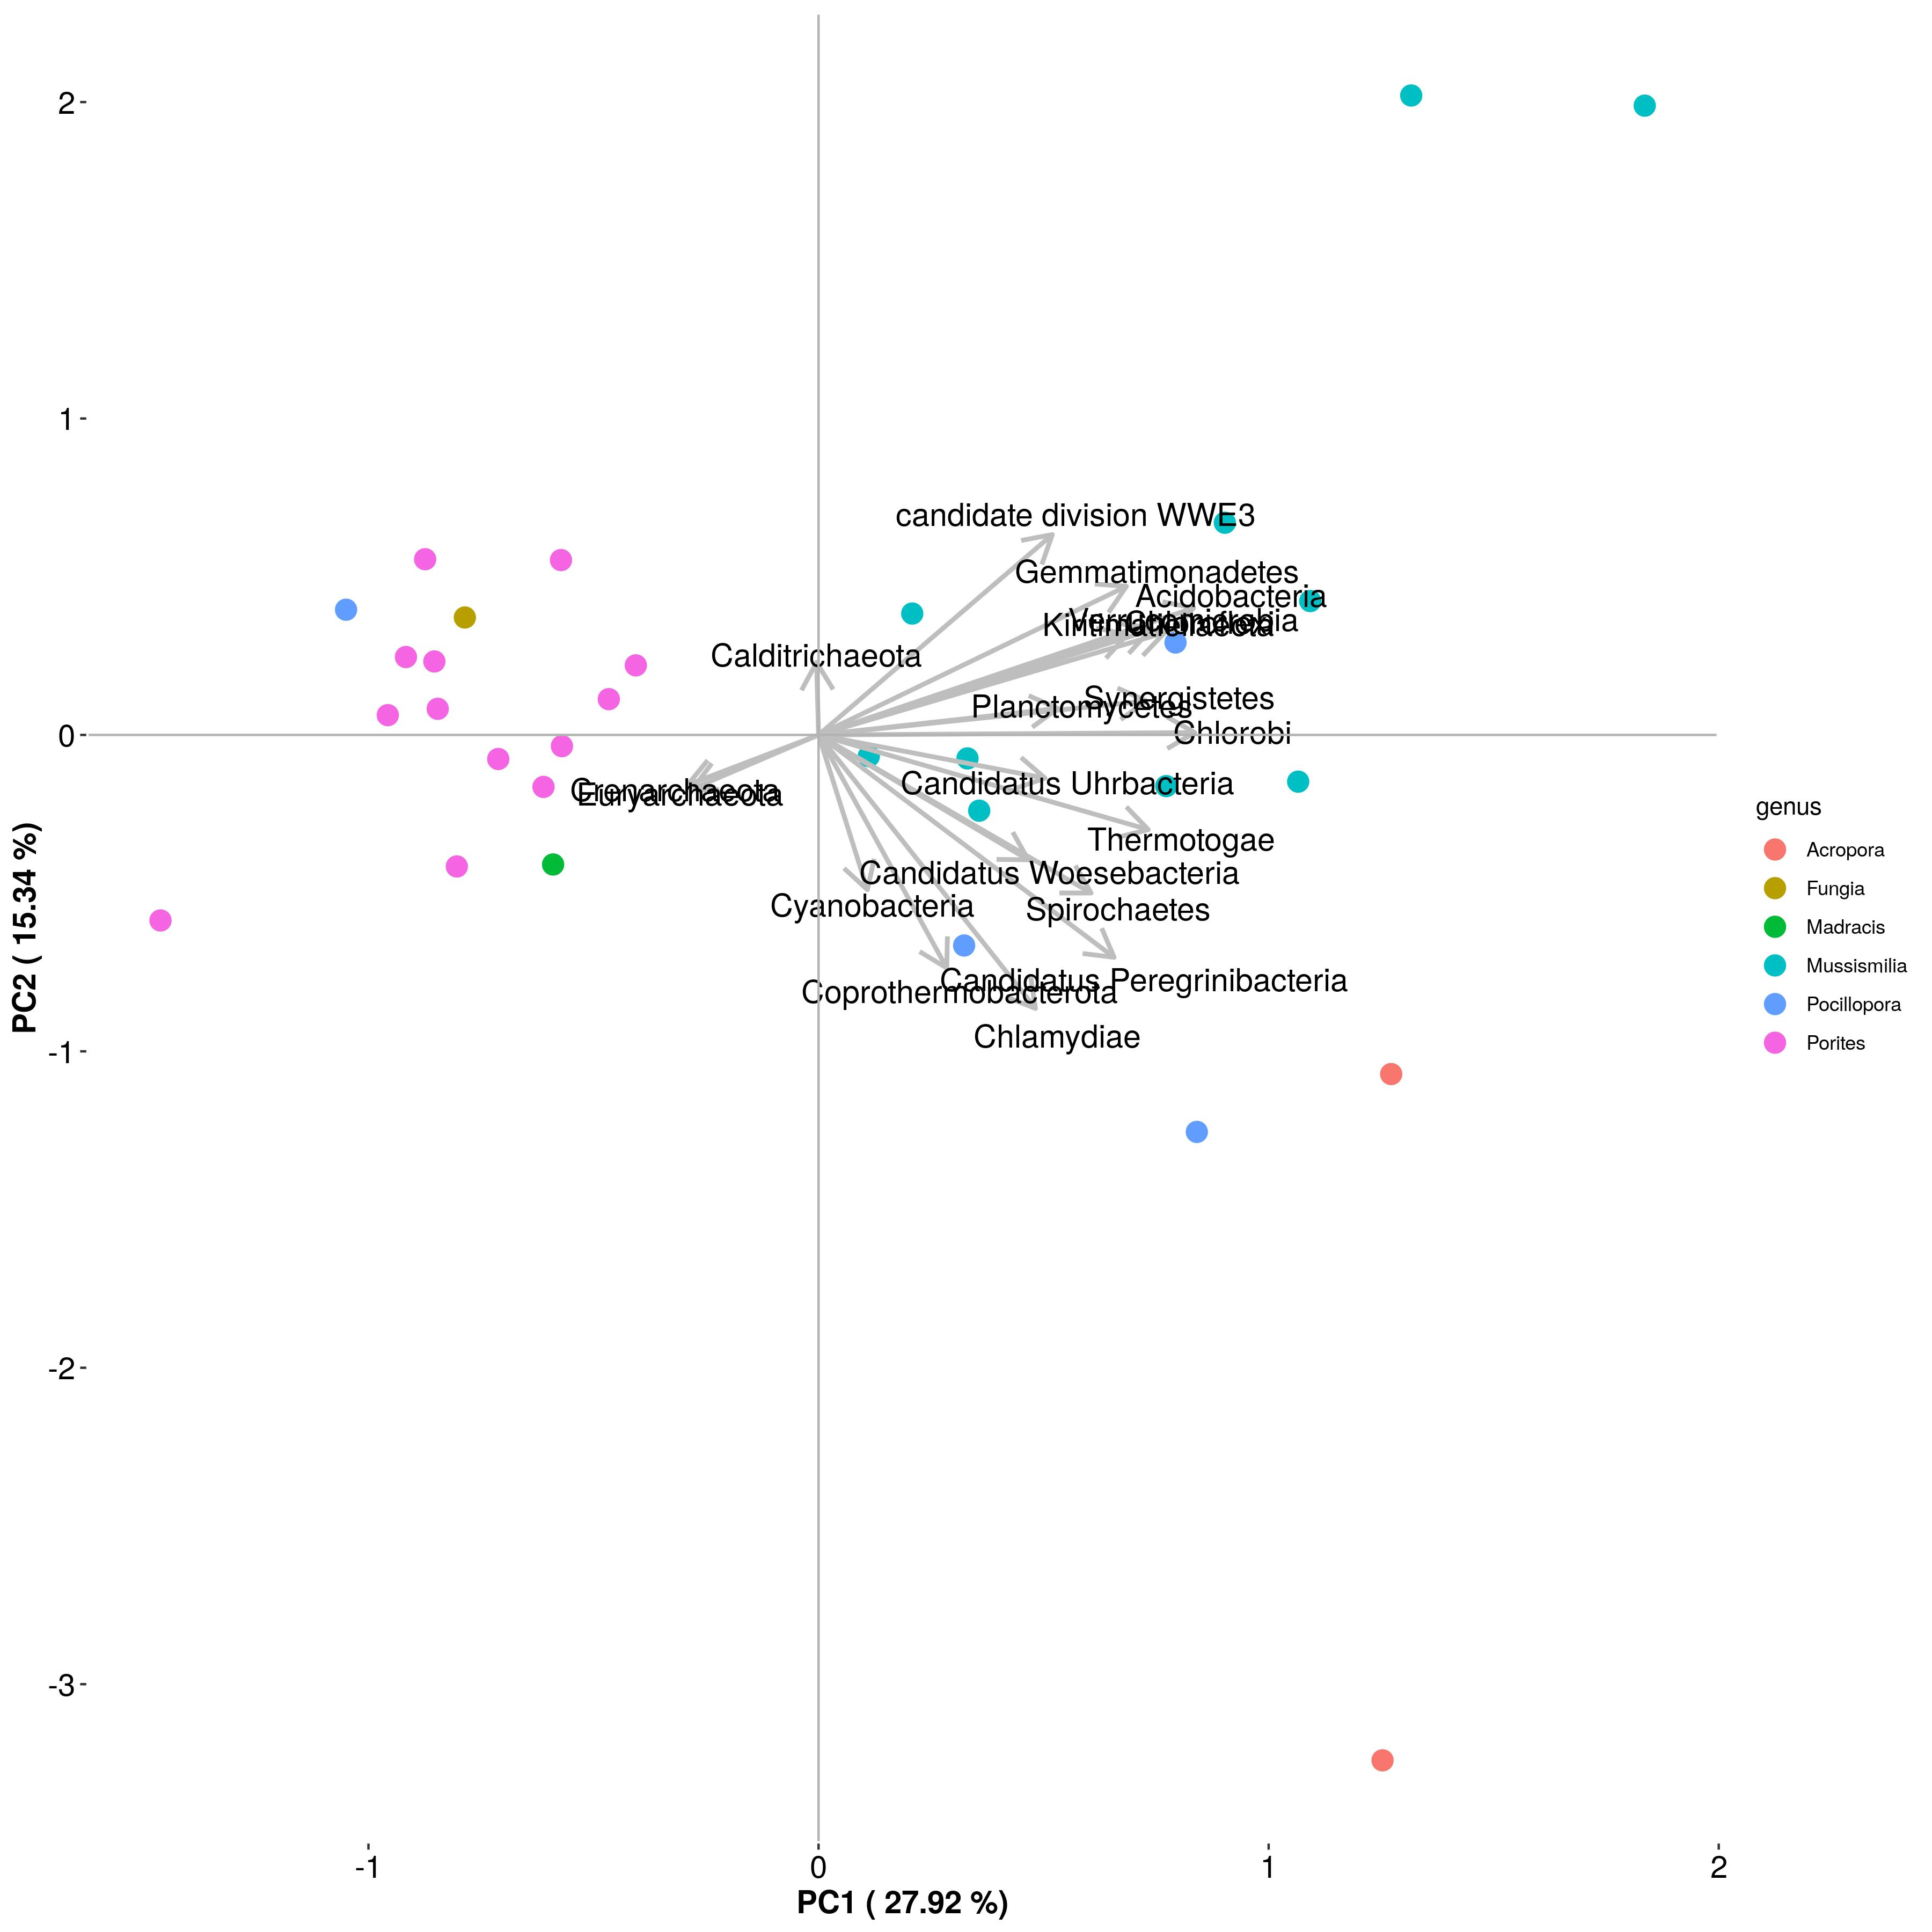
\includegraphics[scale=0.3]{figures/filos/pca_corais_mgrast_rf_nao_supervisionado_20_filos_30_10_2018.jpg}
\caption{PCA feito com os 20 primeiros filos indicados pelo Random Forest não supervisionado 30 DE OUTUBRO}
\label{fig:PCAcom20filosderivadodoRfnaosupervisionadofeito30deoutubro}
\end{figure}

\begin{figure}[H]
\centering
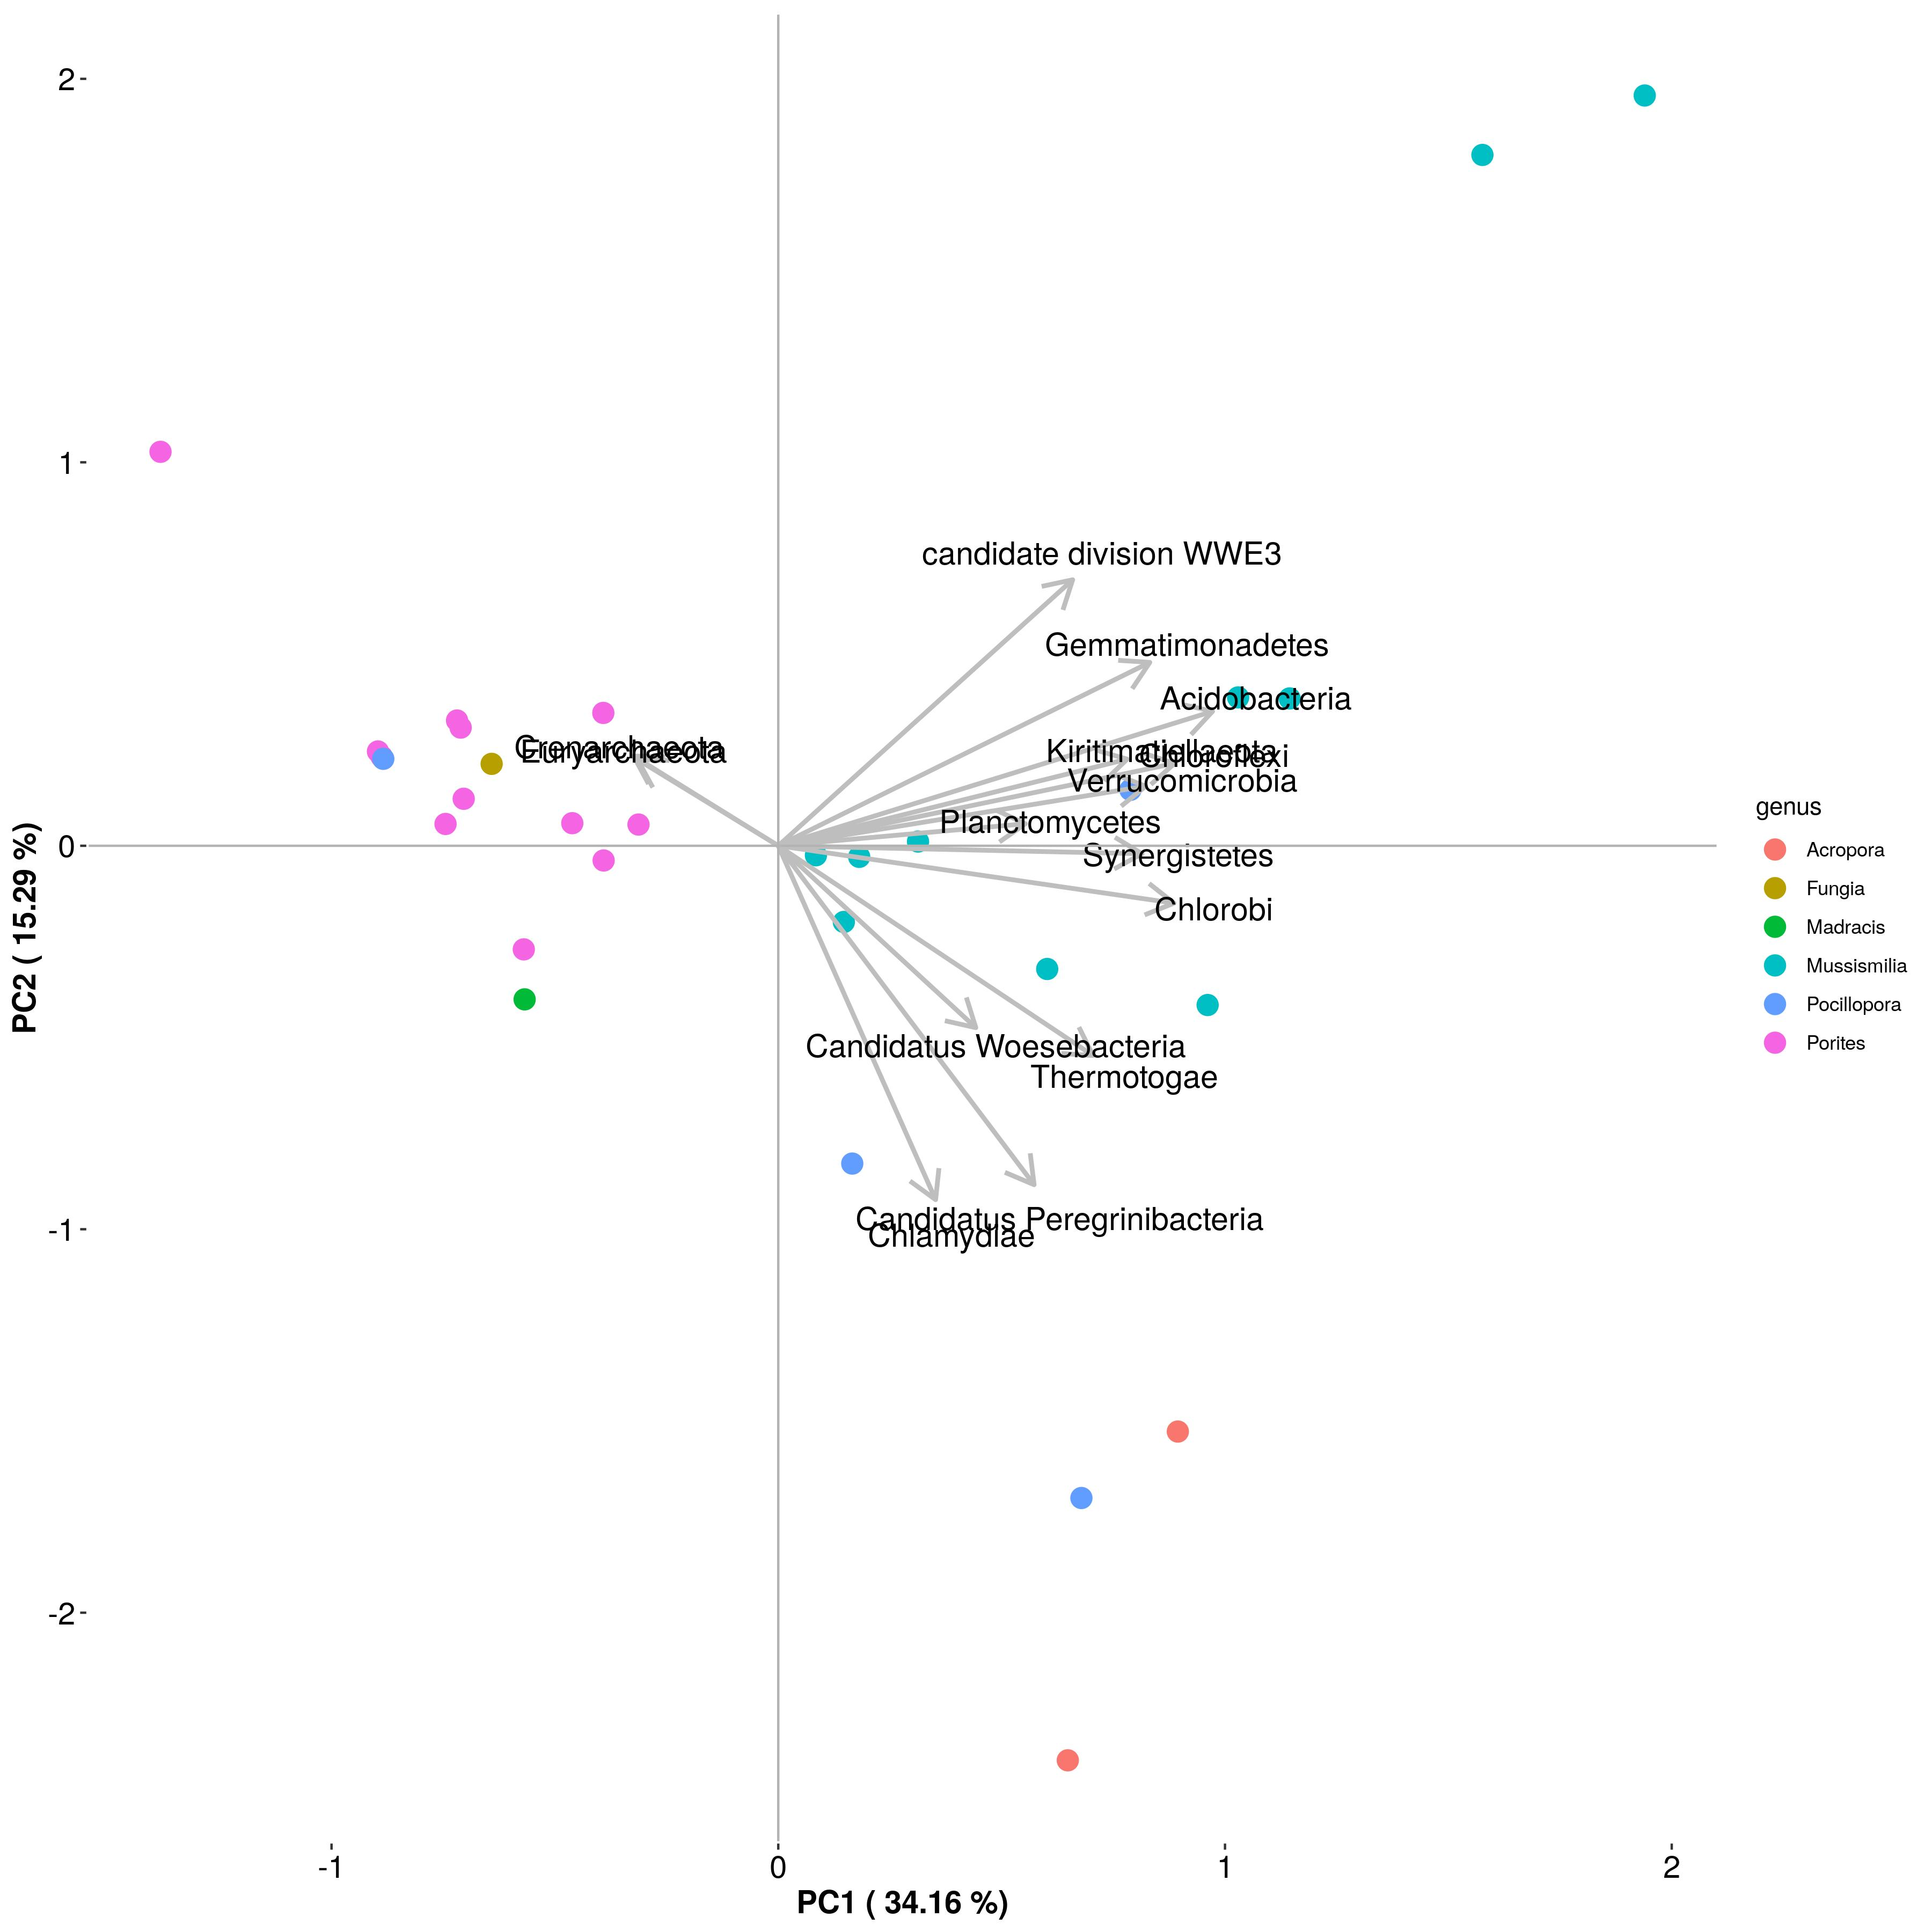
\includegraphics[scale=0.3]{figures/filos/pca_corais_mgrast_rf_nao_supervisionado_15_filos_30_10_2018.jpg}
\caption{PCA feito com os 15 primeiros filos indicados pelo Random Forest não supervisionado 30 DE OUTUBRO}
\label{fig:PCAcom15filosderivadodoRfnaosupervisionadofeito30deoutubro}
\end{figure}

\begin{figure}[H]
\centering
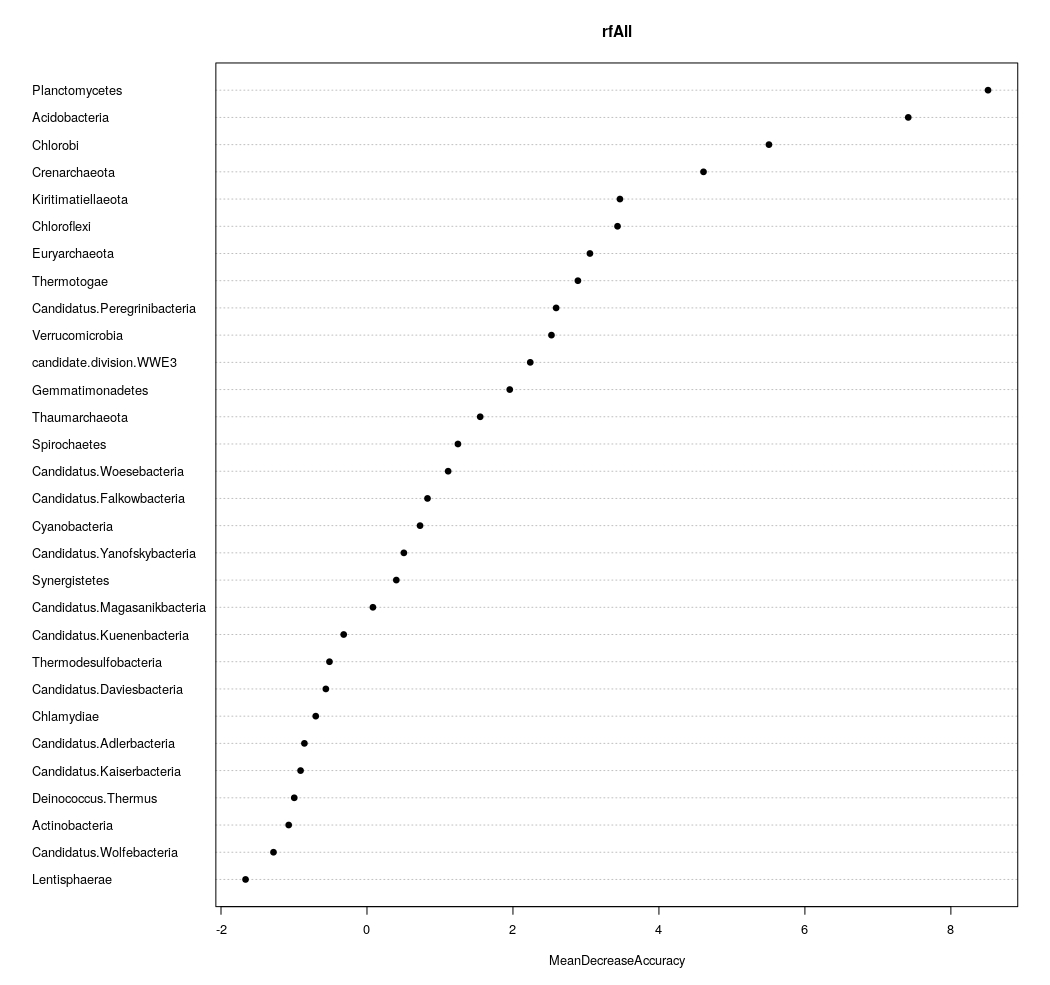
\includegraphics[scale=0.4]{figures/filos/randomforest_supervisionado_genero_corais_mgrast_leticia_2018_10_30.jpeg}
\caption{Random Forest supervisionado por genero de coral feito 30 de novembro}
\label{fig:RandomForestsupervisionadoporgenerodecoral}
\end{figure}

\begin{figure}[H]
\centering
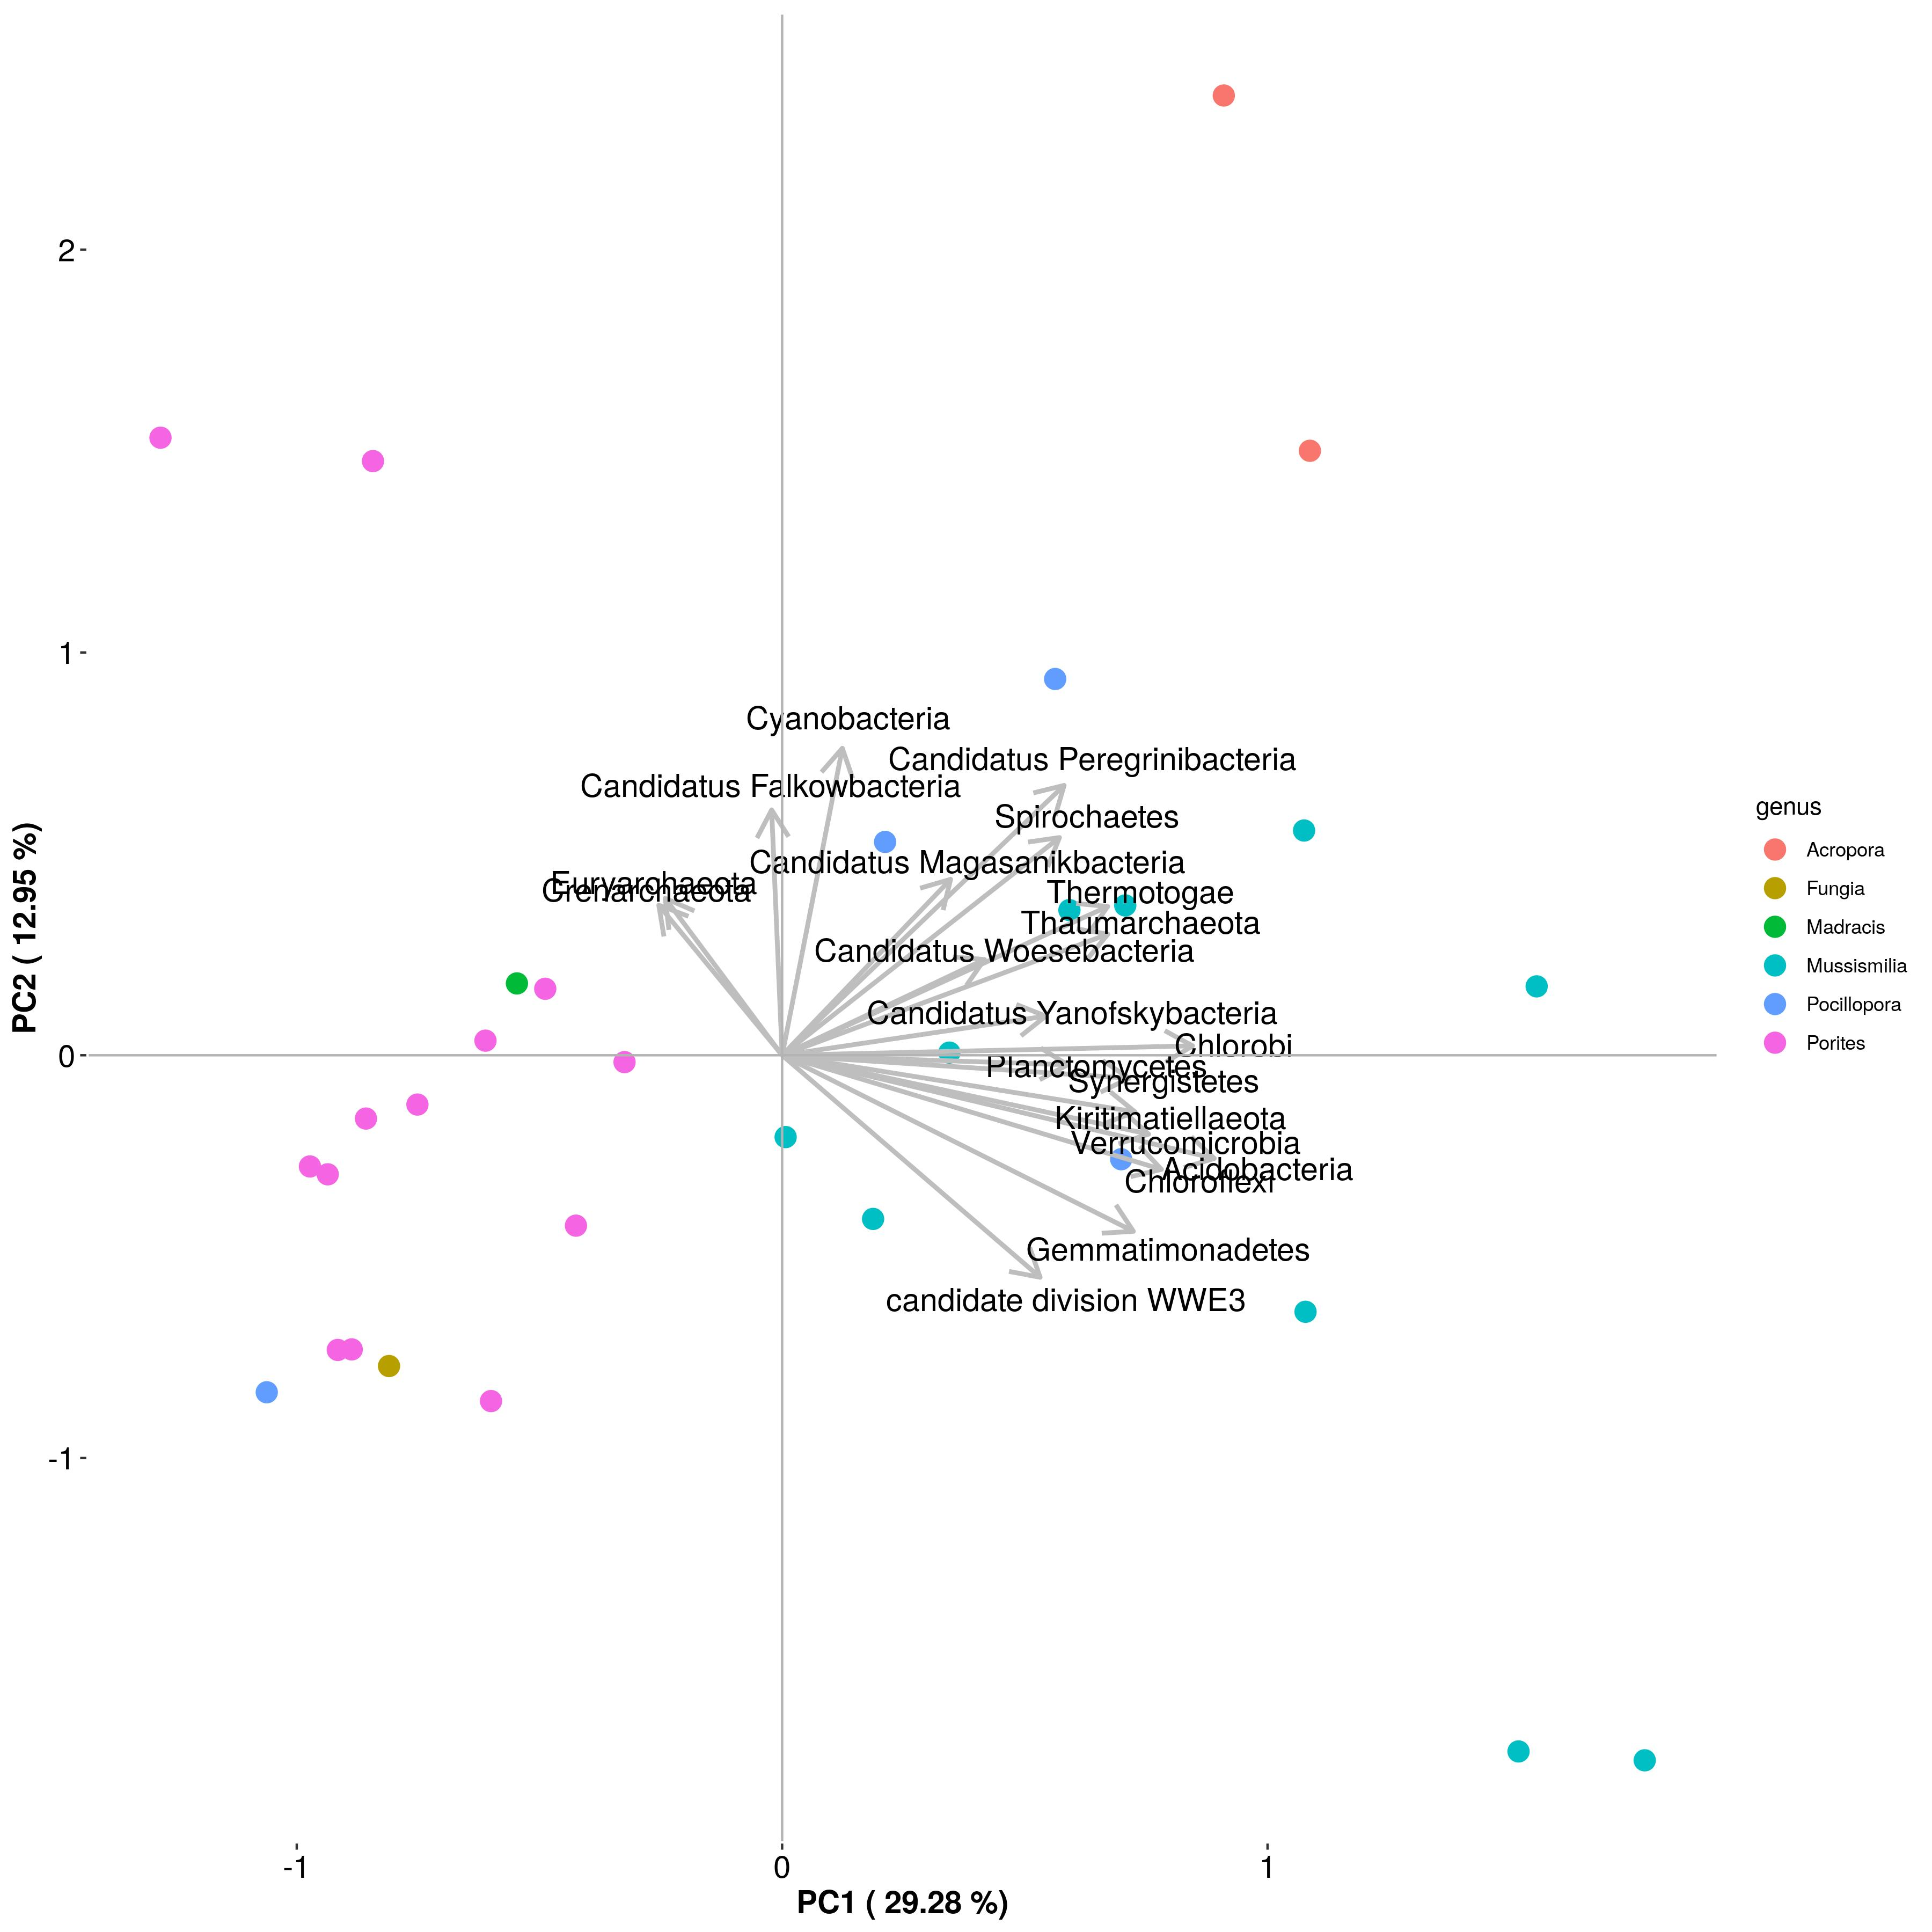
\includegraphics[scale=0.3]{figures/filos/pca_corais_mg_rast_rf_supervisionado_genus_20_filos_30_10_2018.jpg}
\caption{PCA com 20 filos indicados pelo Random Forest supervisionado por genero de coral feito 30 de novembro}
\label{fig:PCAfeitocom20filosrandomForestsupervisionadoporgenerodecoral}
\end{figure}

\begin{figure}[H]
\centering
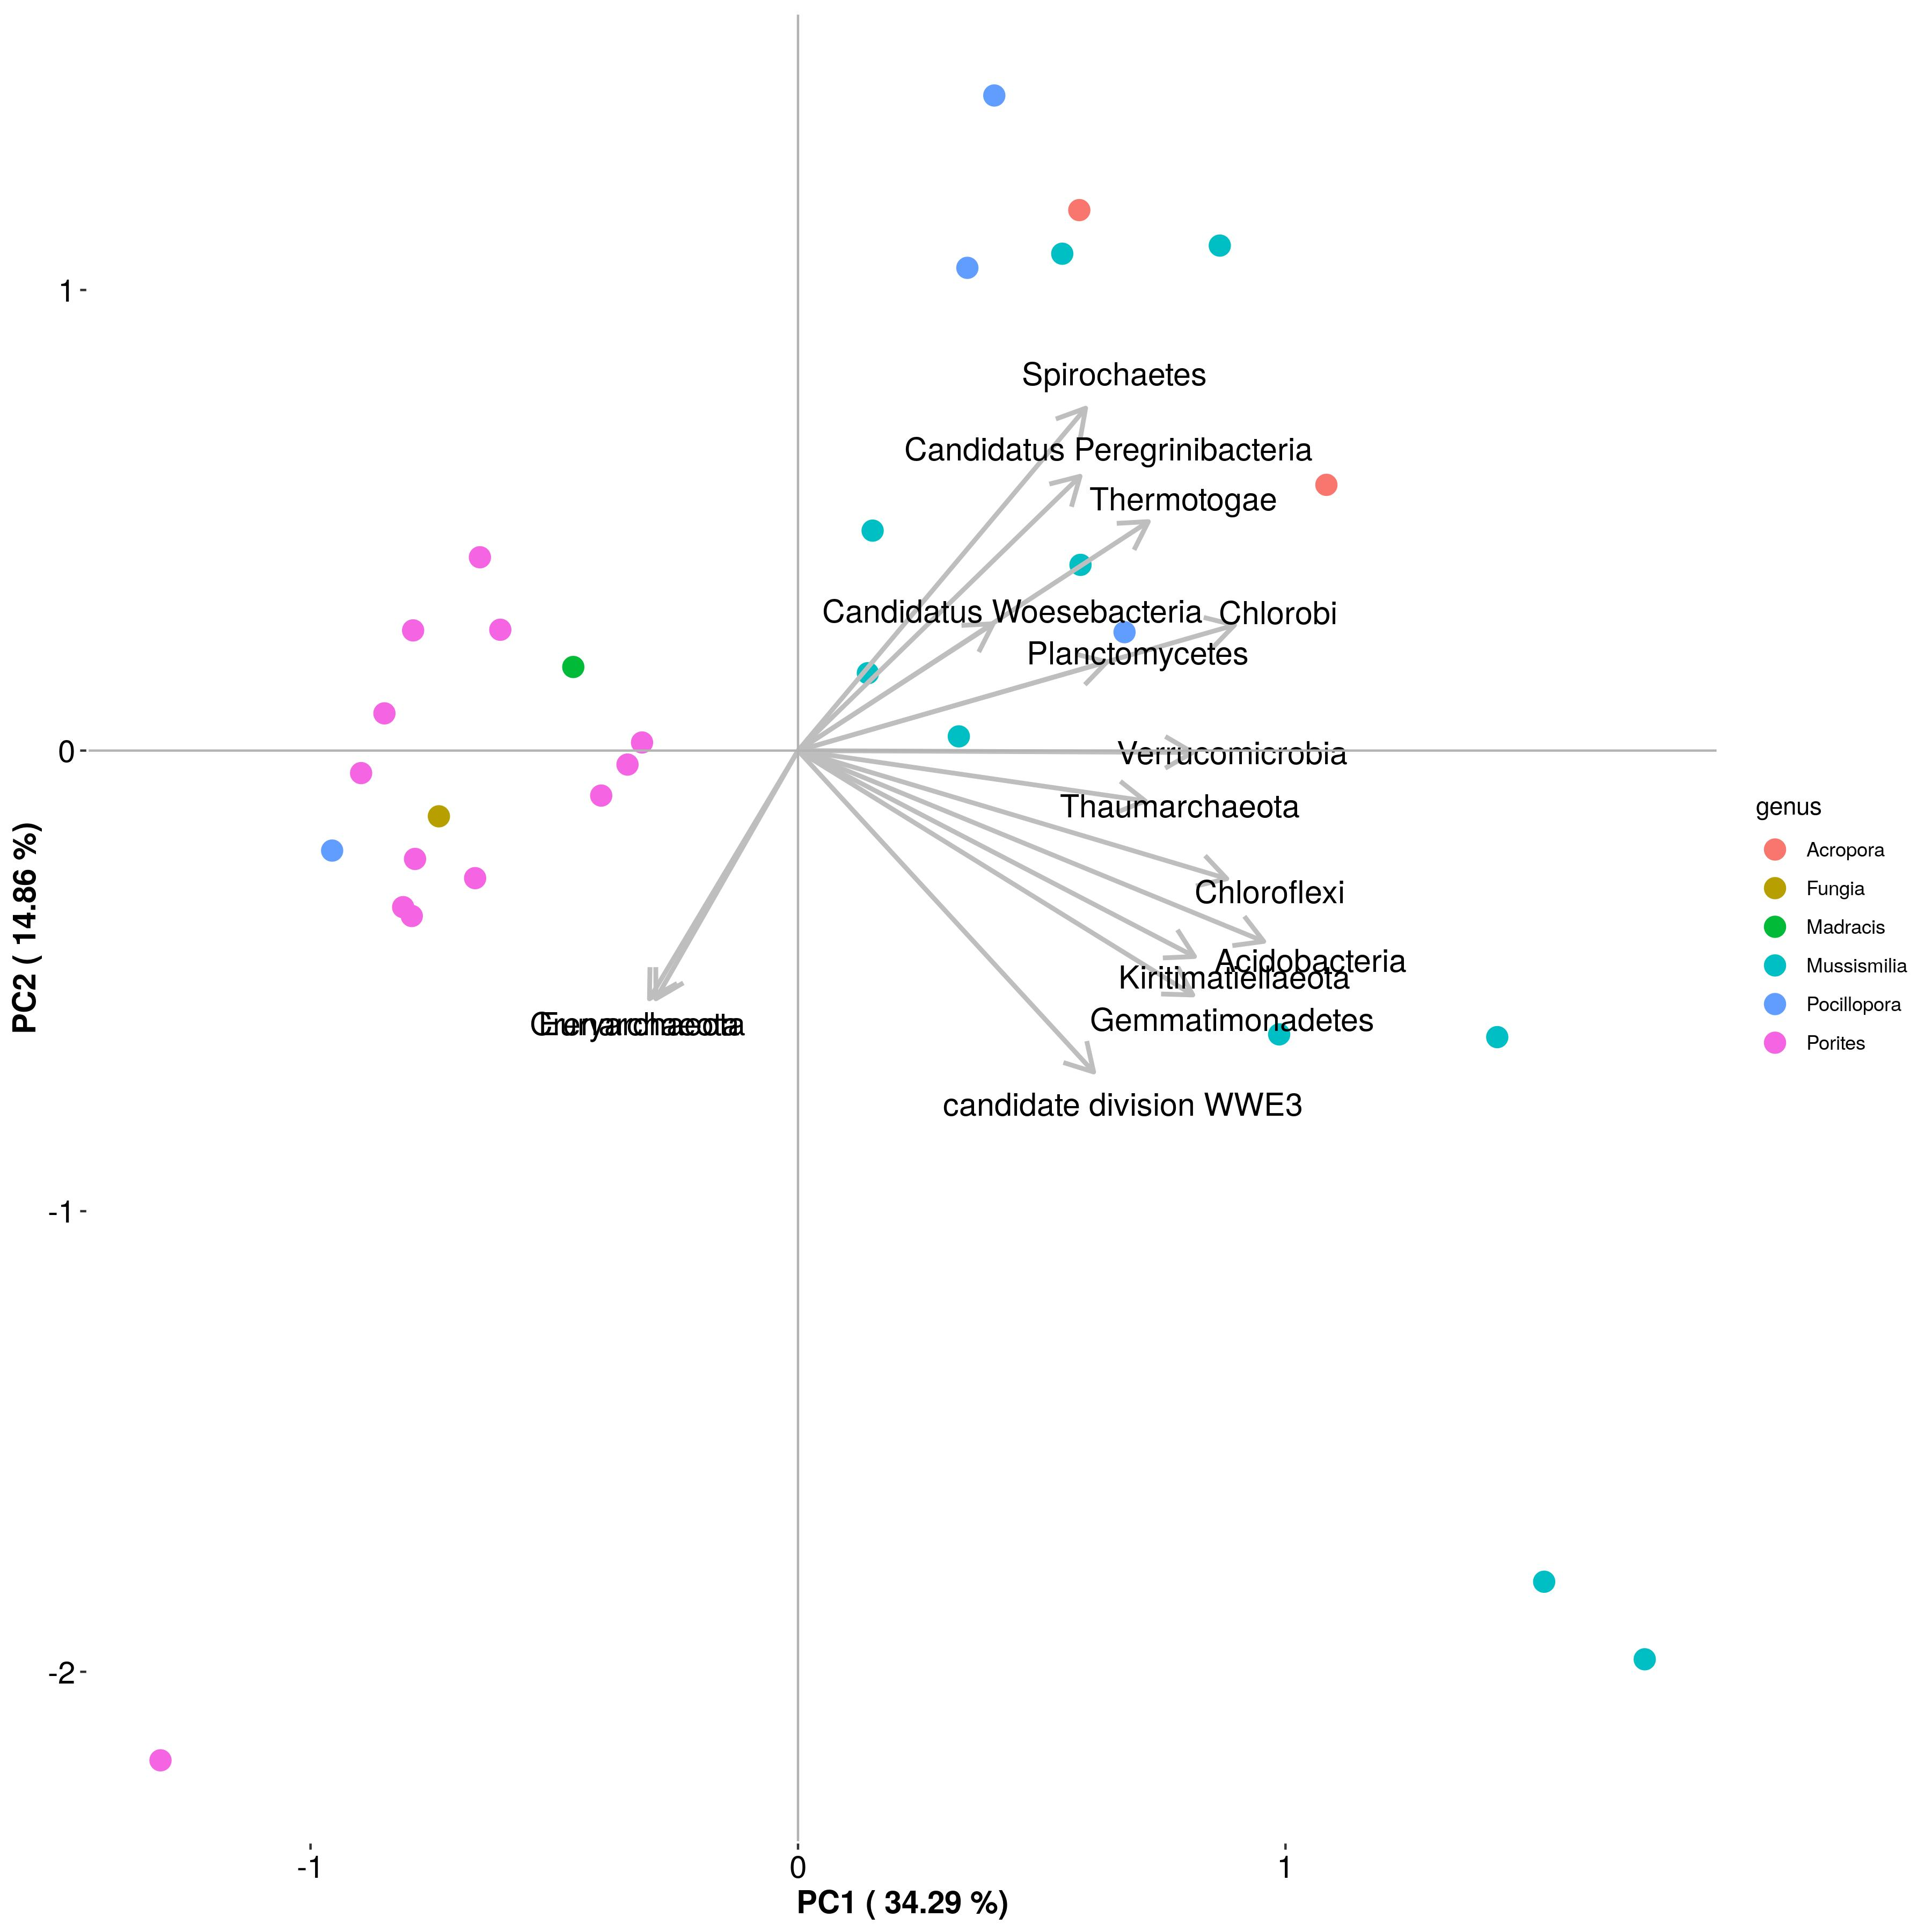
\includegraphics[scale=0.4]{figures/filos/pca_corais_mg_rast_rf_supervisionado_genus_15_filos_30_10_2018.jpg}
\caption{PCA com 15 filos indicados pelo Random Forest supervisionado por genero de coral feito 30 de novembro}
\label{fig:PCAfeitocom15filosrandomForestsupervisionadoporgenerodecoral}
\end{figure}

\subsection{FAMILIA}
\begin{figure}[H]
\centering
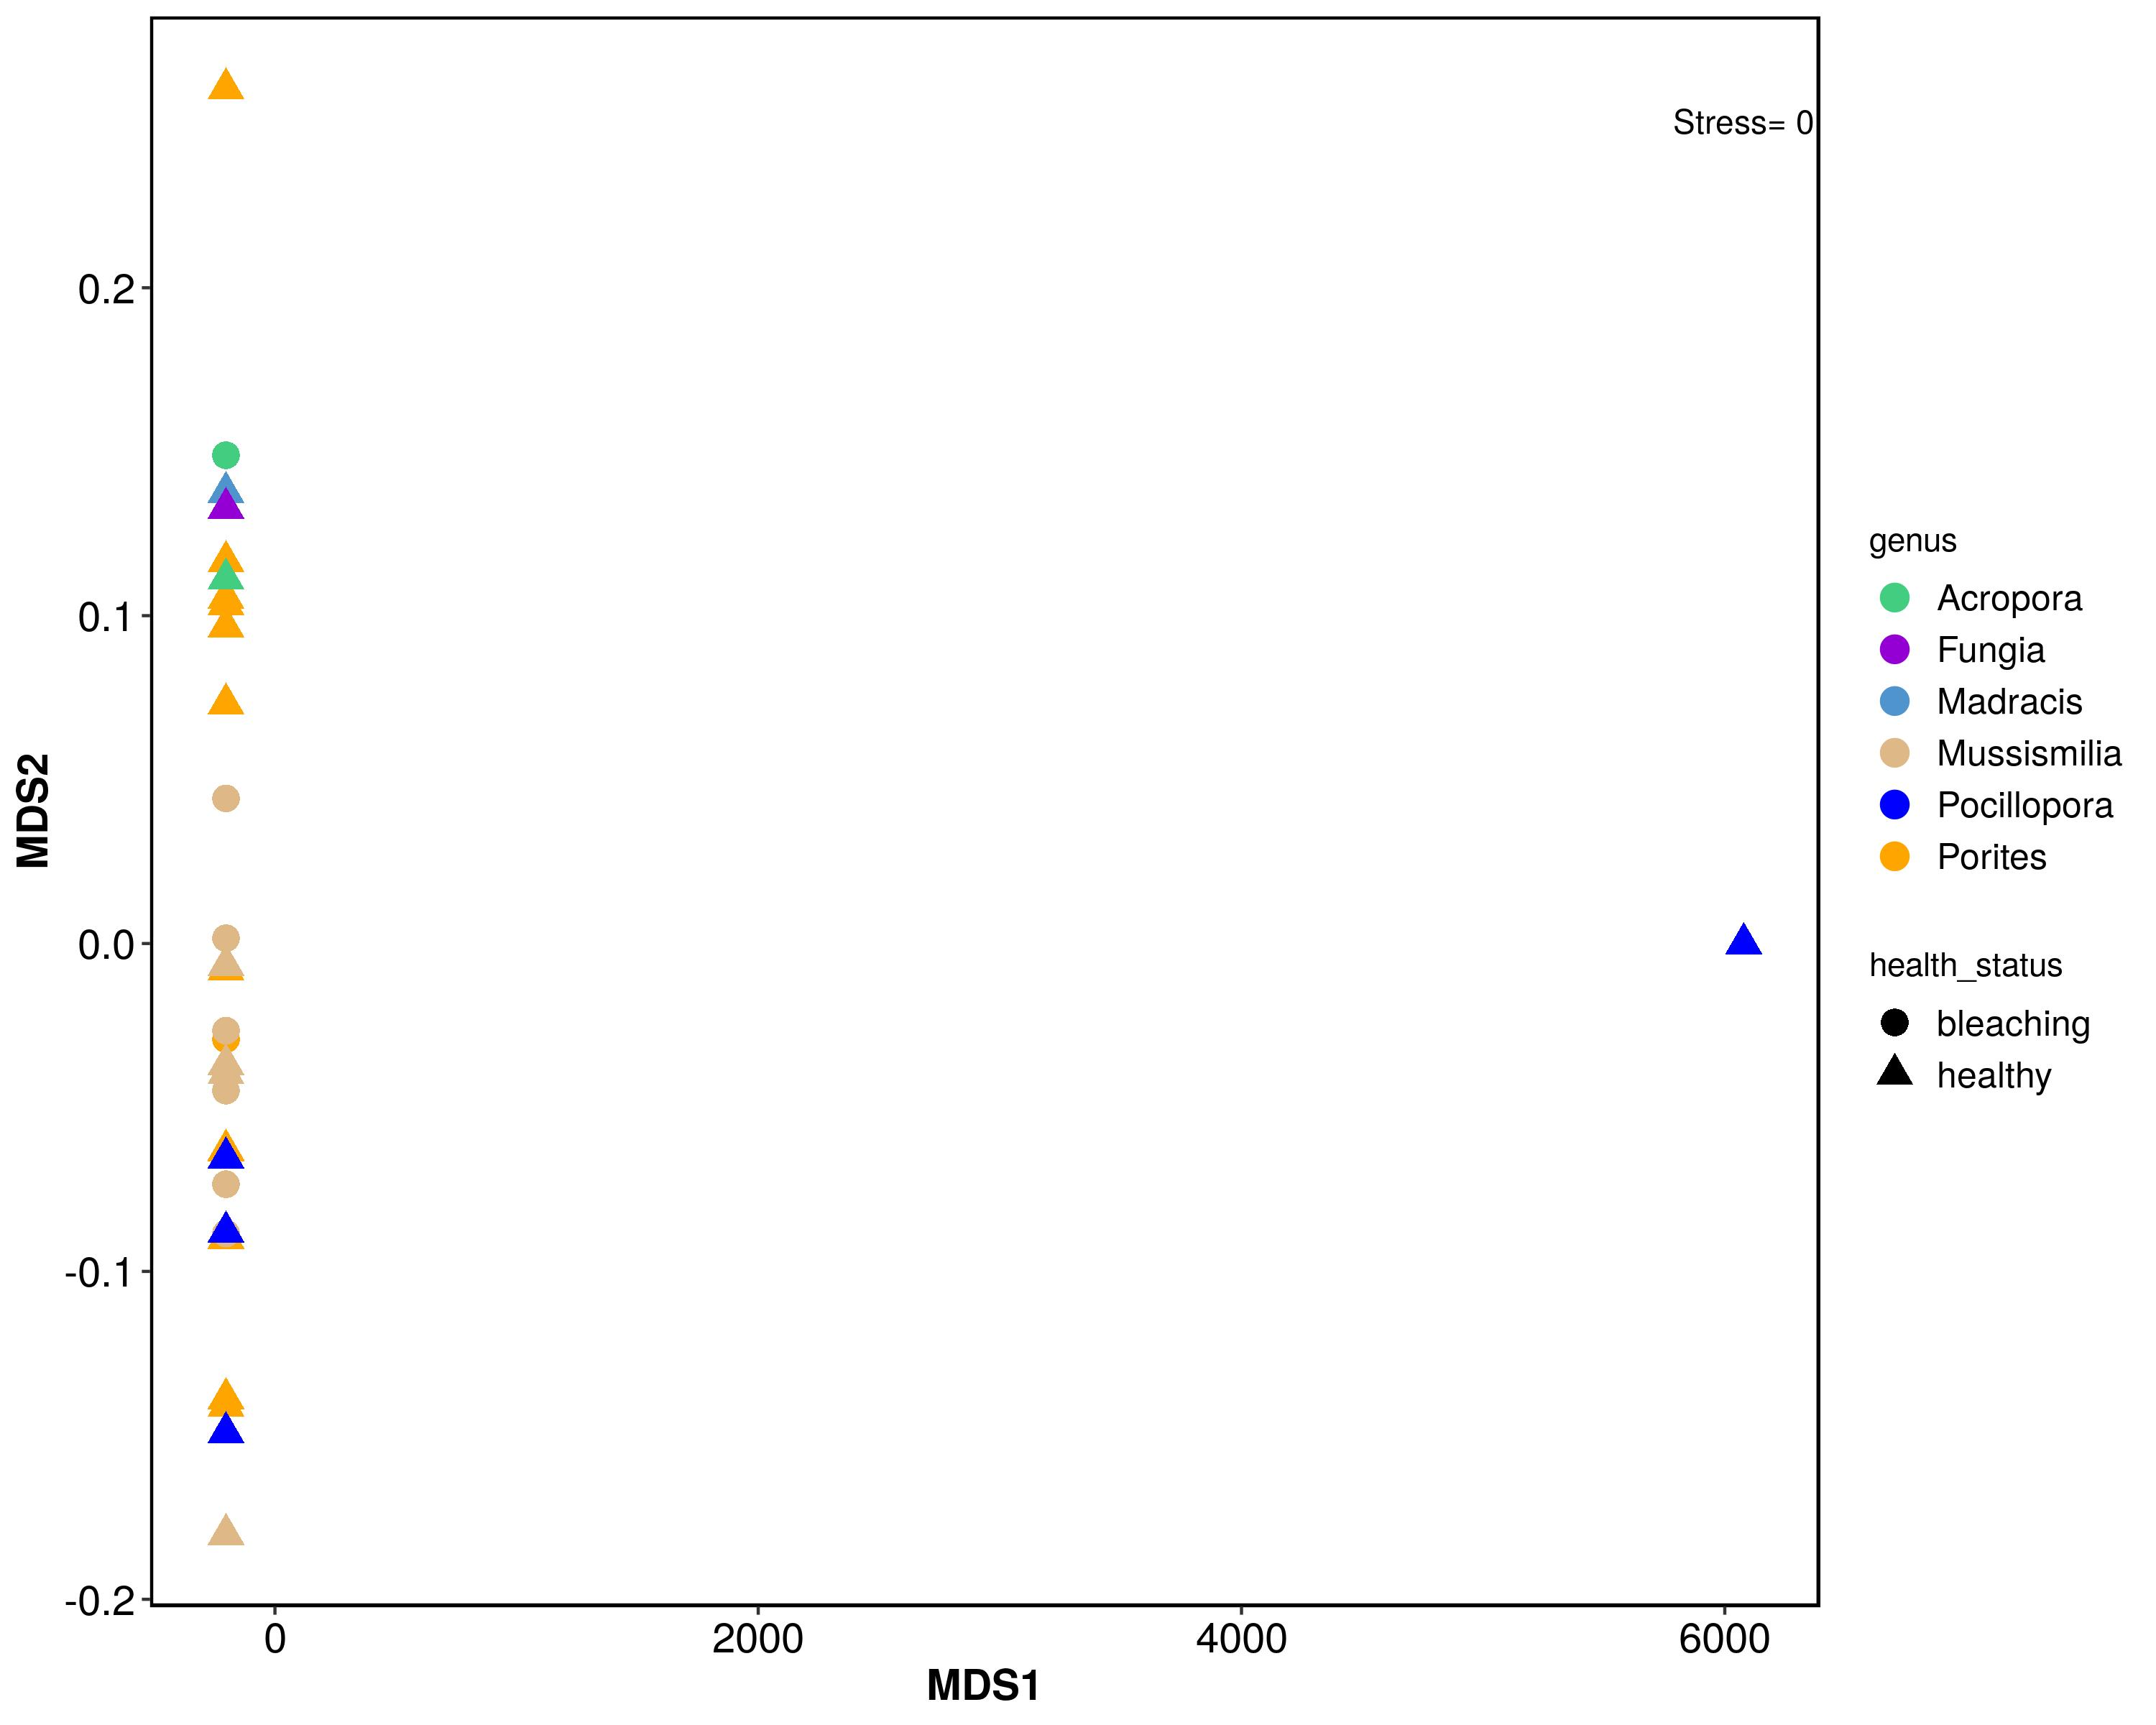
\includegraphics[scale=0.4]{figures/familia/nMDS_taxonomic_family_corais_2018_10_30.jpg}
\caption{nMDS feito com matriz de abundancia de familias}
\label{fig:nMDSfeito30deoutubroparafamilia}
\end{figure}

\begin{figure}[H]
\centering
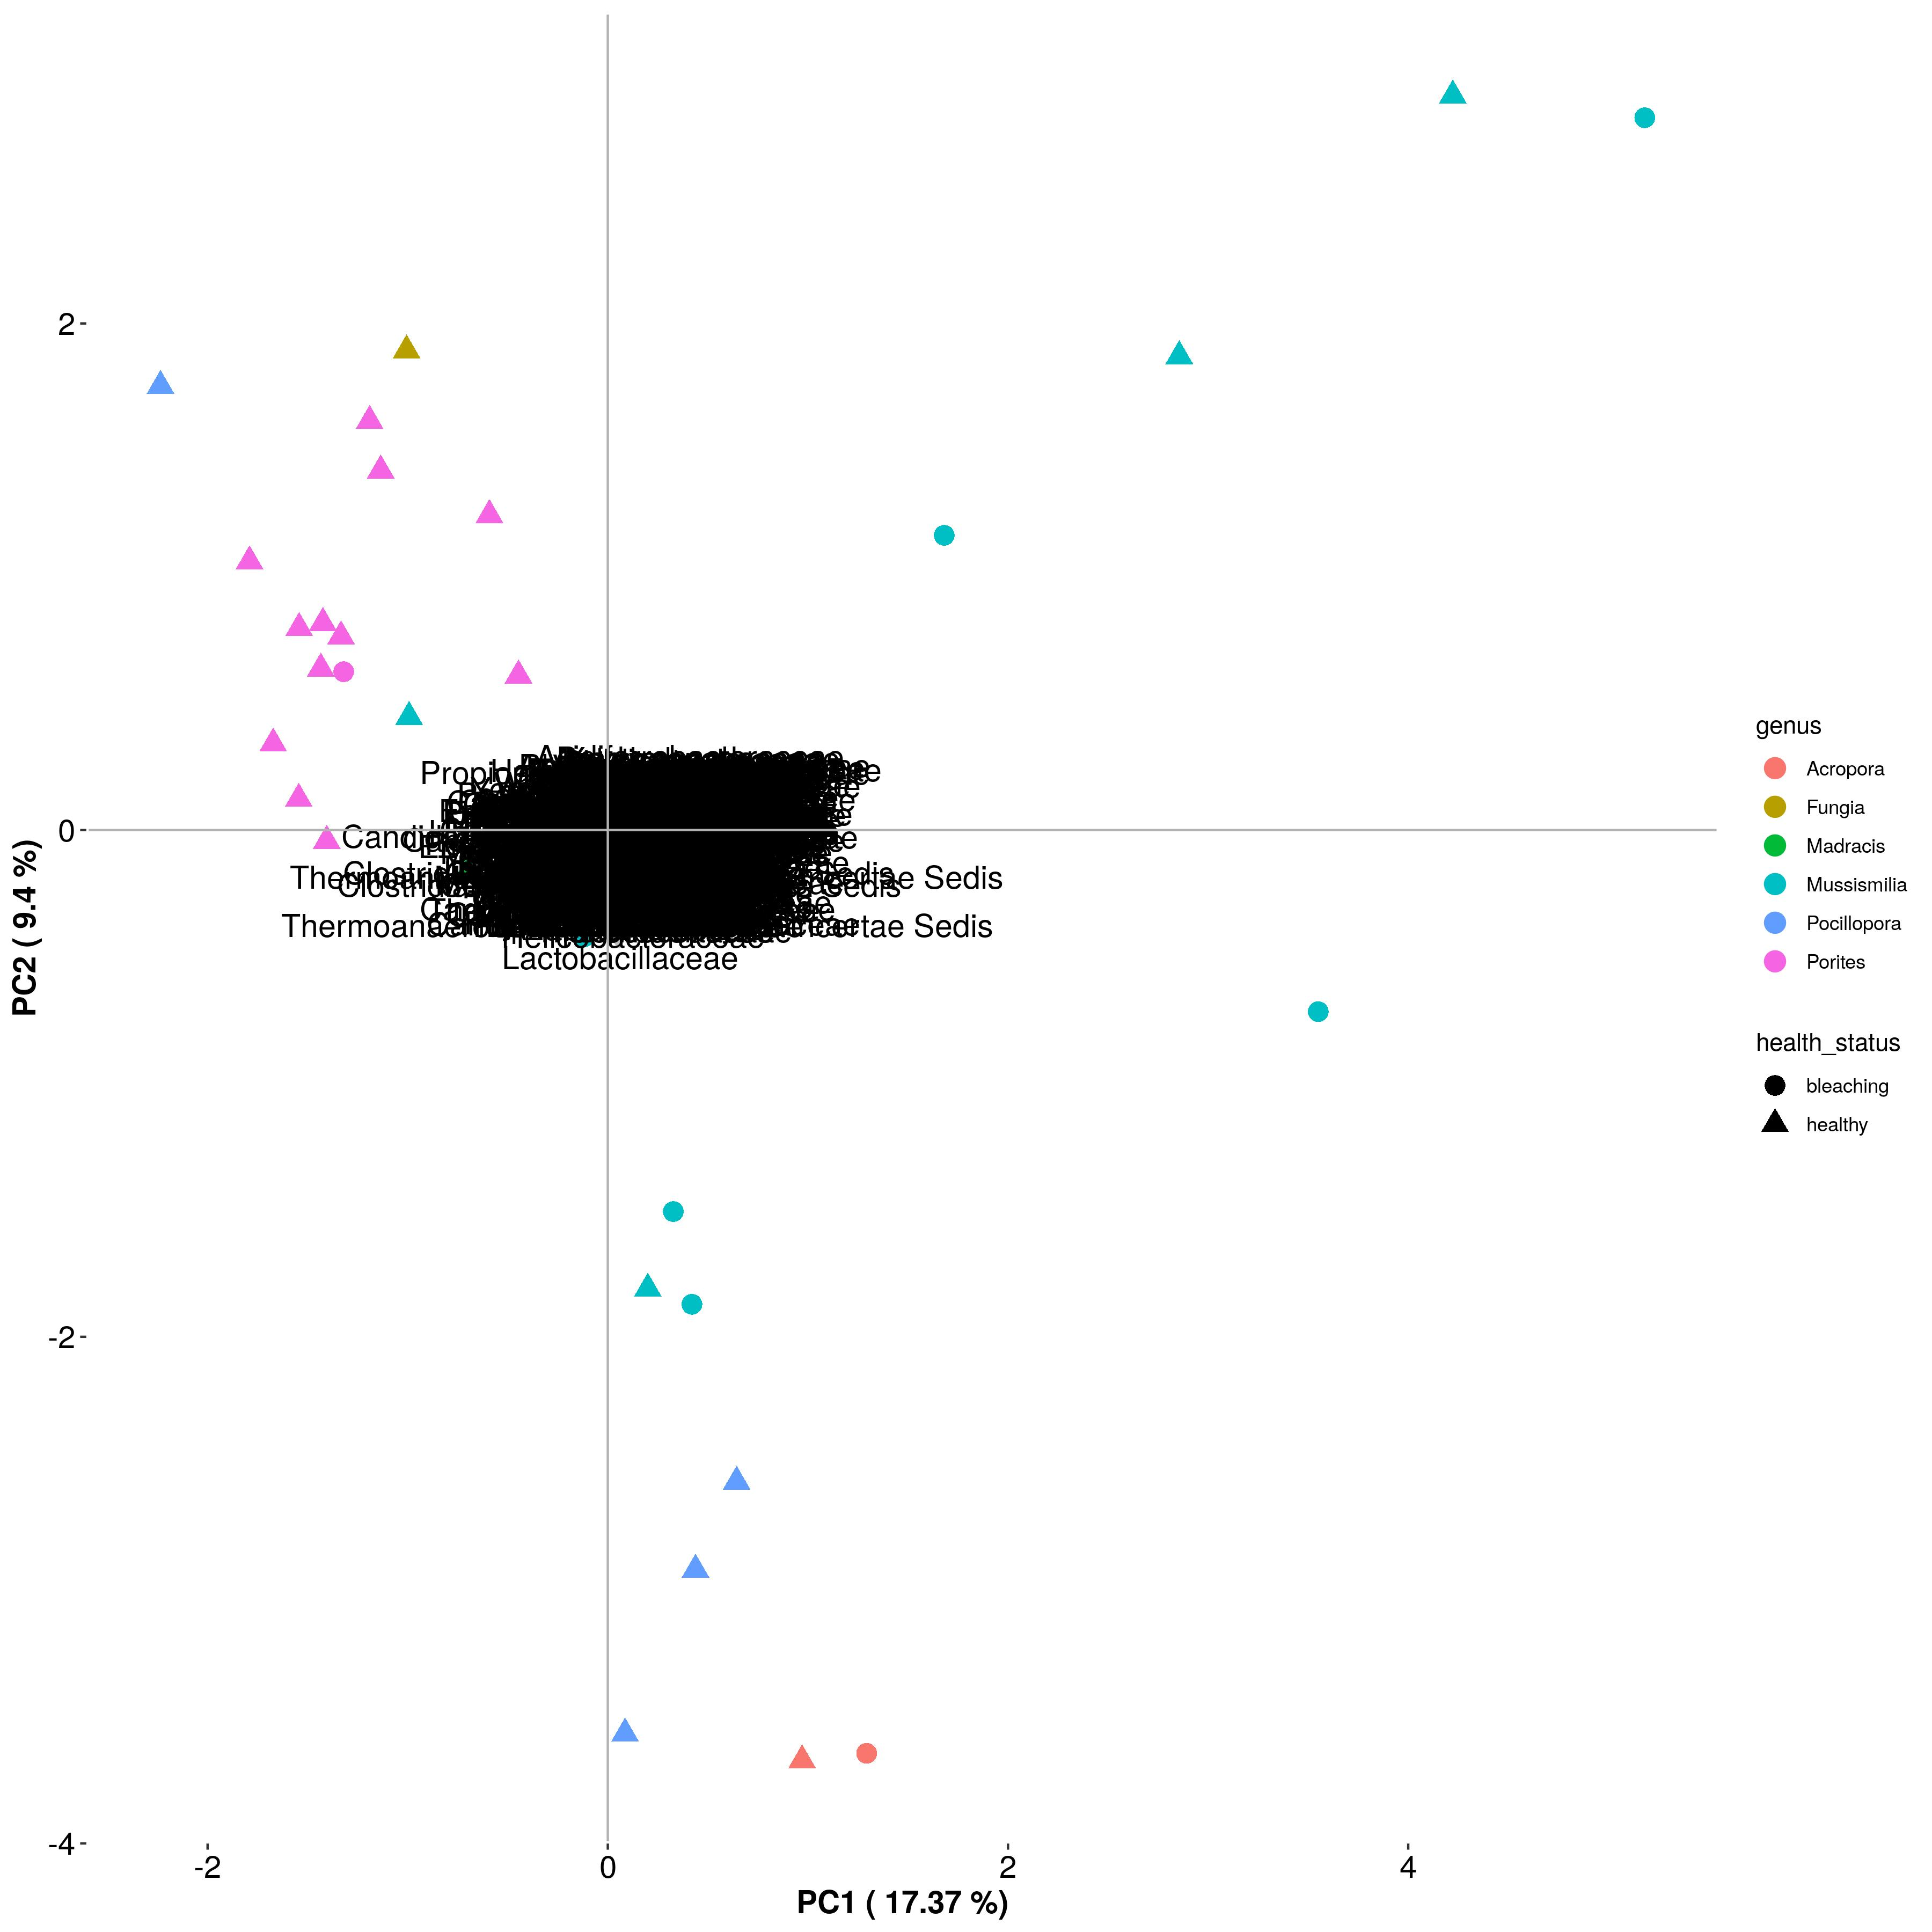
\includegraphics[scale=0.4]{figures/familia/output_PCA_corais_familia_mg_rast_2018_10_30.jpg}
\caption{PCA geral feito com matriz de abundancia de familias}
\label{fig:PCAfeito30deoutubroparafamilia}
\end{figure}

\begin{figure}[H]
\centering
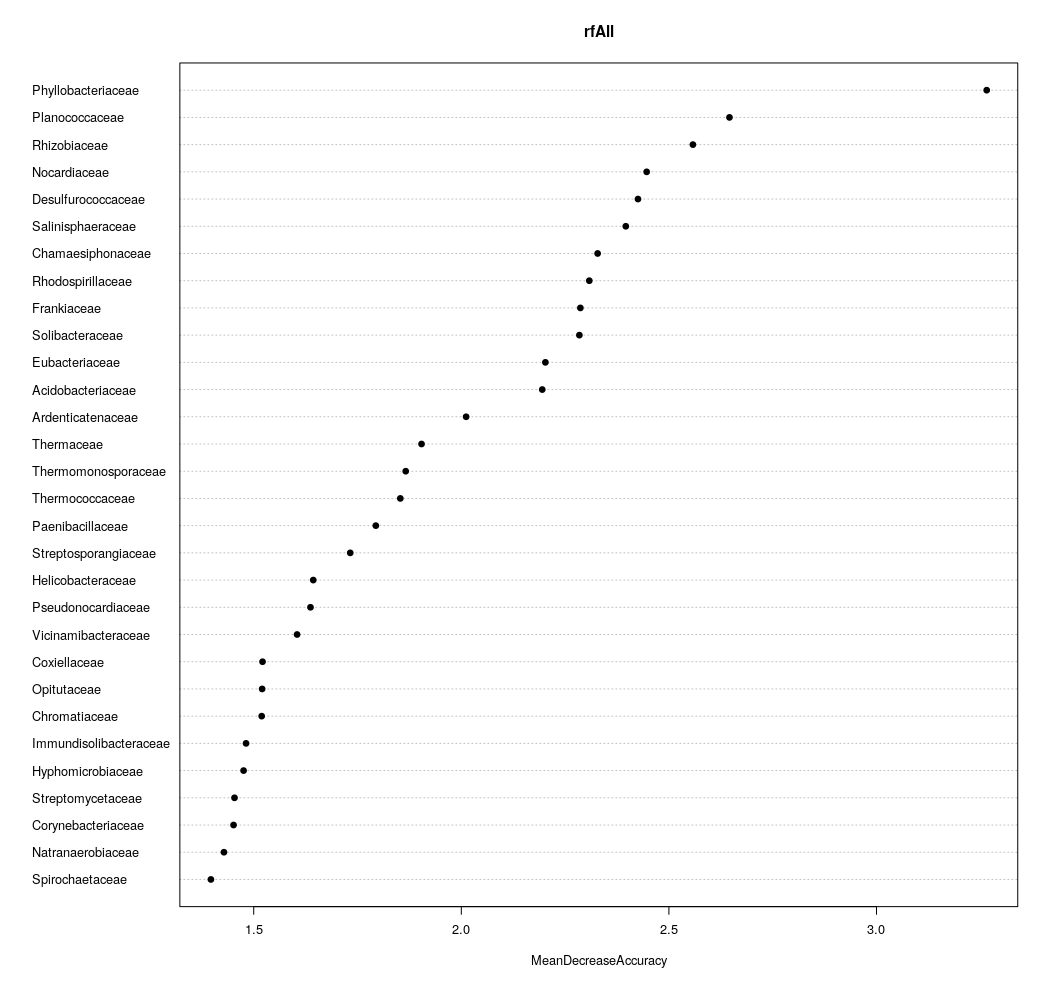
\includegraphics[scale=0.4]{figures/familia/randomforest_nao_supervi_corais_mgrast_familia_leticia_2018_10_30.jpeg}
\caption{RANDOM FOREST NAO SUPERVISIONADO PARA FAMILIAS}
\label{fig:Randomforestnaosupervisionadoparafamilafeito30deoutubroparafamilia}
\end{figure}

\begin{figure}[H]
\centering
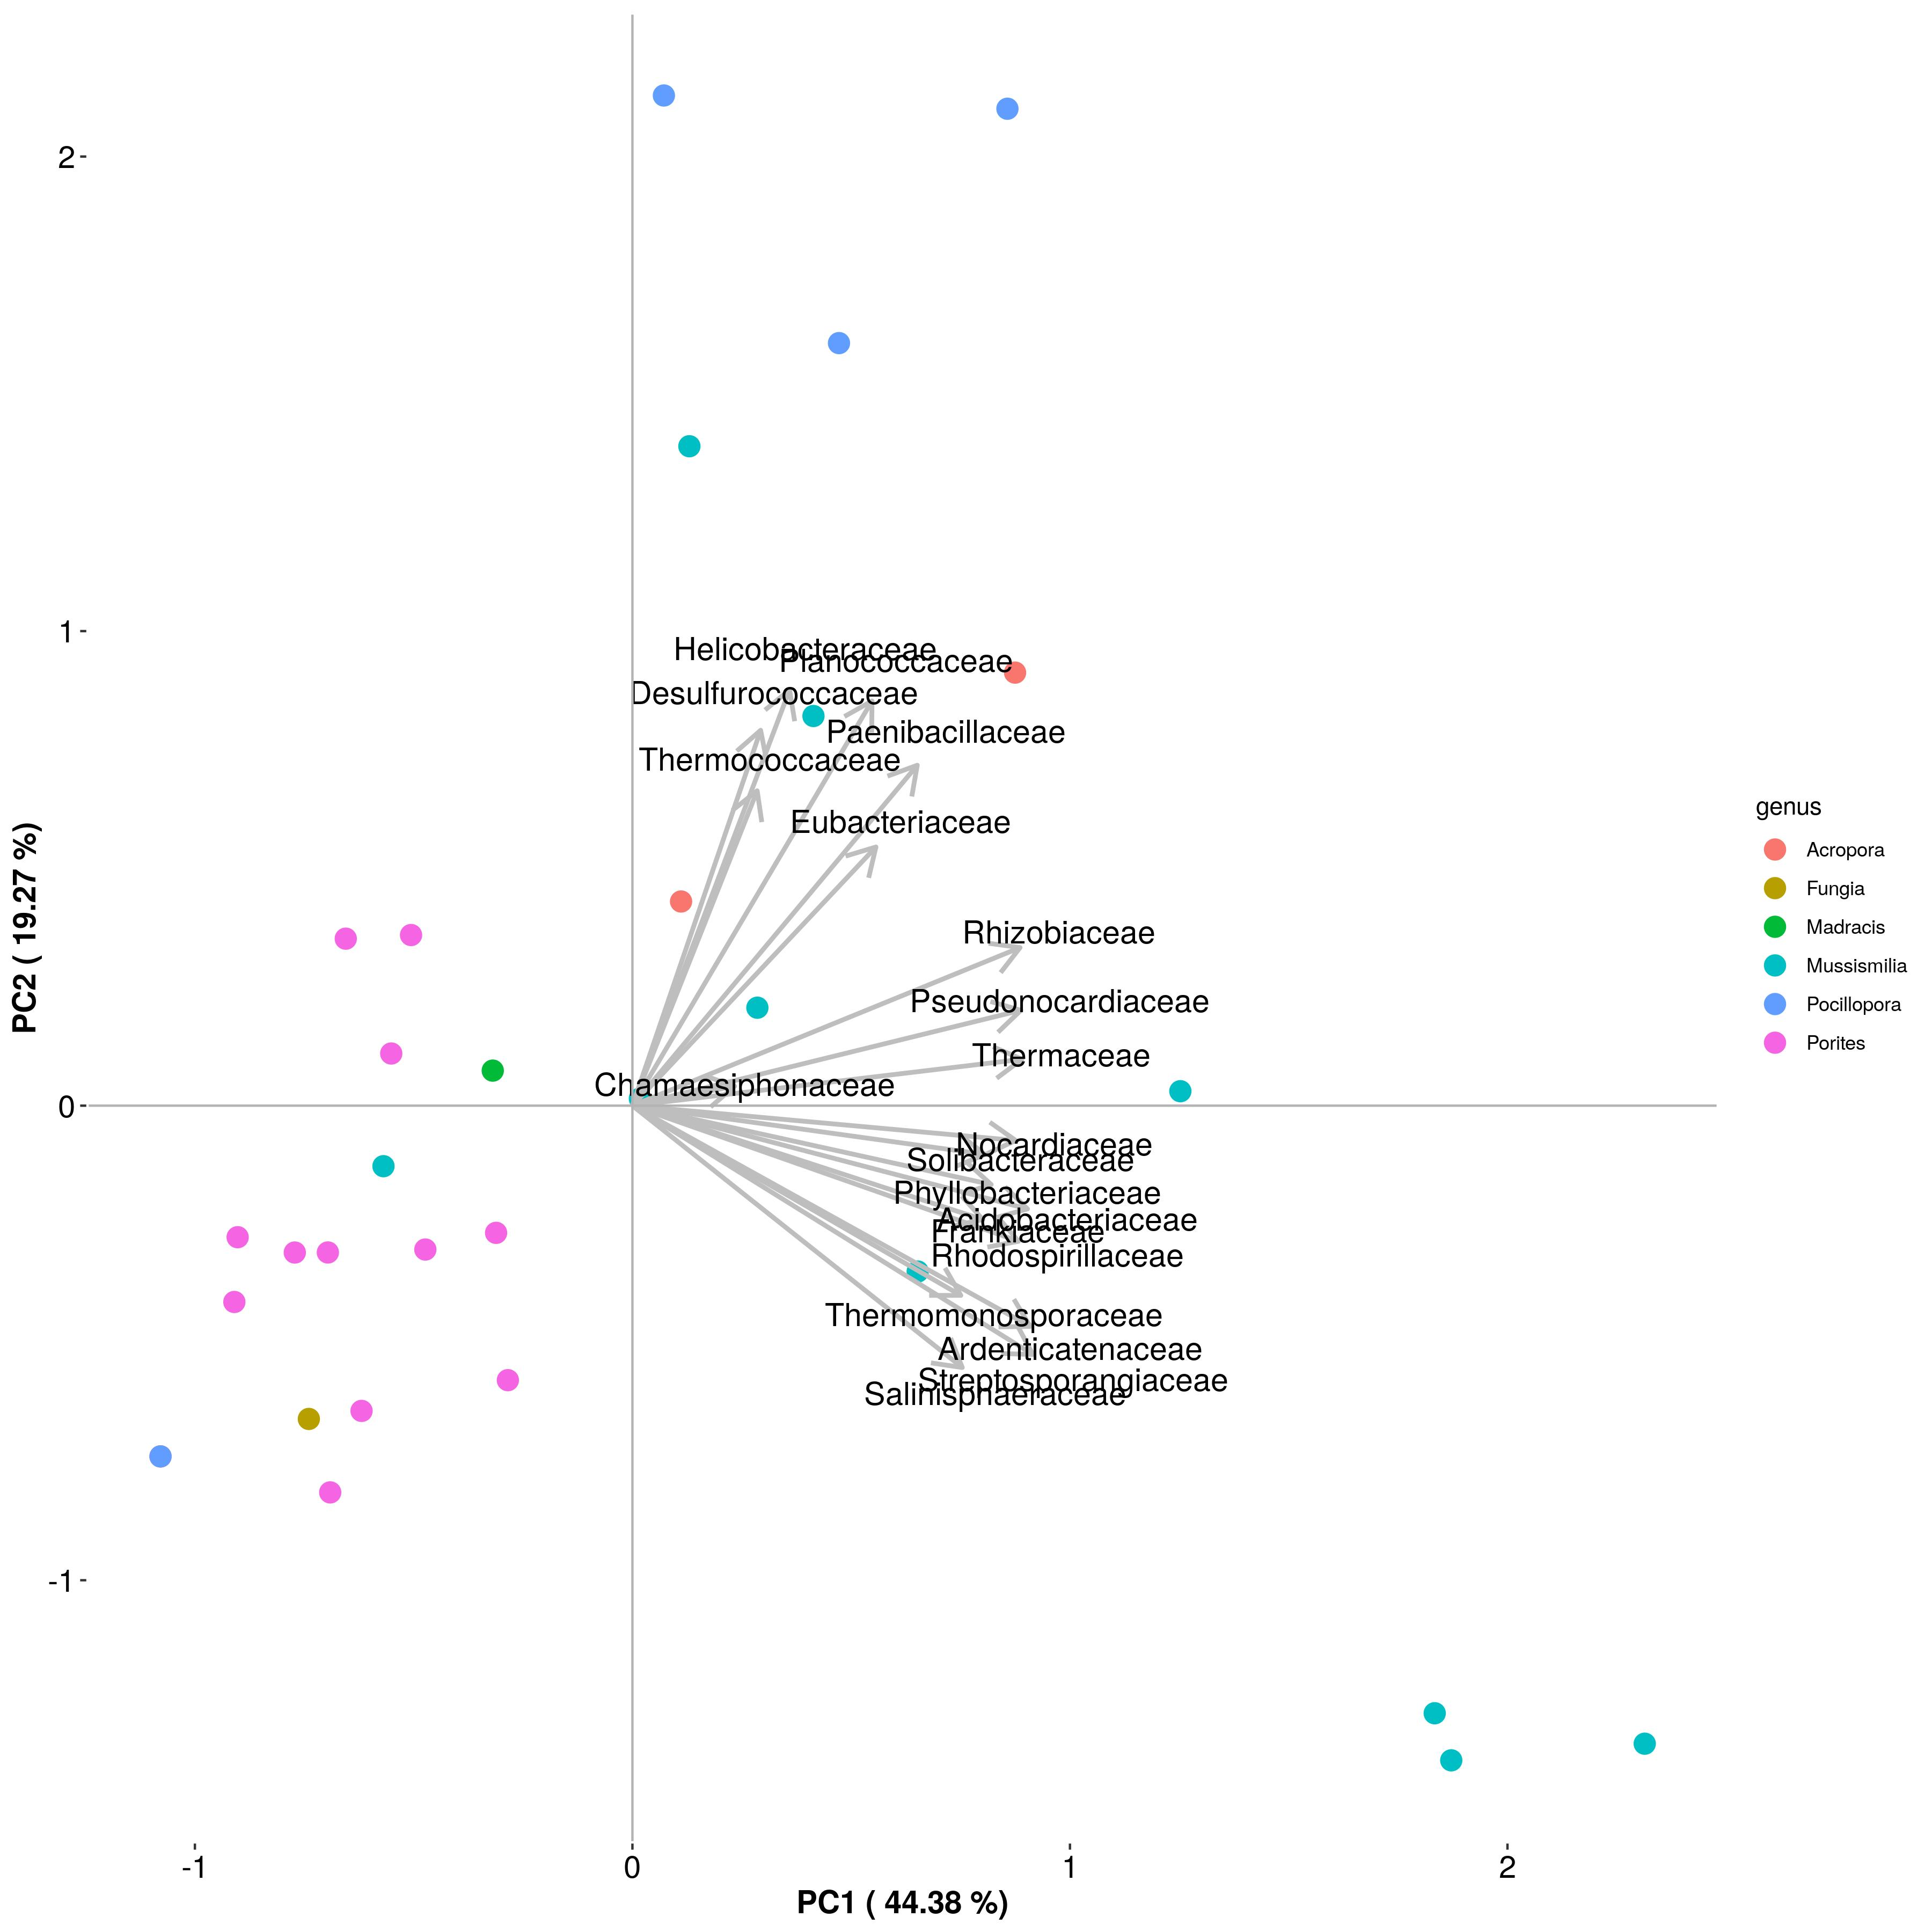
\includegraphics[scale=0.3]{figures/familia/pca_corais_mgrast_rf_nao_supervisionado_20_familias_30_10_2018.jpg}
\caption{PCA FEITO COM OS 20 FAMILIAS INDICADOS PELO RANDOM FOREST NÃO SUPERVISIONADO PARA FAMILIAS}
\label{fig:PCAFEITOCOM20FAMILIAS}
\end{figure}

\begin{figure}[H]
\centering
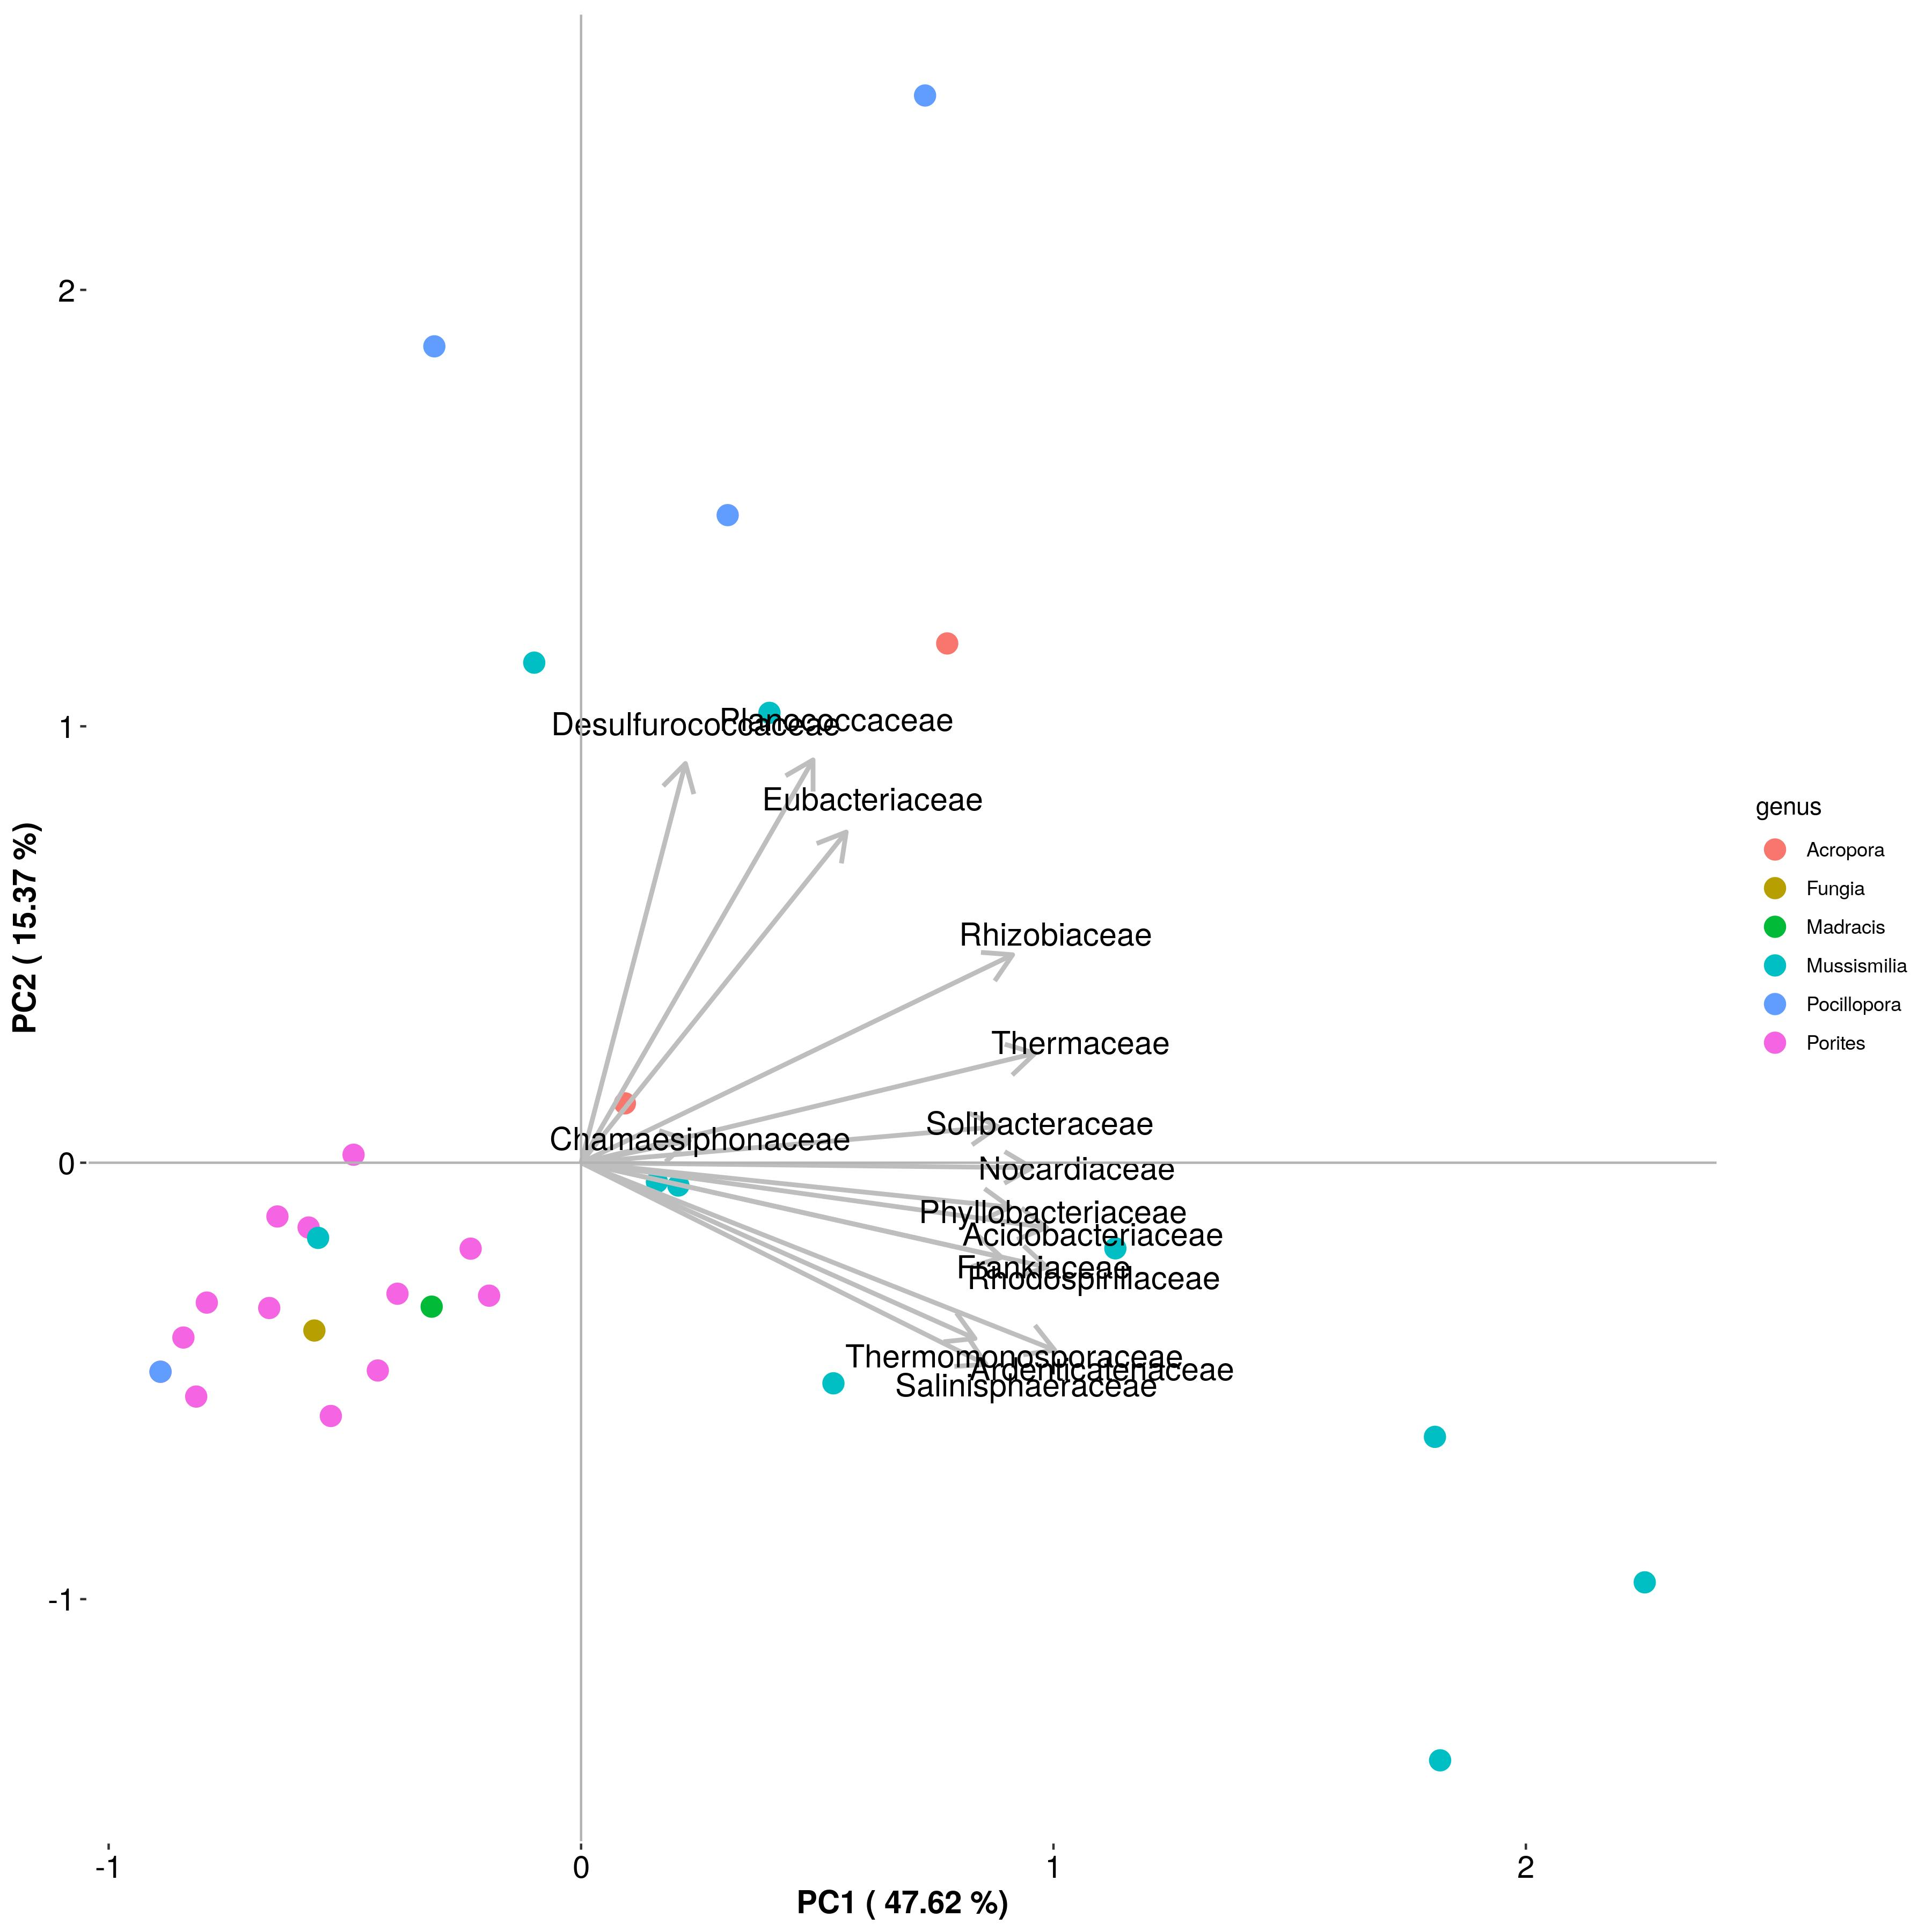
\includegraphics[scale=0.3]{figures/familia/pca_corais_mgrast_rf_nao_supervisionado_15_familias_30_10_2018.jpg}
\caption{PCA FEITO COM OS 15 FAMILIAS INDICADOS PELO RANDOM FOREST NÃO SUPERVISIONADO PARA FAMILIAS}
\label{fig:PCAFEITOCOM15FAMILIAS}
\end{figure}


\begin{figure}[H]
\centering
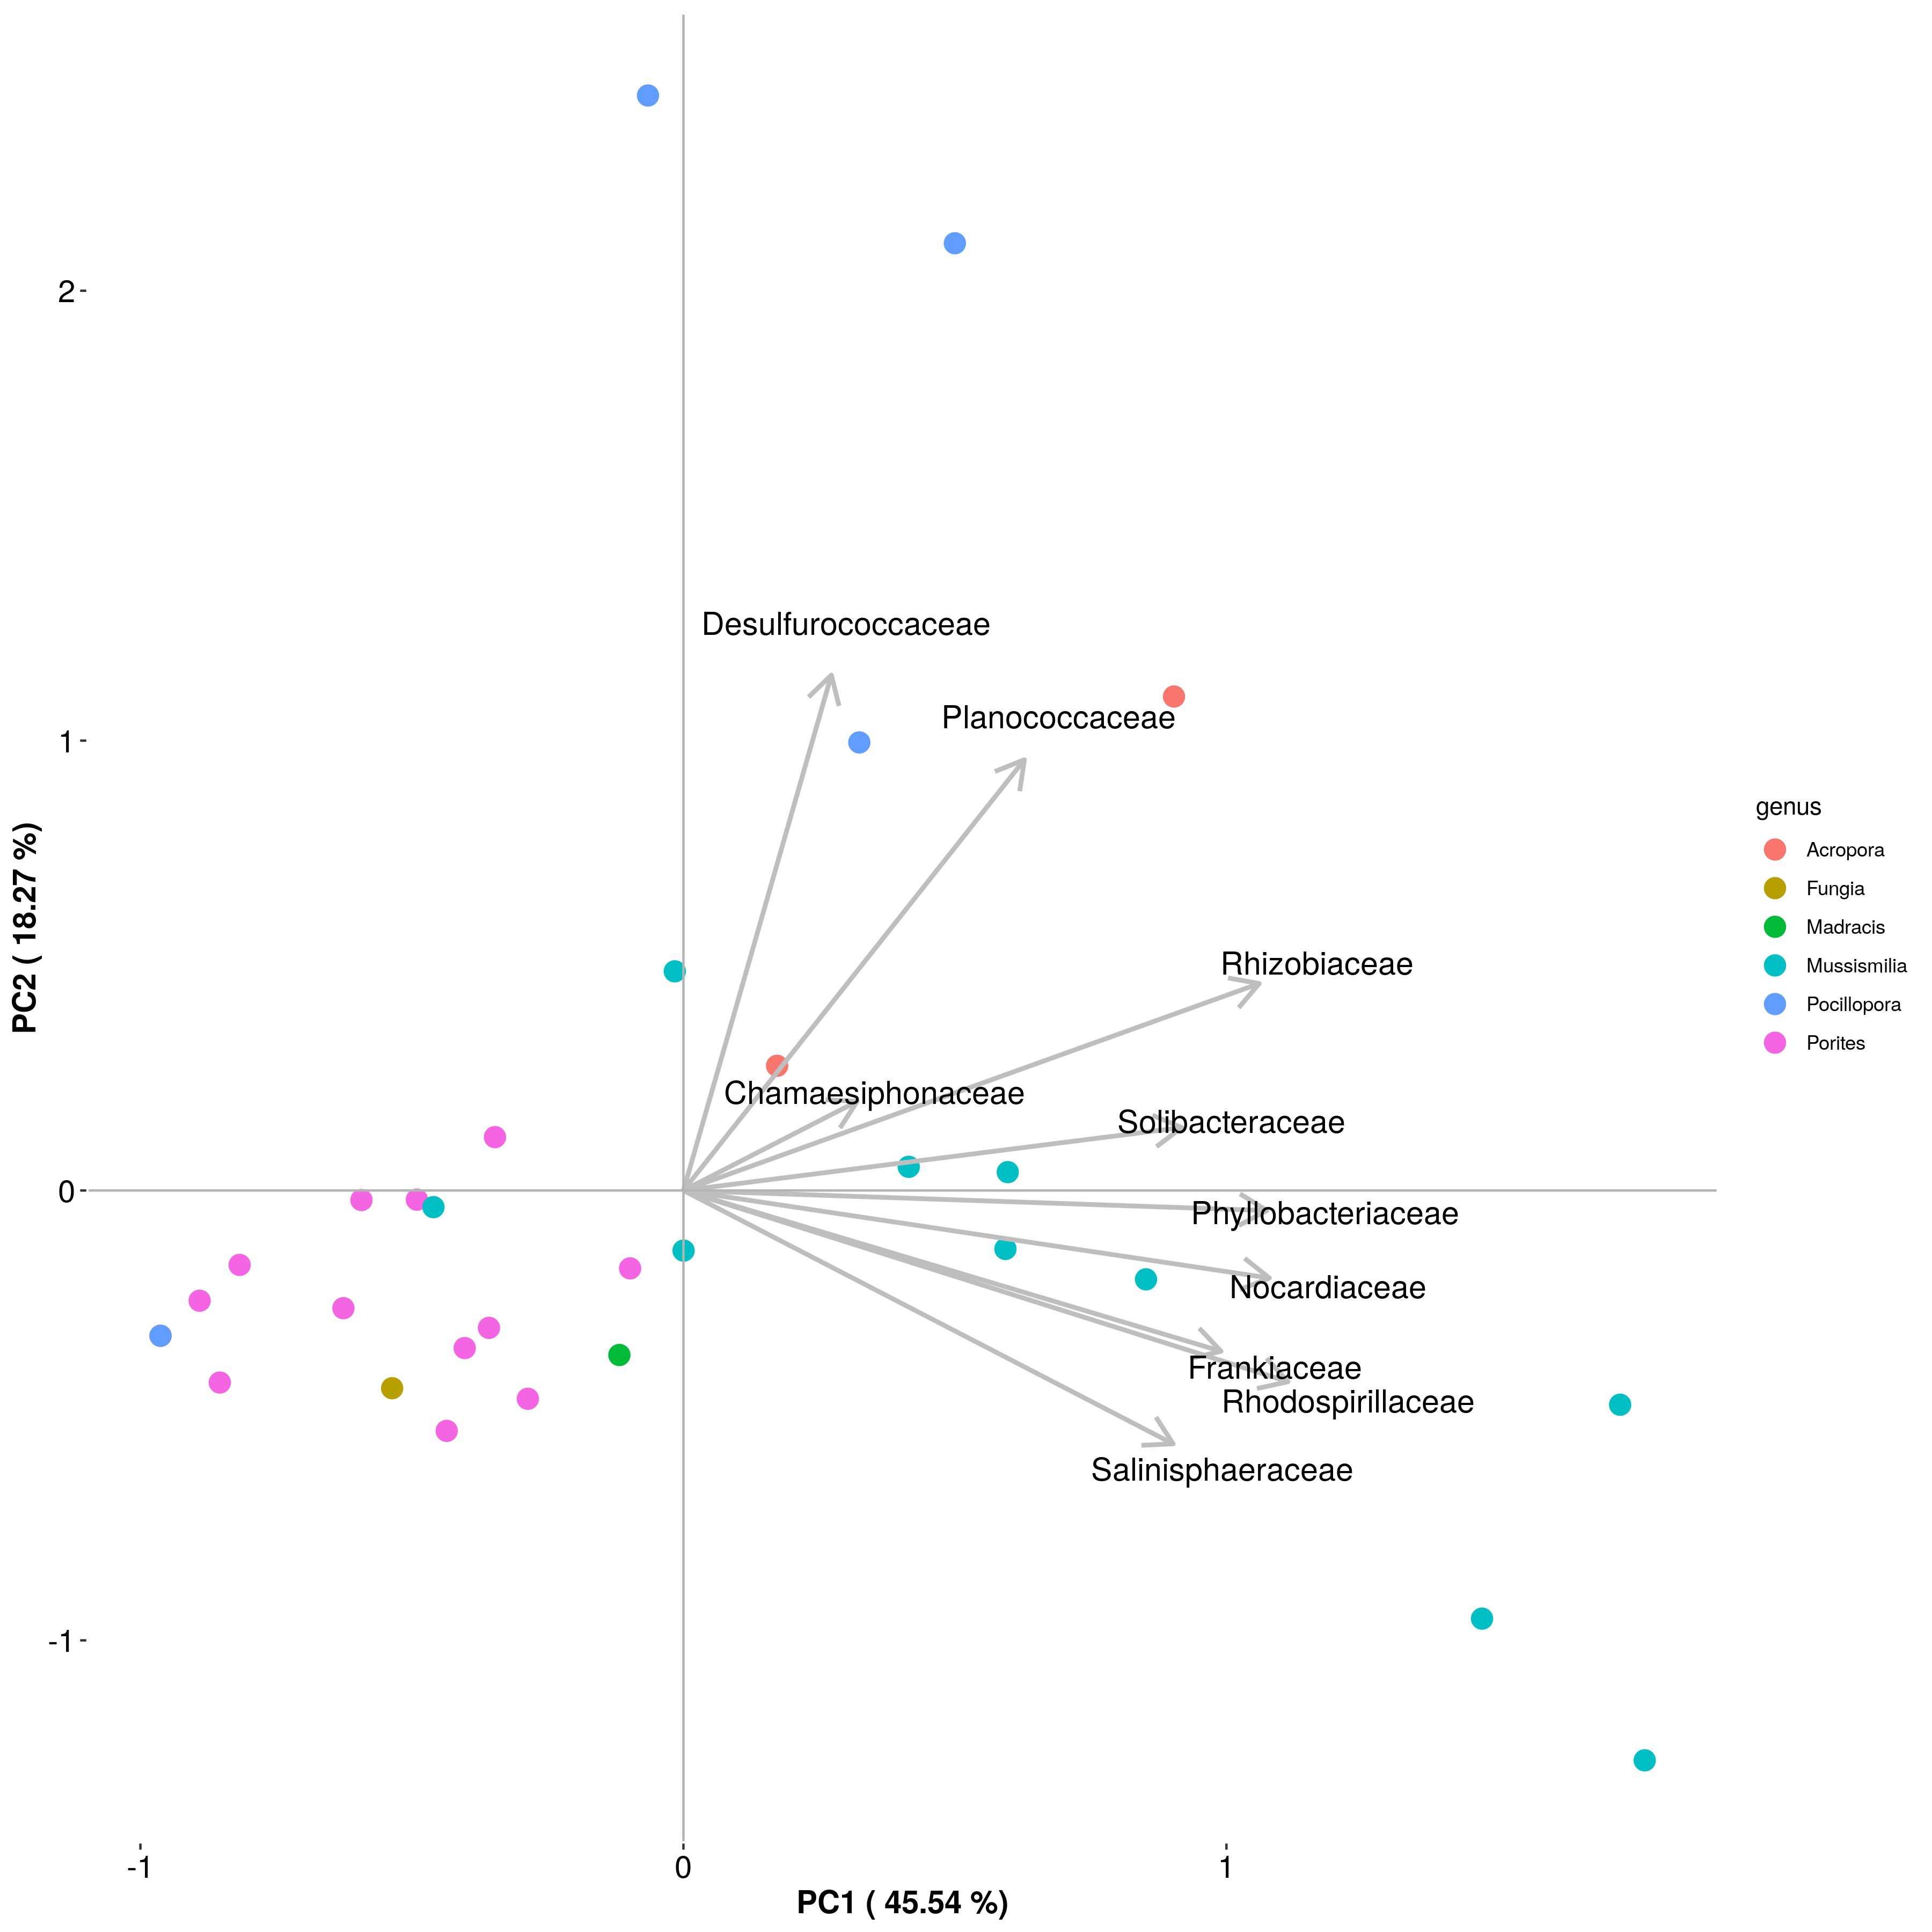
\includegraphics[scale=0.3]{figures/familia/pca_corais_mgrast_rf_nao_supervisionado_10_familias_30_10_2018.jpg}
\caption{PCA FEITO COM OS 10 FAMILIAS INDICADOS PELO RANDOM FOREST NÃO SUPERVISIONADO PARA FAMILIAS}
\label{fig:PCAFEITOCOM10FAMILIAS}
\end{figure}

\begin{figure}[H]
\centering
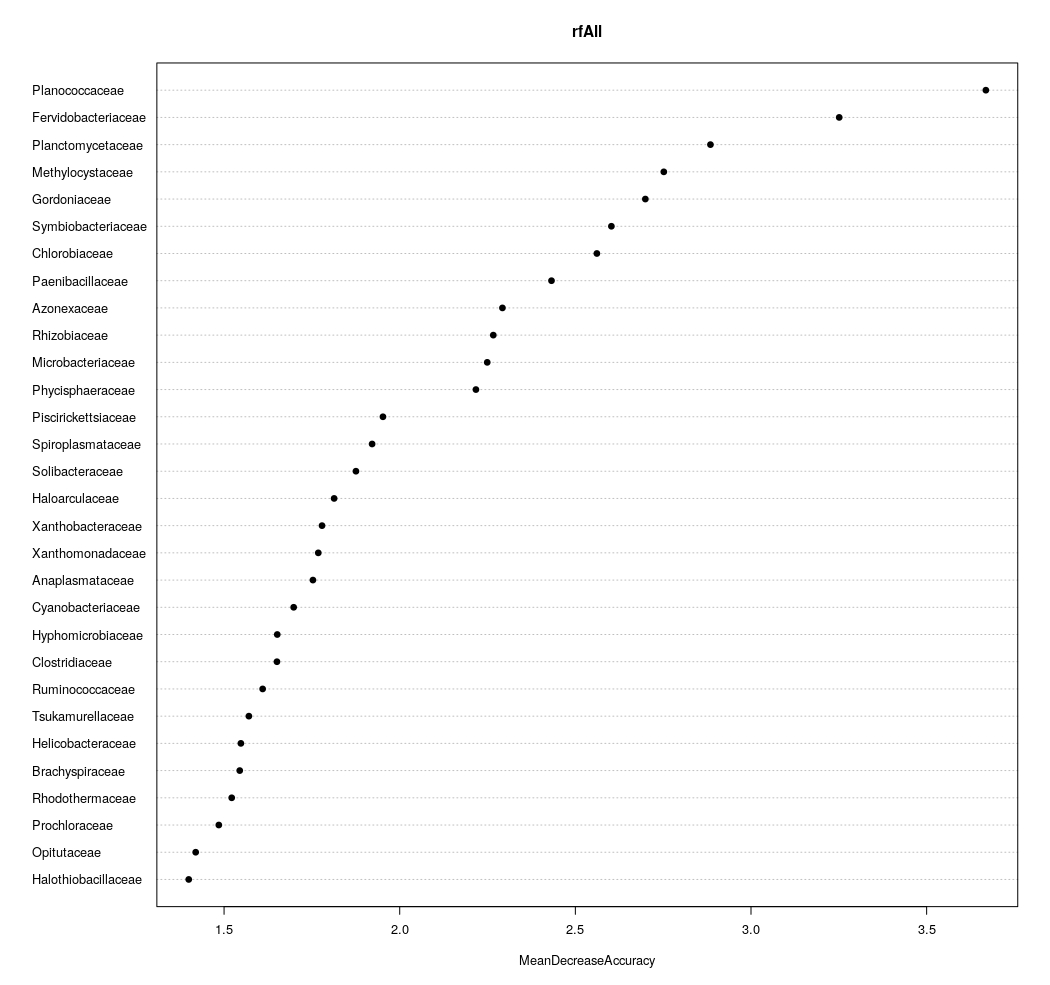
\includegraphics[scale=0.3]{figures/familia/randomforest_supervisionado_genero_corais_mgrast_familia_leticia_2018_10_30.jpeg}
\caption{RANDOM FOREST SUPERVISIONADO POR GENERO}
\label{fig:RFSUPERVISIONADOGENEROPFAMILIAS}
\end{figure}

\begin{figure}[H]
\centering
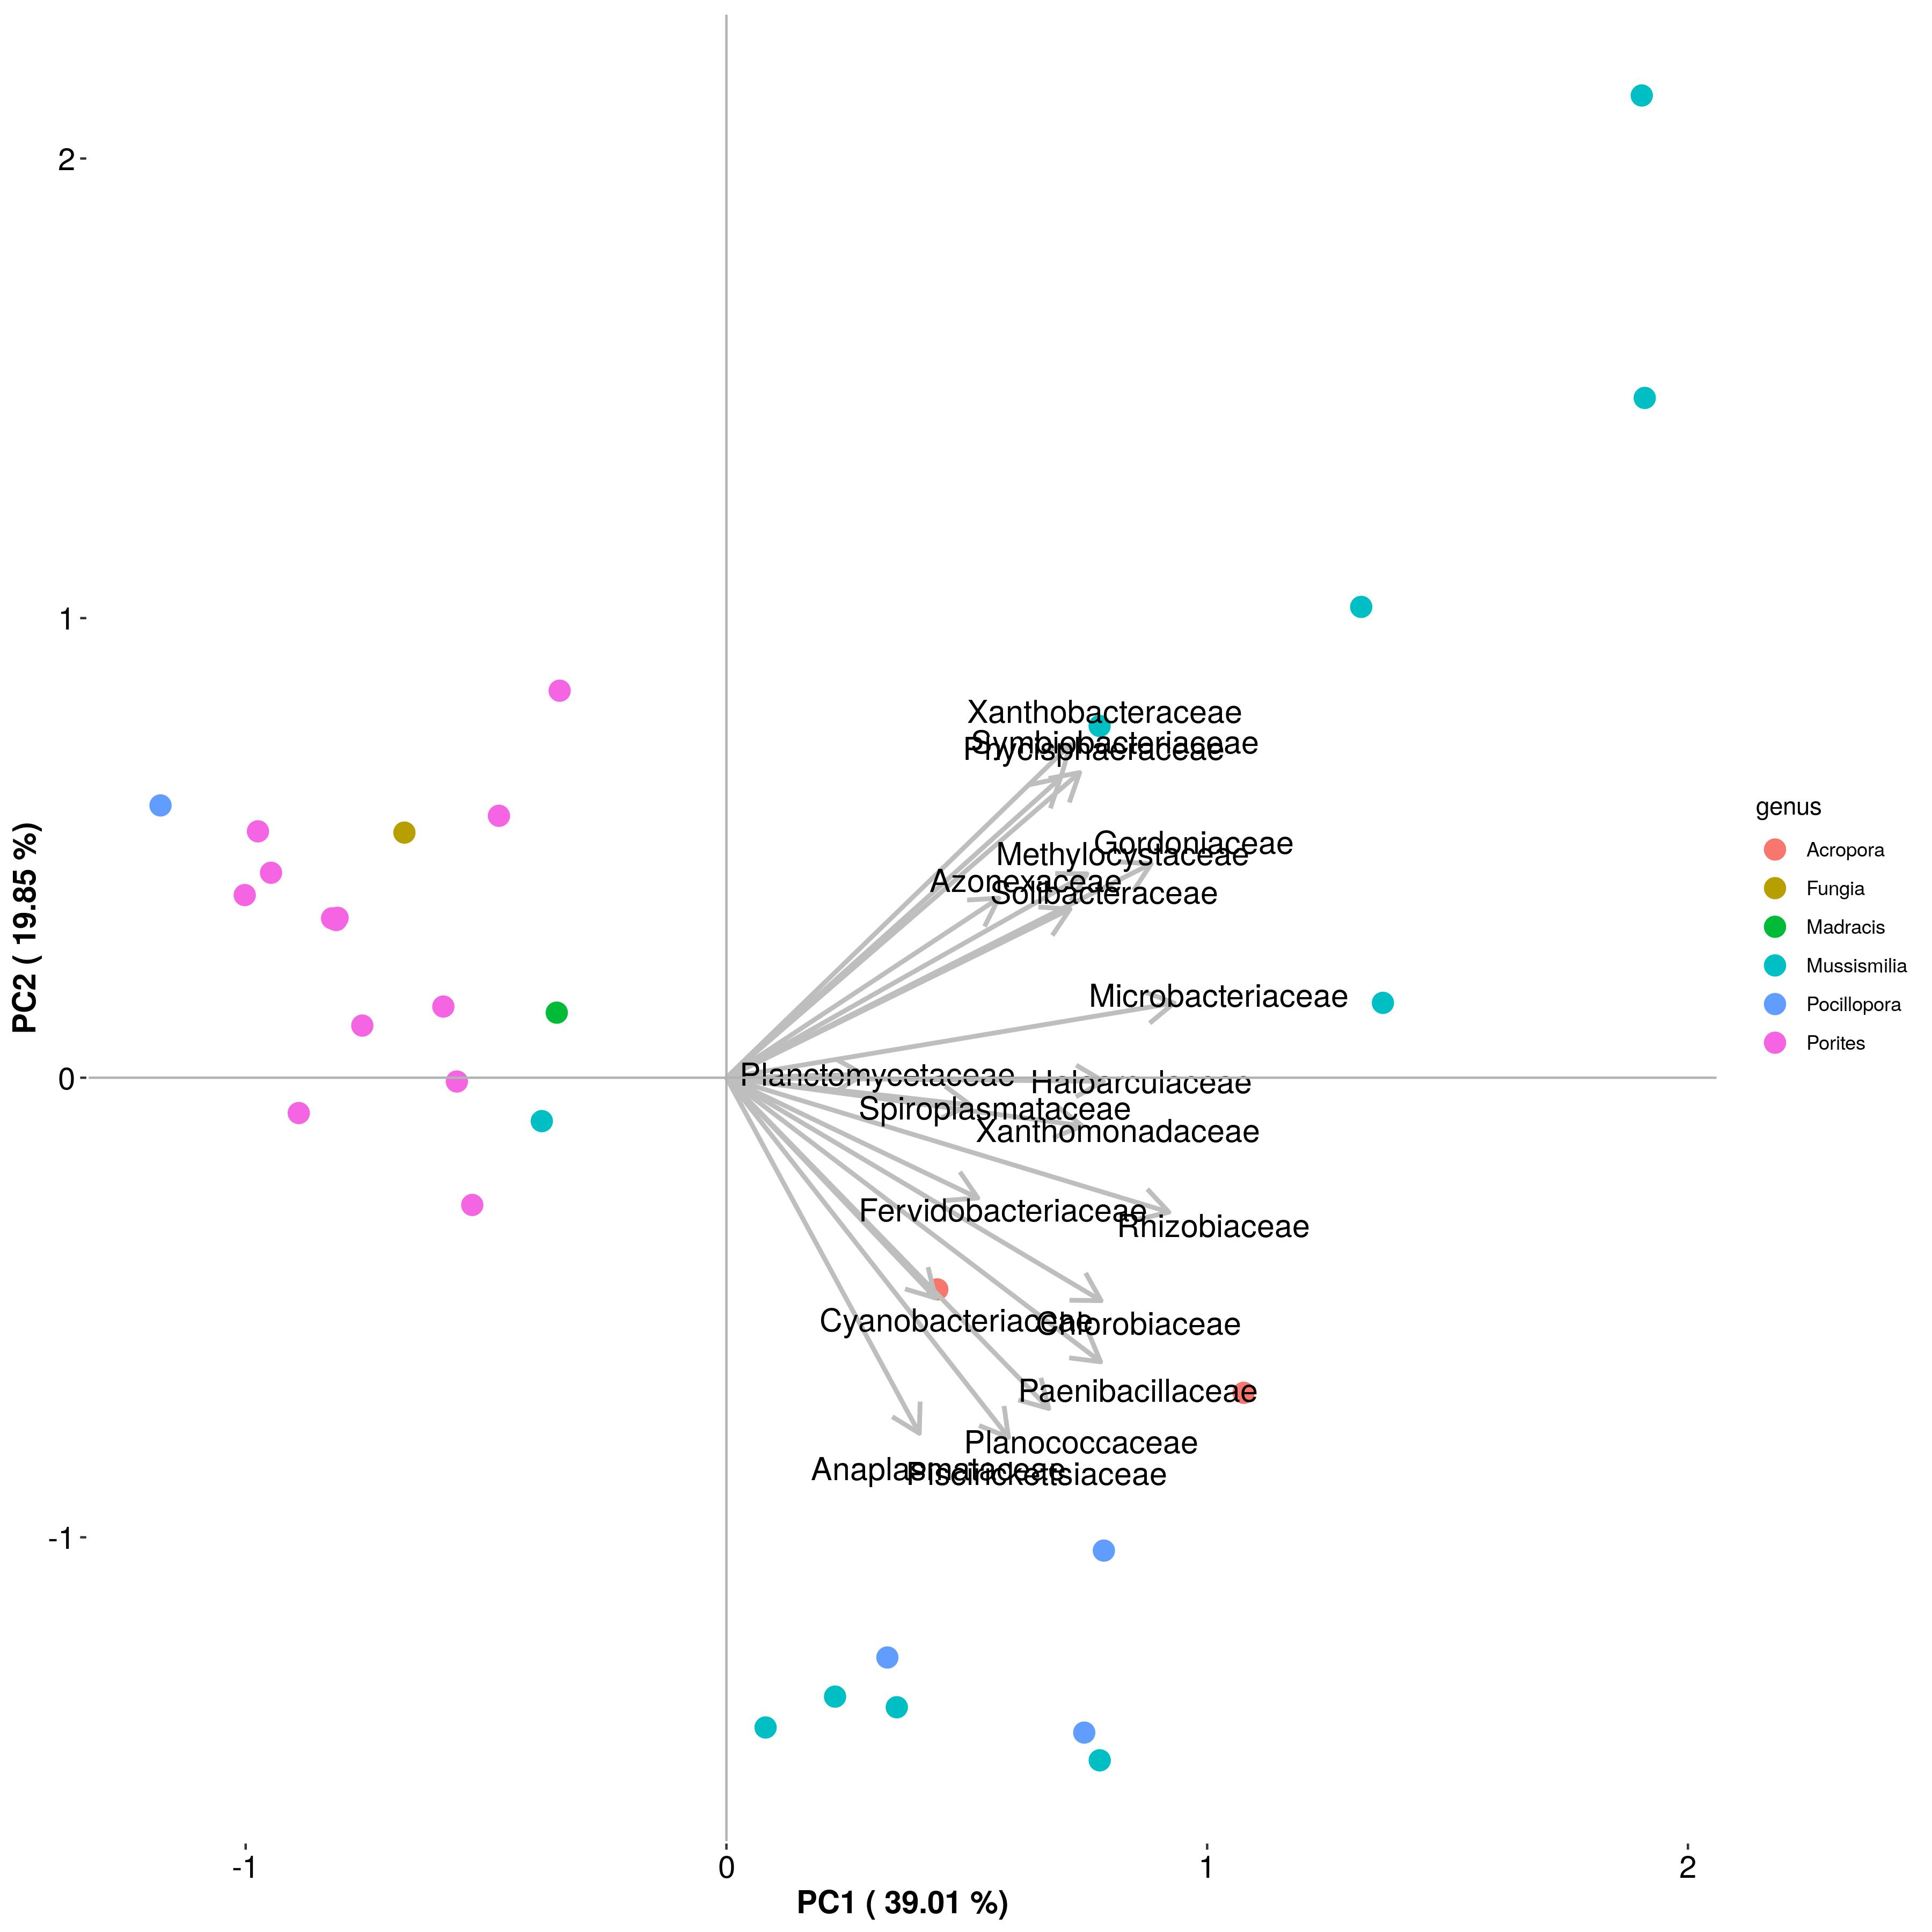
\includegraphics[scale=0.3]{figures/familia/pca_corais_mg_rast_rf_supervisionado_genus_20_familias_23_10_2018.jpg}
\caption{PCA FEITO COM OS 20 FAMILIAS INDICADOS PELO RANDOM FOREST SUPERVISIONADO POR GENERO PARA FAMILIAS DE MICRORGANISMOS}
\label{fig:PCA20FAMILIASDERIVADODORFSUPERVISIONADOGENEROPFAMILIAS}
\end{figure}

\begin{figure}[H]
\centering
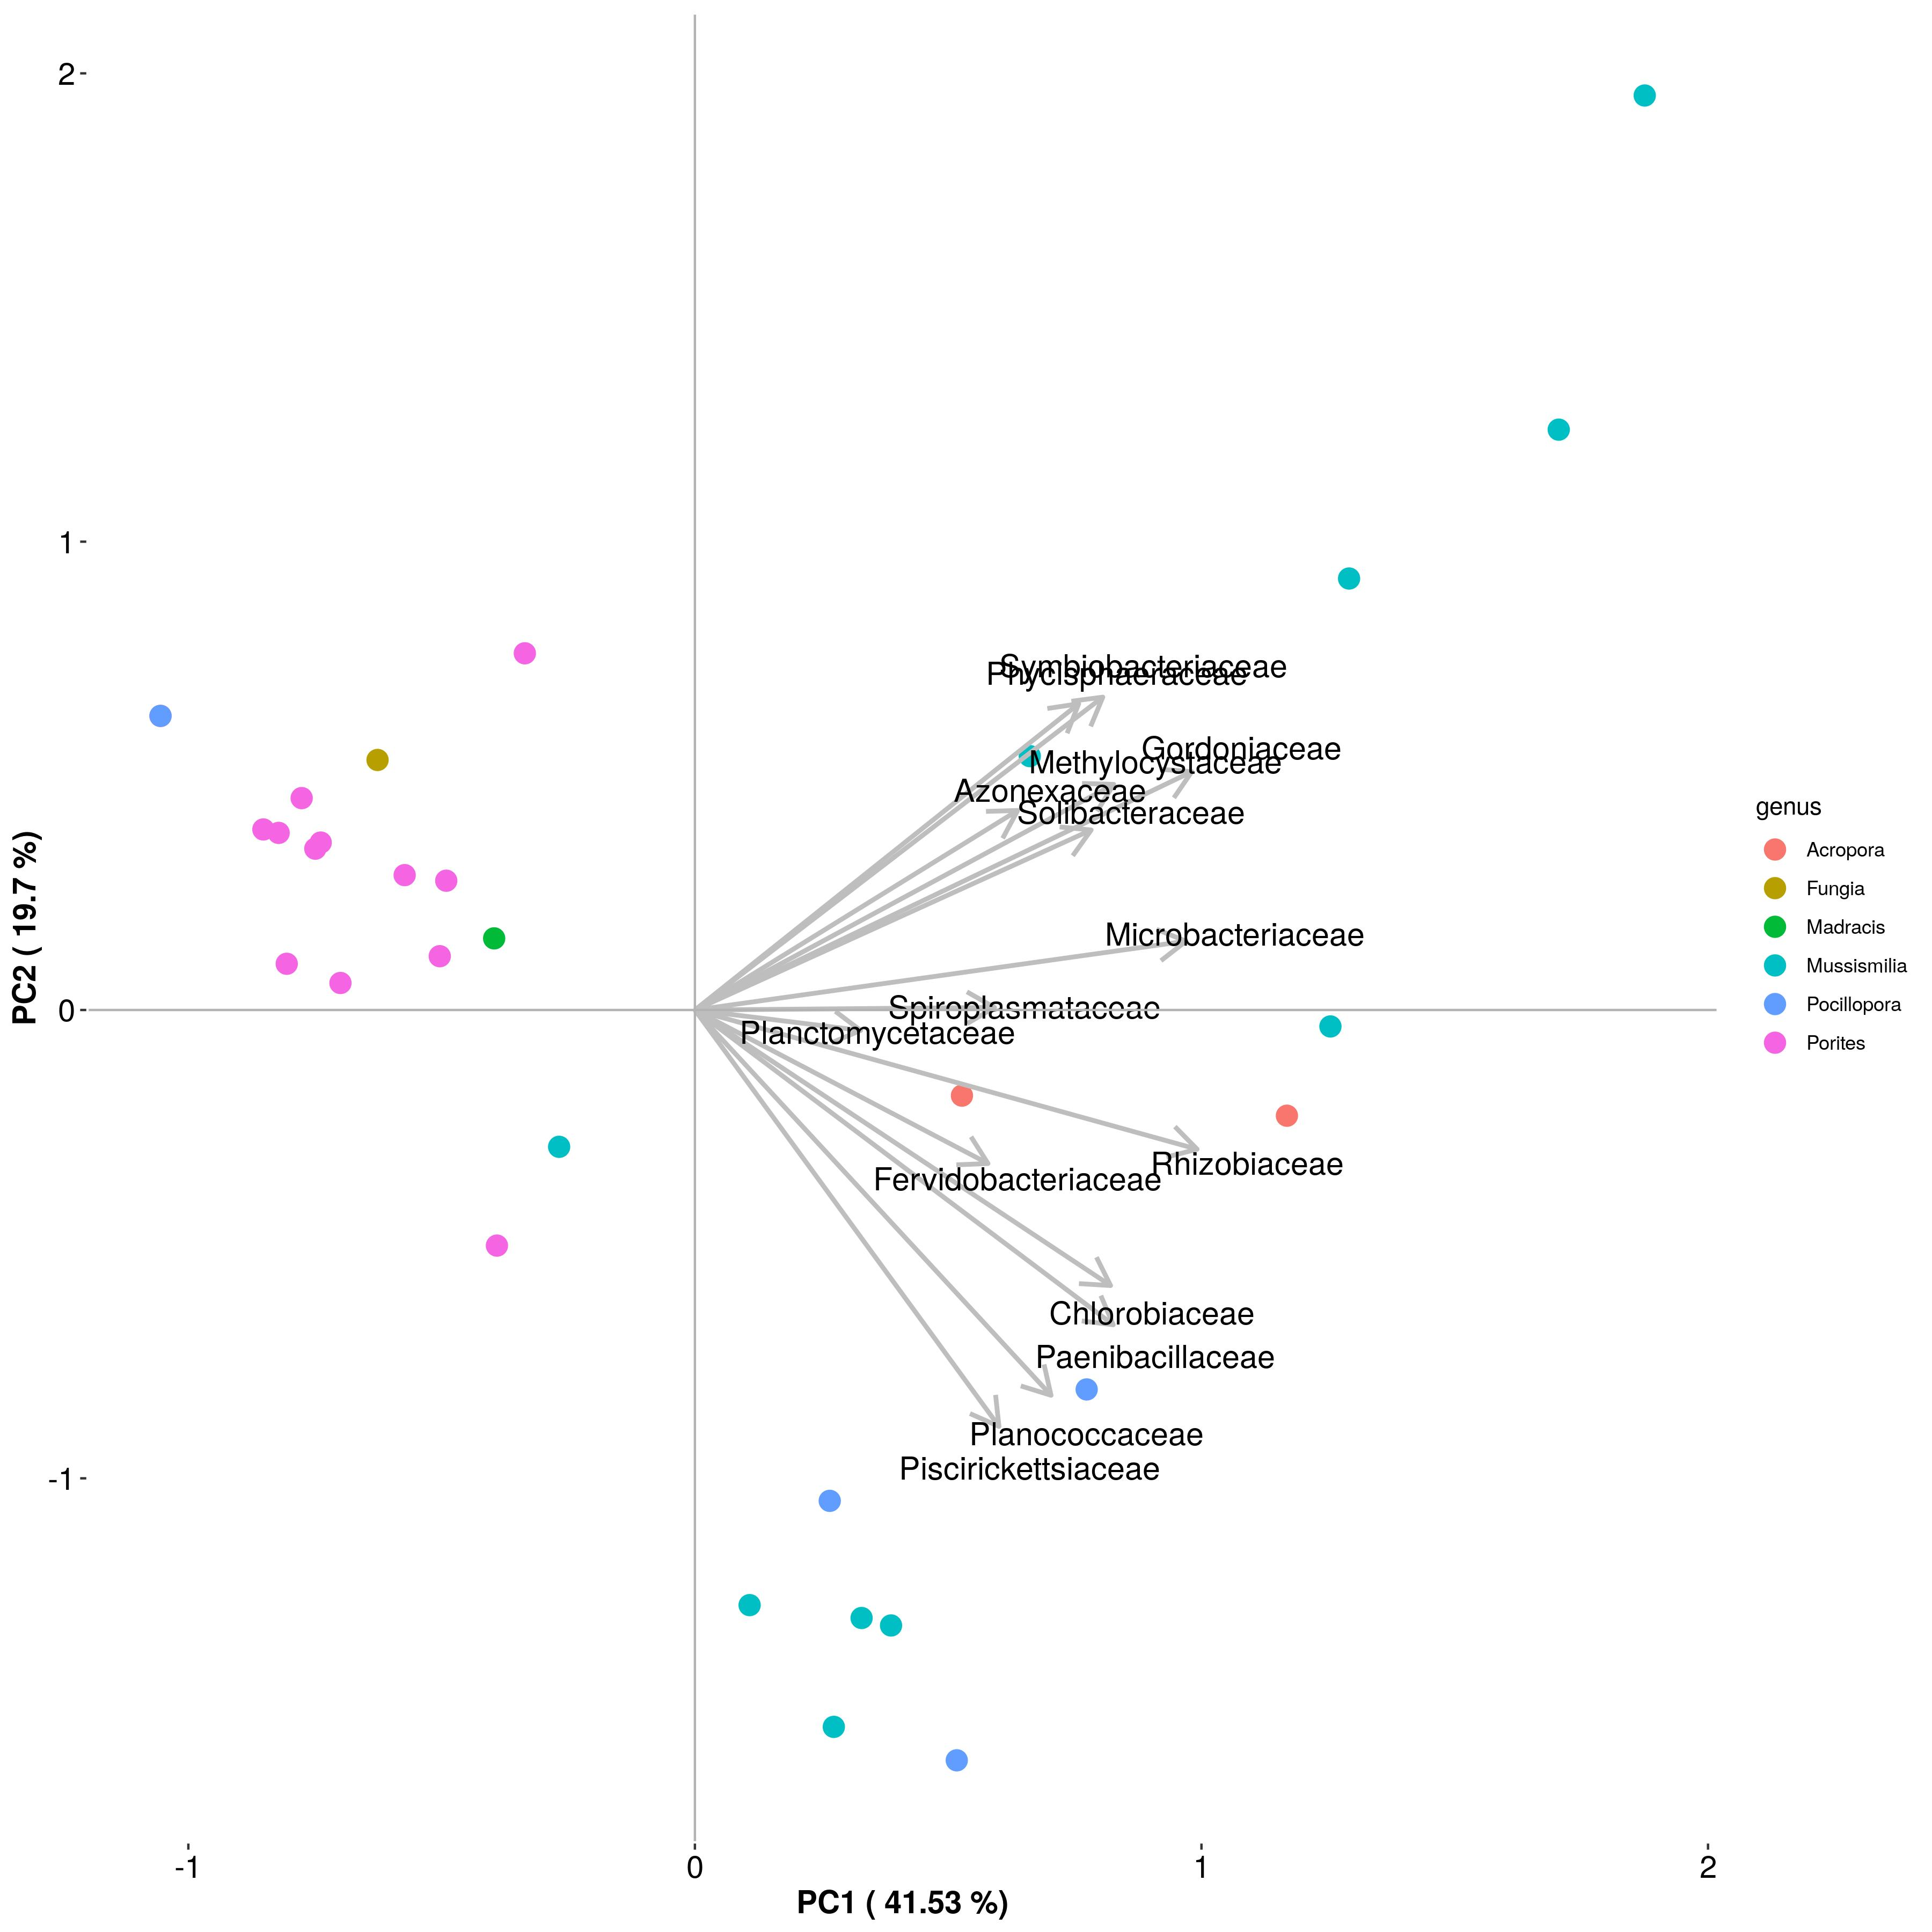
\includegraphics[scale=0.3]{figures/familia/pca_corais_mg_rast_rf_supervisionado_genus_15_familias_30_10_2018.jpg}
\caption{PCA FEITO COM OS 15 FAMILIAS INDICADOS PELO RANDOM FOREST SUPERVISIONADO POR GENERO PARA FAMILIAS DE MICRORGANISMOS}
\label{fig:PCA15FAMILIASDERIVADODORFSUPERVISIONADOGENEROPFAMILIAS}
\end{figure}

\begin{figure}[H]
\centering
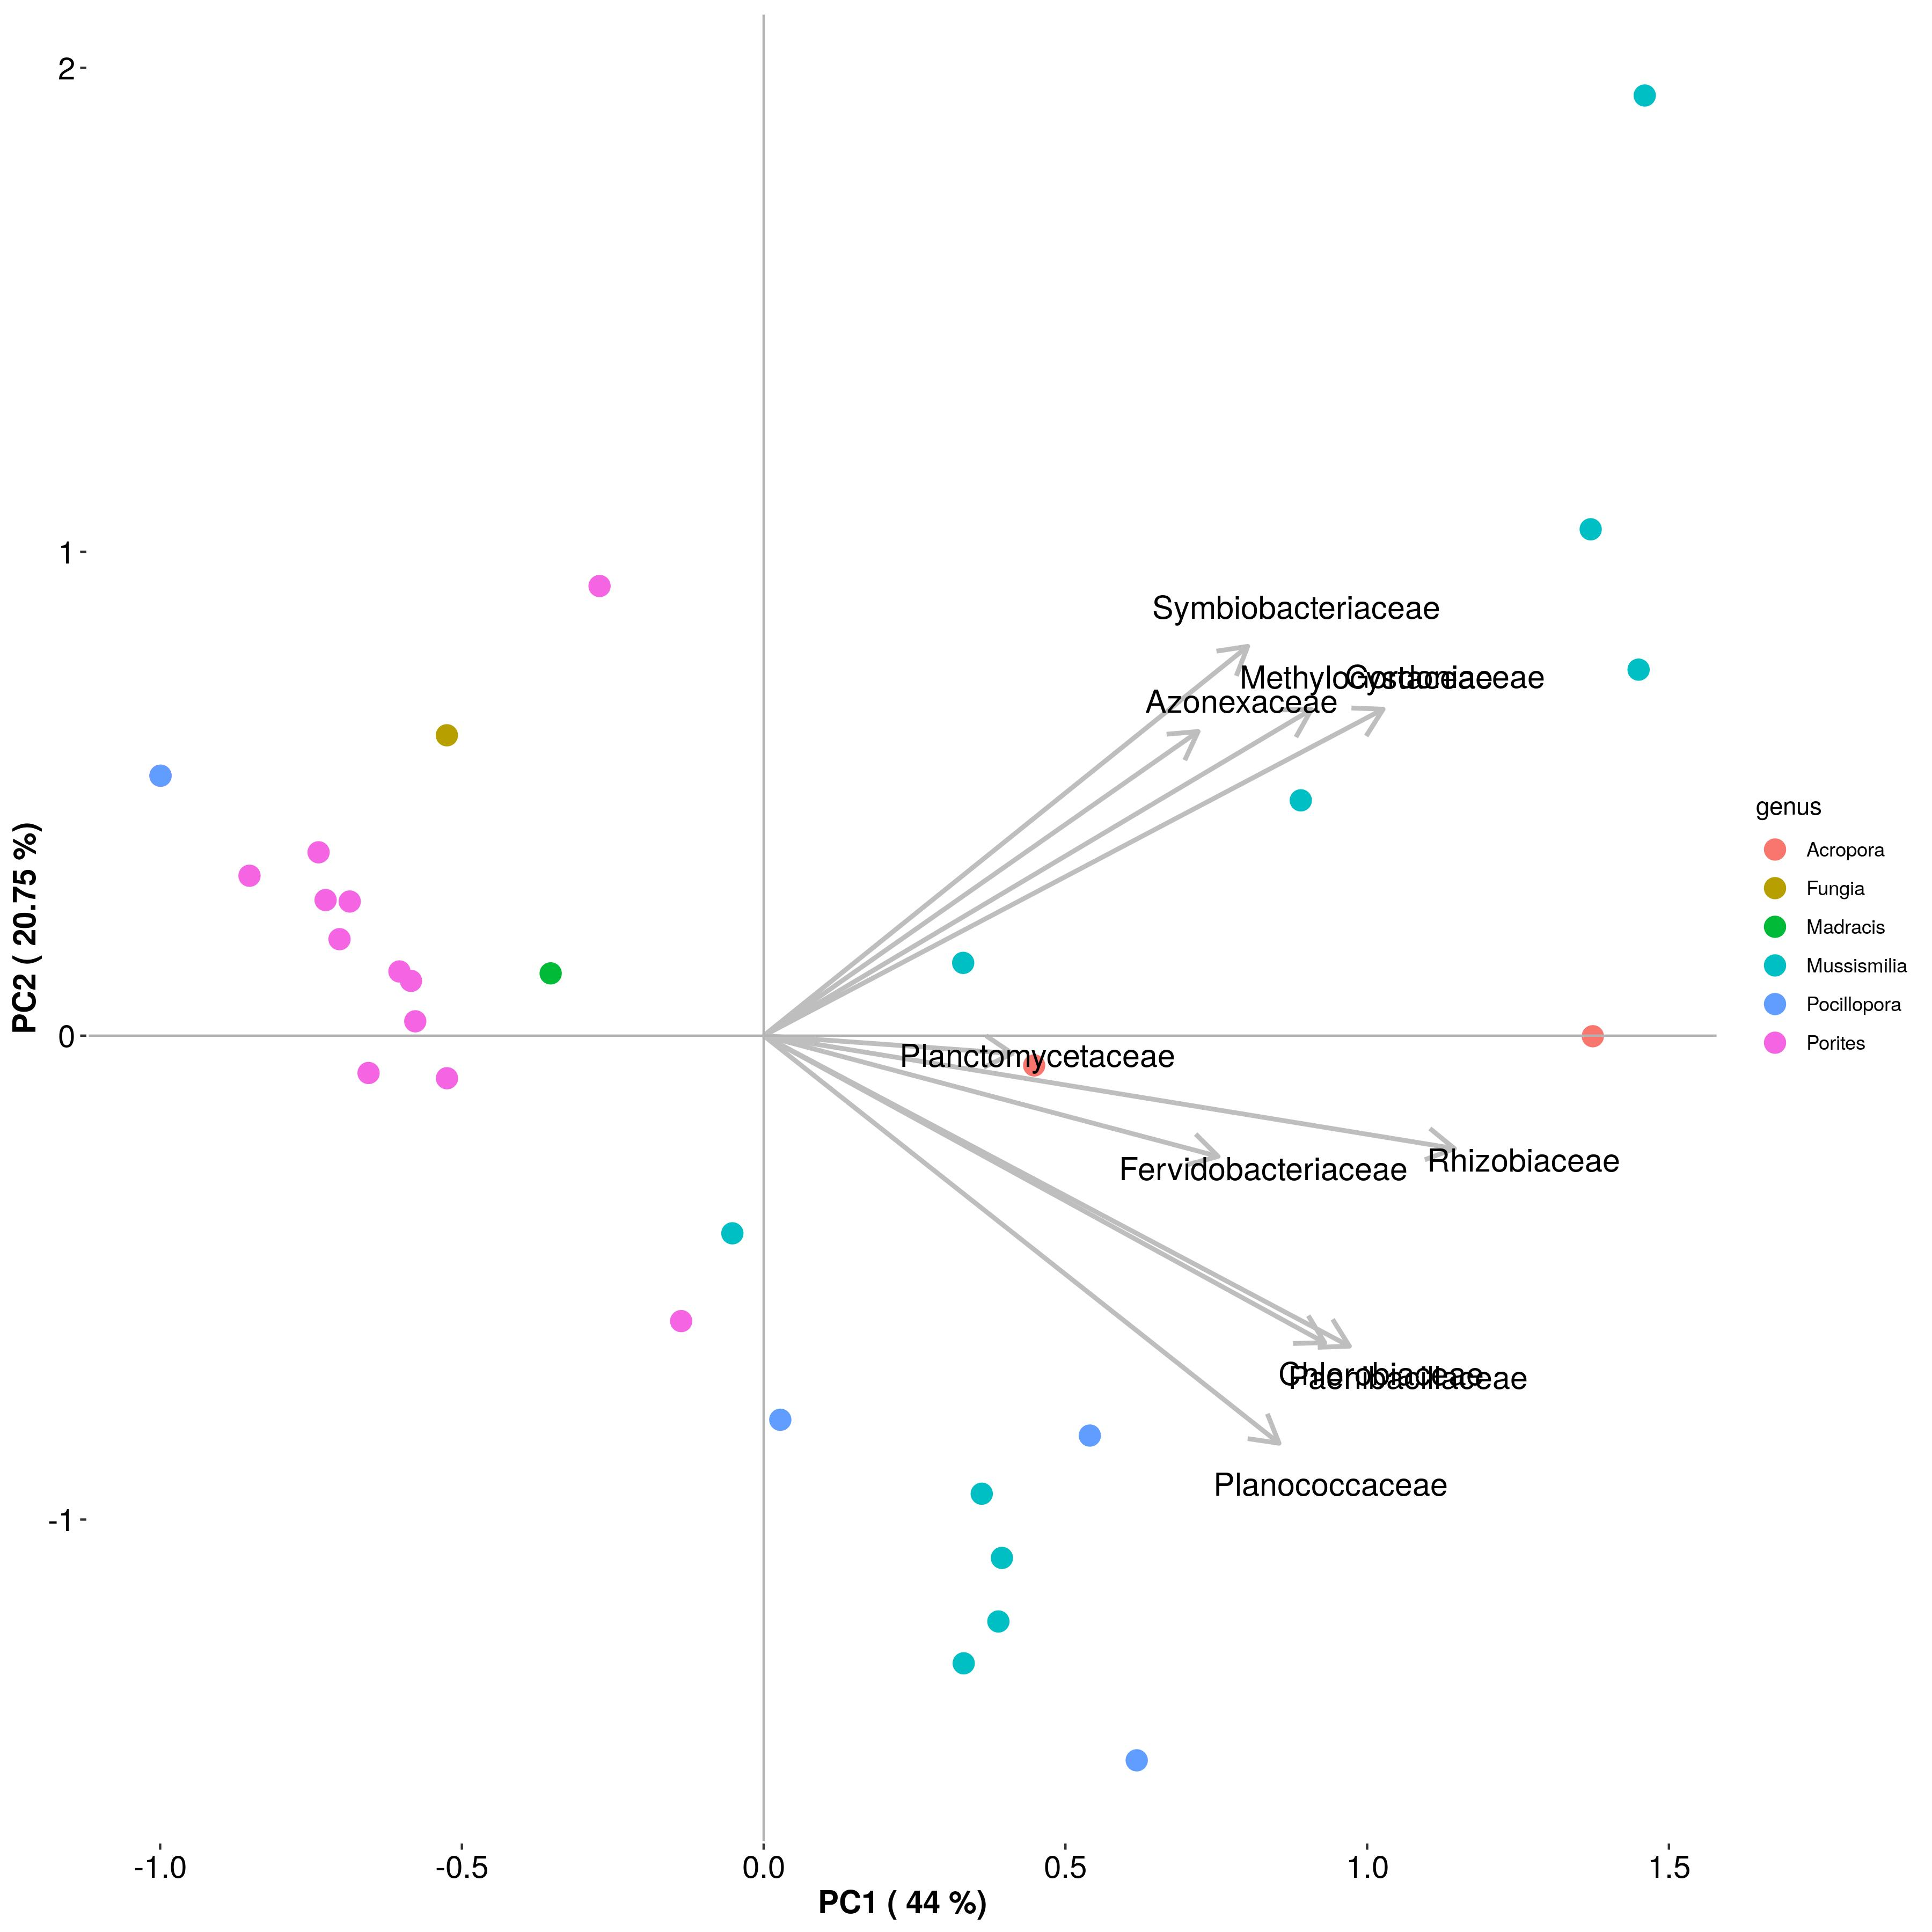
\includegraphics[scale=0.3]{figures/familia/pca_corais_mg_rast_rf_supervisionado_genus_10_familias_30_10_2018.jpg}
\caption{PCA FEITO COM OS 10 FAMILIAS INDICADOS PELO RANDOM FOREST SUPERVISIONADO POR GENERO PARA FAMILIAS DE MICRORGANISMOS}
\label{fig:PCA10FAMILIASDERIVADODORFSUPERVISIONADOGENEROPFAMILIAS}
\end{figure}

\begin{figure}[H]
\centering
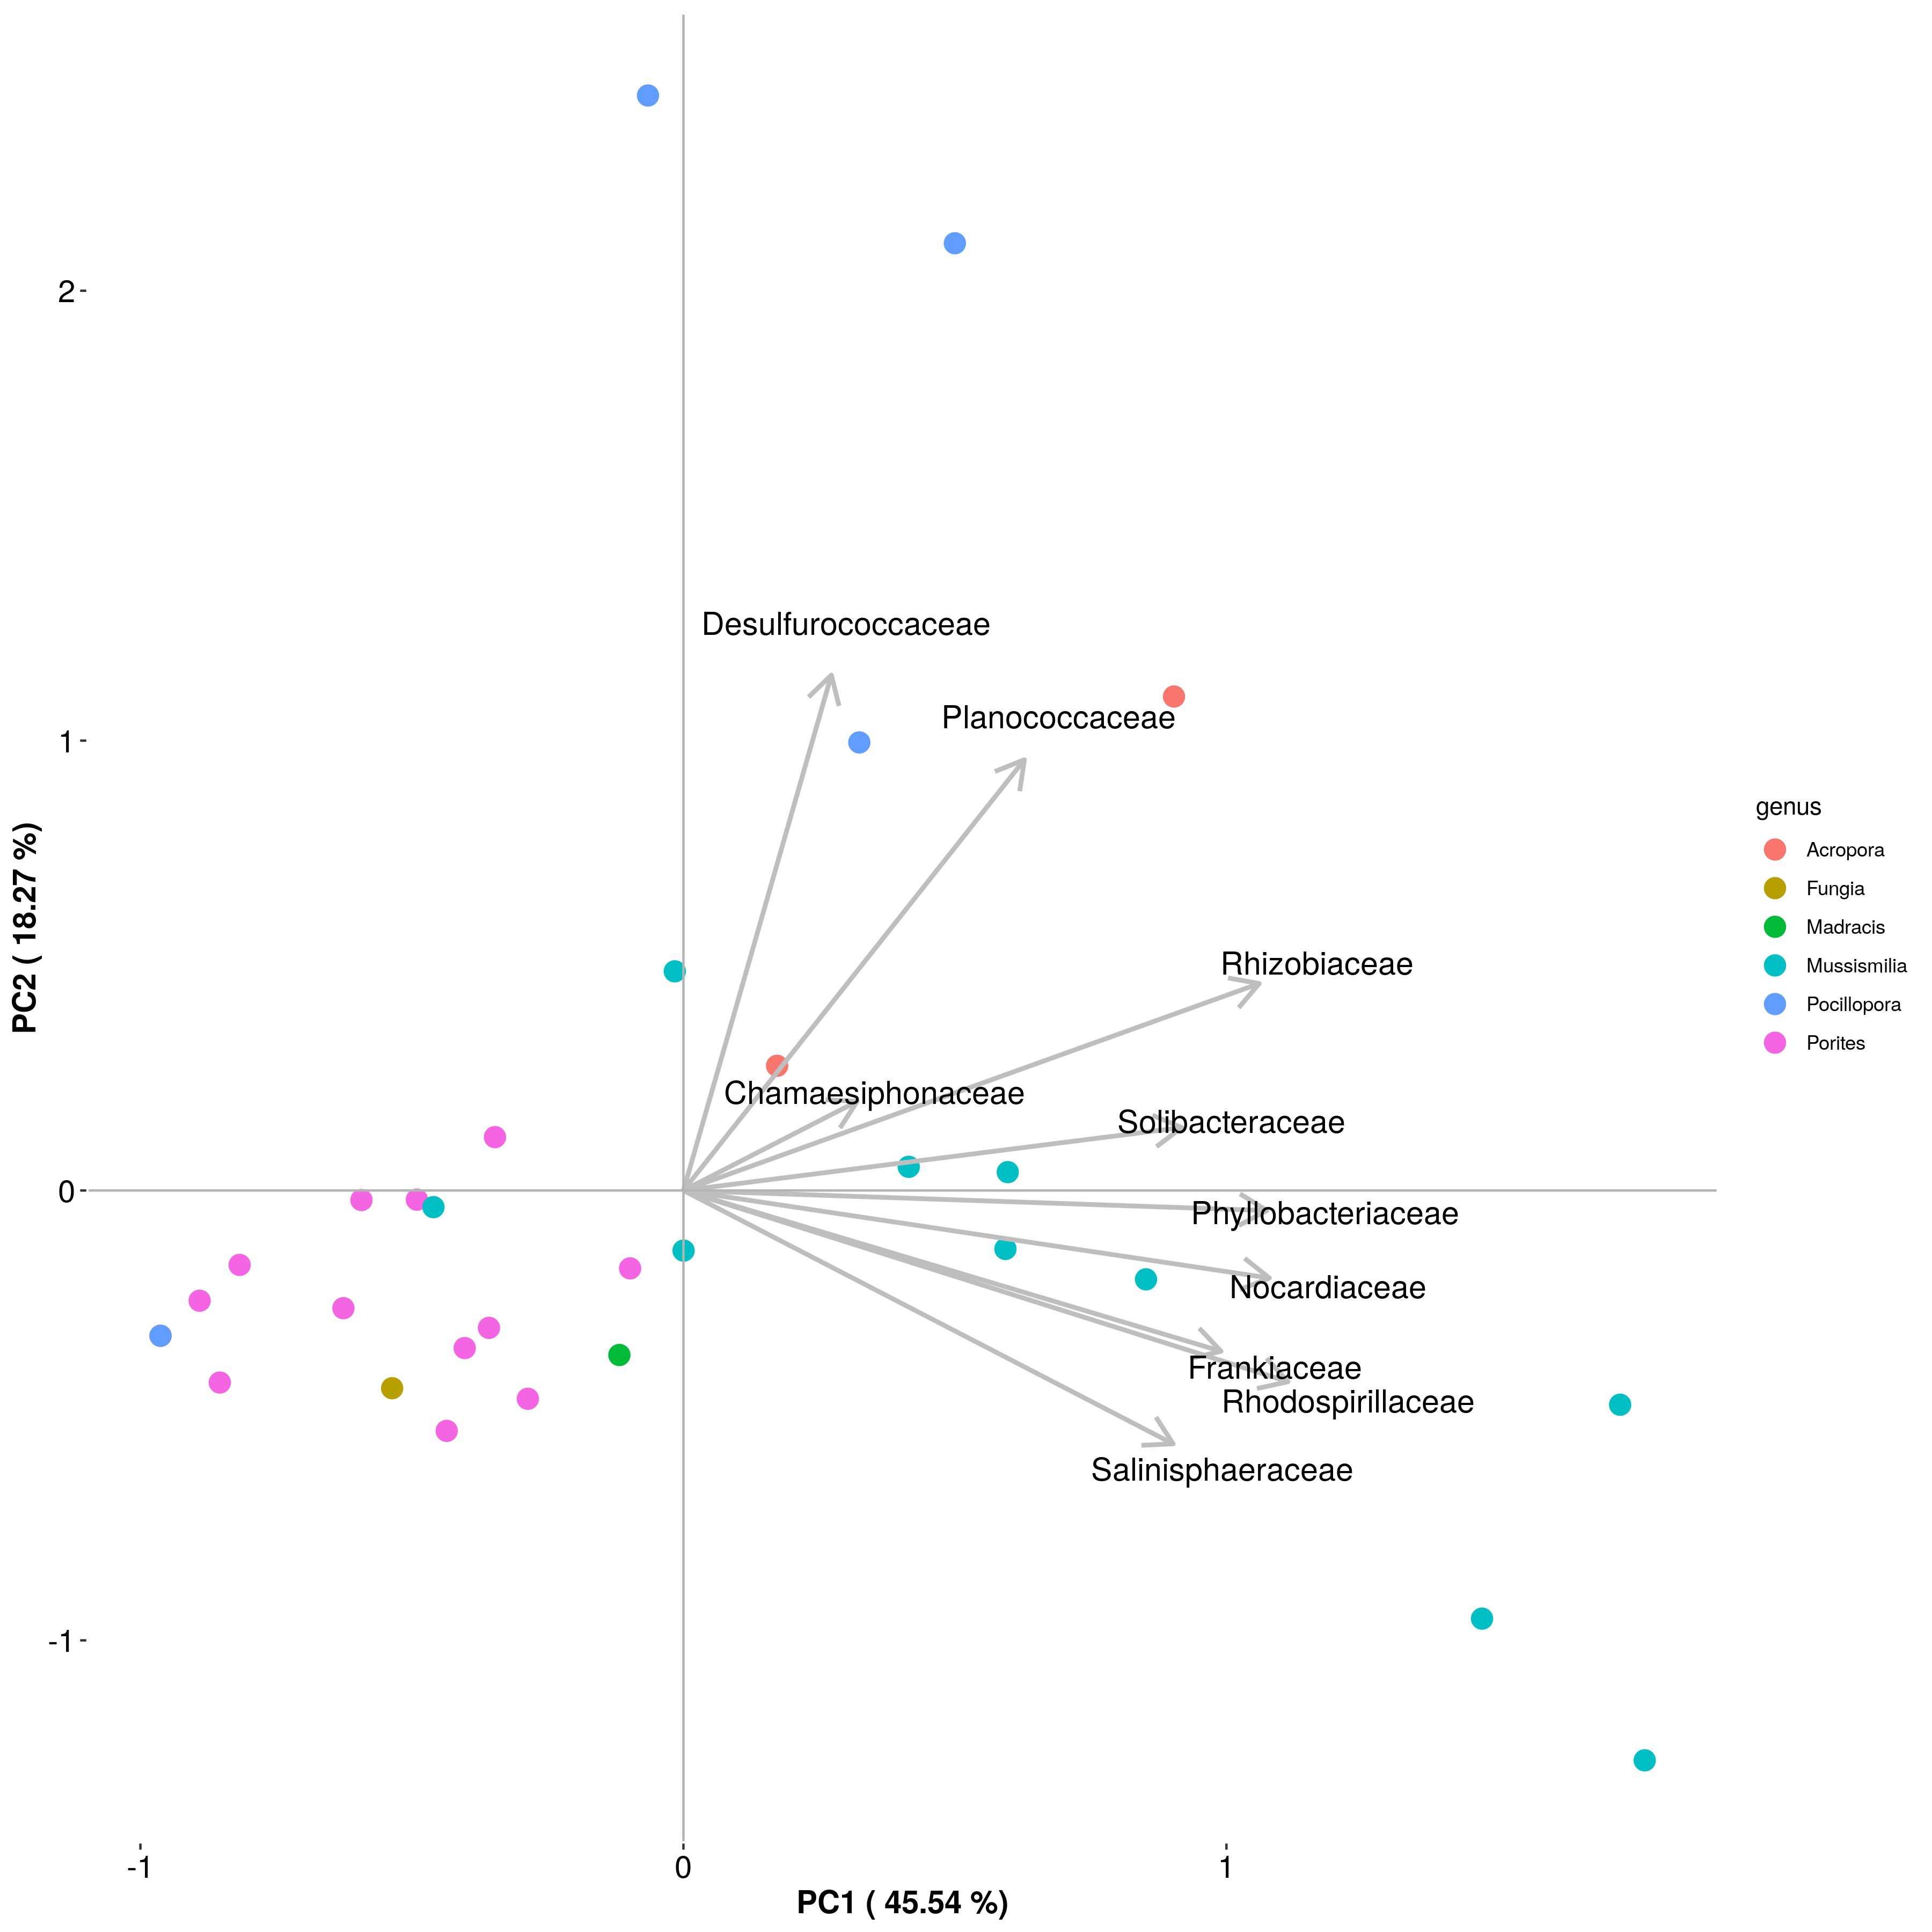
\includegraphics[scale=0.3]{figures/familia/randomforest_supervisionado_saude_corais_mgrast_familia_leticia_2018_10_30.jpeg}
\caption{RANDOM FOREST SUPERVISIONADO POR SAUDE}
\label{fig:RANDOMFORESTSUPERVISIONADOPORSAUDE}
\end{figure}

\subsection{Ferramenta microbiome no R}
O professor recomendou utilizar a seguinte ferramenta: \url{https://microbiome.github.io/microbiome/#getting-started}. Talvez seja interessante para gerar as figuras de análises.

Lendo sobre o pacote, percebi que vou precisar que os dados estejam em um formato legível pelo pacote, o formato "phyloseq". Para transformar o dado, segue a página que explica como fazer isso \url{https://joey711.github.io/phyloseq/import-data.html}.
A página recomenda baixar, entre os vários pacotes, o library(BiocManager), 

\newpage
\chapter{Functional annotation of metagenomes}
\begin{figure}
  \centering 
  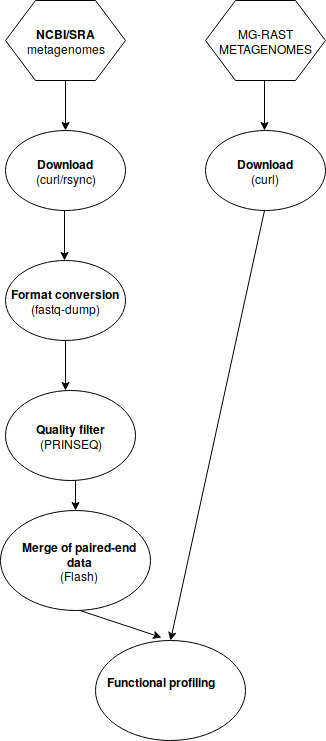
\includegraphics[width=0.7\textwidth]{figures/pipeline_functional.jpg}
  \caption{Pipeline of functional annotation}
  \end{figure}


\chapter{references}
Articles list:
\begin{itemize}
\item 10.1371/journal.pone.0071301: Relata resultados que eu acreditava ter sido a primeira a encontrar
\item 10.1038/nature14486: reconstruction of microorganism's genomes we use
\item 10.1038/nmicrobiol.2016.48: three of life, including the Candidate Phyla Radiation
\item 10.1146/annurev.micro.57.030502.090759: speaks about the uncultured majority of microorganisms
\item  10.1038/ismej.2016.174: revision of rare biosphere
\item 10.1038/nrmicro3400: another revision of rare biosphere
\item 10.1126/science.1224041: metabolic activities of Candidatus Parcubacteria, one of super-phyla of CPR
\item 10.1128/MMBR.00009-08: Revision of bioinformatic methods and steps for metagenomic
\item 10.1186/s40168-018-0428-1: Sponge as holobiont. Note: This article has a important information about microbial ecology: 
"Network and modeling analyses aim to disentangle the strength and nature (positive, negative, or neutral) of the interactions and predict their dynamics. Bacteria-bacteria network analysis of the core microbiota in different sponge species has revealed a low connective network with very few strong and many weak unidirectional interactions (i.e., amensalism [−/0] and commensalism [+/0] prevailed over cooperation [+/+] and competition [−/−]. These findings are consistent with mathematical models that predict that weak and non-cooperative interactions help to stabilize highly diverse microbial communities, whereas cooperation yields instability in the long term by fueling positive feedbacks"
\item 10.1016/j.tim.2009.09.004: Microbial disease and the coral holobiont
\item 10.3389/fmicb.2017.00618: Comparative Metagenomics of the Polymicrobial Black Band Disease of Corals
\item 10.1038/nrmicro1643: The role of ecological theory in microbial ecology
\item 10.1038/nrmicro3218: Explaining microbial genomic diversity in light of evolutionary ecology
\item 10.1111/j.1462-2920.2009.01935.x: Metagenomic analysis of stressed coral holobionts
\item 10.1038/nature06810: Functional metagenomic profiling of nine biomes
\item 10.3389/fcimb.2014.00176: Microbes in the coral holobiont: partners through evolution, development, and ecological interactions
\item 10.1038/ismej.2015.39: The coral core microbiome identifies rare bacterial
taxa as ubiquitous endosymbionts
\item 10.1111/j.1462-2920.2007.01383.x: Metagenomic analysis of the microbial community
associated with the coral Porites astreoides
\item  10.1038/nmicrobiol.2015.32: Metagenomics uncovers gaps in amplicon-based
detection of microbial diversity
\item 10.1038/ismej.2016.45: Challenges in microbial ecology: building predictive
understanding of community function and dynamics
\item 10.1111/j.1462-2920.2009.02113.x: Microbial functional structure of Montastraea faveolata,
an important Caribbean reef-building coral, differs
between healthy and yellow-band diseased colonies
\item 10.1111/j.1758-2229.2010.00234.x: 
\item 10.1038/ismej.2011.116: Assessing the complex sponge microbiota: core, variable and species-specific bacterial communities
in marine sponges
\end{itemize}

\chapter{Softwares, instalacao e linhas}

Instalar o kraken-biome

\begin{tcolorbox}[width=6.0in]
	- Folder: \textit{/home/leticia}\\
	- Command: \textit{pip install kraken-biom}\\
	- Site: \textit{https://github.com/smdabdoub/kraken-biom}
\end{tcolorbox}

Para atualizacao: \\
git commit \\
git push origin master \\

Para transferencia: \\
maquina remota para local:
scp leticia.cavalcante@login.sdumont.lncc.br:/scratch/ebiodiv/leticia.cavalcante/ncbi/ncbi.txt /home/leticia/Documentos/dados

\section{Profilling metagenomes}

\chapter{Fundamentos teoricos}


\chapter{Meetings}

\chapter{Escrita do artigo}

\subsection{30 de outubro 2018}
Na reuniao com Amaro, Miguel e o professor, mostrei os slides contendo os resultados obtidos com analises dos metagenomas utilizando a base de dados definitiva. Foram levantadas as seguintes questoes:
\begin{itemize}
\item As analises por familias não nos disseram muita coisa, alem de nao conter familias dos grupos nao cultivados por nao existir tal resolucao taxonomica. Por isso, utilizaremos apenas filo para trabalhar
\item Fazer um PCA utilizando especies de coral sem identificar status de saude visualmente
\item Fazer um PCA utilizando apenas amostras de corais saudaveis, identificando apenas genero
\end{itemize}
Tipo, se quero ver a diferenca existente entre as comunidades de generos de corais diferentes, devo fazer a analise só utilizando saudaveis em um caso e em outro sem identificar o estado de saude.

\begin{itemize}
\item Fazer um pca identificando apenas corais saudaveis e doentes, sem identificar visualmente o genero 
\item Fazer um pca utilizando apenas corais doentes
\item utilizar mais filos indicados pelo random forest para fazer o pca
\item PCA por especie
\item Procurar por amostras de madracis que o professor trabalho - FEITO
\item fazer uma planilha simplificada para Miguel e Amanda - FEITO (re-enviar a planilha, visto que encontrei as amostras e as incluirei na planilha de metagenomas)
\end{itemize}

\section{30 de novembro}
Visto que as figuras não ficarão prontas até o dia da reunião 02/12, eu conversei ontem com o professor sobre o que falar nessa reunião e ele pediu para que aprensentássemos a estrutura proposta do artigo em vez de remarcar. Eu já tinha uma estrutura de tópicos do artigo pronta, arquivo: topic\_paper.odt na pasta papers. Mostrei a Amanda, para saber se estava claro. Ela me ajudou a re-estrutura a parte dos results, com quais perguntas quero responder com as figuras que produzirei. Ficou da seguinte maneira:\\

\begin{enumerate}
\item Pergunta: Quais os filos mais abundantes e qual fator faz com que a abundância desses variem? 
	\begin{itemize}
	\item Fator saude: Existe diferença na abundância desses mais abundantes entre corais com diferentes estados de saúde?\\
	\textbf{Barplot, com X sendo corais saudáveis e doentes}
	\item Fator localidade: Existe diferença na abundância desses mais abundantes entre corais com diferentes localidades?\\
	\textbf{Boxplot, com X sendo diferentes localidades}
	\item Fator desenvolvimento: Existe diferença na abundancia desses mais abundantes entre corais com diferentes tipos de desenvolvimento?\\
	\textbf{Barplot, com X sendo diferentes tipos de desenvolvimento}
	\end{itemize}
\item Pergunta: A estrutura da comunidade difere quanto a:
	\begin{itemize}
	\item Estado de Saude?
		\begin{itemize}
		\item nMDS de healthy vs diseased
		\end{itemize}
	\item Localidade? 
		\begin{itemize}
		\item nMDS de diferentes localidades
		\end{itemize}
	\item Desenvolvimento?
	\end{itemize}
\item Pergunta: Qual a biosfera rara? Quais filos são ubíques?
Tabela suplementar sugerida pela Amanda, em que as linhas são filos e as colunas será raridade a 1\% e raridade a 5\% e ubiquidade em 50\% das amostras e 75\%? 
Maneiras de visualizar?
\end{enumerate}

 \bibliographystyle{apalike}
 \bibliography{ref}



 \end{document}
